% =============================================================================
% thesis.tex — Root document
%
% Master Thesis: "Zero-Shot Nutrient and Quantity Association using
%                 OCR-Guided Semantic Graph Matching"
% Author:        Moustafa Hamada
% Programme:     M.Sc. AI & Data Science (THD + USB)
%
% Build recipe:  xelatex × 3 + bibtex   (recommended — matches the chapter
%                workflow; the engine is detected automatically below)
%   or:          latexmk -xelatex thesis.tex
%   or:          latexmk -pdf     thesis.tex   (pdfLaTeX; also supported)
%
% Structure:
%   thesis.tex       (this file — root, preamble, document structure)
%   title.tex        (THD template — title page; consumes the variables below)
%   declaration.tex  (THD template — declaration of originality)
%   main.tex         (\input{}s the individual chapter files)
%   Chapter_2_Background.tex
%   Chapter_3_Related_Work.tex
%   references.bib   (105-entry cleaned bibliography)
% =============================================================================

\documentclass[a4paper,11pt,twoside,openright,parskip=half]{scrbook}
% ----------------------------------------------------------------------
% Engine detection
%   Lets the same source compile under XeLaTeX/LuaLaTeX (UTF-8 native,
%   Unicode fonts) and under pdfLaTeX (8-bit; needs inputenc + fontenc).
% ----------------------------------------------------------------------
\usepackage{iftex}

% ----------------------------------------------------------------------
% Encoding (pdfLaTeX only — XeLaTeX/LuaLaTeX read UTF-8 natively)
% ----------------------------------------------------------------------
\ifPDFTeX
  \usepackage[utf8]{inputenc}
  \usepackage[T1]{fontenc}
\fi

% ----------------------------------------------------------------------
% Language
% ----------------------------------------------------------------------
\usepackage[english]{babel}

% ----------------------------------------------------------------------
% Mathematics — required for Chapter 2's equation* and \text{} usage
% ----------------------------------------------------------------------
\usepackage{amsmath, amssymb}

% ----------------------------------------------------------------------
% Graphics, tables, formatting
% ----------------------------------------------------------------------
\usepackage{graphicx}
\usepackage{booktabs}
\usepackage{relsize}
\usepackage{ifthen}
\usepackage{rotating}
% ----------------------------------------------------------------------
% URLs and hyperlinking
% ----------------------------------------------------------------------
\usepackage{url}
\usepackage[
    colorlinks=false,
    pdfborder={0 0 0},
    bookmarksopen=true,
    bookmarksnumbered=true
]{hyperref}

% ----------------------------------------------------------------------
% Typography — Linux Libertine (THD template default)
%   The libertine package is engine-aware: under XeLaTeX/LuaLaTeX it loads
%   fontspec and uses the OpenType Libertine fonts; under pdfLaTeX it uses
%   the T1 Type1 fonts. No change needed either way.
% ----------------------------------------------------------------------
\usepackage{libertine}
\usepackage{microtype}   % micro-justification; clears routine prose overfulls
% ----------------------------------------------------------------------
% Page layout — headers and footers
% NOTE: If your professor's template uses different header/footer styling,
%       replace this whole block with theirs.
% ----------------------------------------------------------------------
\usepackage{fancyhdr}
\pagestyle{fancy}
\fancyhf{}
\fancyhead[LE,RO]{\thepage}
\fancyhead[RE]{\nouppercase{\leftmark}}
\fancyhead[LO]{\nouppercase{\rightmark}}
\renewcommand{\headrulewidth}{0.4pt}
\fancypagestyle{plain}{%
  \fancyhf{}%
  \fancyfoot[C]{\thepage}%
  \renewcommand{\headrulewidth}{0pt}%
}

% ----------------------------------------------------------------------
% Float placement control
%   1. placeins provides \FloatBarrier.
%   2. A FloatBarrier before every \section keeps a float inside the
%      section that introduces it (stops cross-section drift). This is an
%      explicit redefinition rather than placeins' [section] option,
%      because that option hooks \@startsection — which KOMA-Script's
%      sectioning commands do not use, so [section] can silently do nothing
%      under scrbook. The redefinition below is class-independent and
%      handles the *, [short], and {long} forms of \section unchanged.
%   3. The float fractions let a figure/table fill more of a page before
%      LaTeX banishes it to a float-only page.
% ----------------------------------------------------------------------
\usepackage{placeins}
\renewcommand{\topfraction}{0.9}
\renewcommand{\bottomfraction}{0.8}
\renewcommand{\textfraction}{0.07}
\renewcommand{\floatpagefraction}{0.75}
\setcounter{topnumber}{3}
\setcounter{bottomnumber}{2}
\setcounter{totalnumber}{5}
\raggedbottom

% ----------------------------------------------------------------------
% Line breaking — last-resort stretch to avoid overfull \hbox
% ----------------------------------------------------------------------
\setlength{\emergencystretch}{3em}
\tolerance=1000     % accept slightly loosebr lines instead of overflowing; raise toward 2000 if needed
% =============================================================================
% Title-page variables — consumed by title.tex (THD template)
% =============================================================================
% These commands are referenced inside title.tex. Update the TODO entries
% with your real information before final submission.
% =============================================================================

\newcommand{\faculty}{Angewandte Informatik}
\newcommand{\studies}{Artificial Intelligence and Data Science}
\newcommand{\degree}{Master of Science (M.Sc.)}

% TODO: replace with your real German thesis title
\newcommand{\thesistitleDE}{Zero-Shot-Assoziation von N\"ahrstoffen und Mengen mittels OCR-gest\"utztem semantischem Graph-Matching}

% English title
\newcommand{\thesistitleEN}{Zero-Shot Nutrient and Quantity Association using OCR-Guided Semantic Graph Matching}

% TODO: replace with your full name as it should appear on the title page
\newcommand{\student}{Moustafa Hamada}

% Matrikelnummer (THD student ID)
\newcommand{\matrnr}{12401478}

% TODO: Stammnummer (USB student ID); leave empty {} if you don't have one
\newcommand{\stammnr}{}

% TODO: Submission date (e.g. "September 2026" or "10. September 2026")
\newcommand{\submissiondate}{September 2026}

% TODO: Primary supervisor (Pr\"ufungsleitung) — name, title, affiliation
\newcommand{\supervisor}{Prof.\ Dr.\ Andreas Fischer\\Technische Hochschule Deggendorf}

% TODO: Secondary supervisor (Erg\"anzende Pr\"ufende); leave empty {} if none
\newcommand{\secsupervisor}{}

% ----------------------------------------------------------------------
% PDF metadata
% ----------------------------------------------------------------------
\hypersetup{
  pdftitle  = {\thesistitleEN},
  pdfauthor = {\student},
  pdfsubject = {M.Sc. Thesis, AI \& Data Science, THD + USB}
}

% =============================================================================
\begin{document}
% =============================================================================

% ----------------------------------------------------------------------
% Title page and declaration (provided by THD template; do not edit here)
% ----------------------------------------------------------------------
\setkomafont{title}{\huge \scshape}
\begin{titlepage}
\begin{center}
	{\usekomafont{subject}
	Technische Hochschule Deggendorf\\
	Fakultät \faculty\par}
	\vspace{.2cm}
{\Large Studiengang \studies\\}
\vspace{6\baselineskip}
{\Huge\usekomafont{title}\thesistitleDE\par}
\vspace{1cm}
{\Huge\usekomafont{title}\thesistitleEN\par}
\vspace{6\baselineskip}

\usekomafont{publishers}
Masterarbeit zur Erlangung des akademischen Grades:

	\vspace{.2cm}
	\emph{\degree}
	\vspace{.2cm}

an der Technischen Hochschule Deggendorf\\
\end{center}
\vfill
\parbox[t]{.4\textwidth}{\usekomafont{author}
	Vorgelegt von:\\
	\student\\
	Matrikelnummer:  \matrnr\par
	\ifthenelse{\equal{\stammnr}{}}{}{
	Stammnummer: \stammnr\par
	}
	\vspace{\baselineskip}
	Am: \submissiondate\par
}
\hfill
\parbox[t]{.4\textwidth}{\usekomafont{author}
Prüfungsleitung:\\
\supervisor%

\ifthenelse{\equal{\secsupervisor}{}}{}
{%
\vspace{\baselineskip}
Ergänzende Prüfende:\\
\secsupervisor%
}}
\end{titlepage}
\cleardoublepage\par

\input{declaration}

% ----------------------------------------------------------------------
% Front matter: Roman numerals, no chapter numbering
% ----------------------------------------------------------------------
\frontmatter

% \input{abstract}          % NOTE: uncomment when abstract.tex exists
% \input{acknowledgements}  % NOTE: uncomment when acknowledgements.tex exists

\tableofcontents
% \listoffigures            % NOTE: Chapter 4 now has several figures — uncomment if wanted
% \listoftables             % NOTE: Chapter 4 now has a table — uncomment if wanted

% ----------------------------------------------------------------------
% Main matter: Arabic numerals, chapter numbering on
% ----------------------------------------------------------------------
\mainmatter
% !TEX root = thesis.tex
% =============================================================================
% main.tex
%
% Chapter dispatcher for the thesis.
% \input{} into thesis.tex from inside \mainmatter, so chapters are numbered
% in Arabic and the bibliography is appended after.
%
% Add new chapters here as they are written. Order matters — chapters are
% numbered by their \input{} order.
% =============================================================================

% ----------------------------------------------------------------------
% Chapter 1 — Introduction
% ----------------------------------------------------------------------
% !TEX root = thesis.tex
% =====================================================================
%  CHAPTER 1 — INTRODUCTION
%  Zero-Shot Nutrient and Quantity Association using
%  OCR-Guided Semantic Graph Matching
%  Moustafa Hamada | THD + USB
%
%  Build: scrbook, XeLaTeX + BibTeX. Citations: \cite{}.
%  Cross-refs: Chapter~\ref{} / Section~\ref{}  (matches the Ch2/Ch5/Ch6 body).
%
%  REVISION NOTES (this pass):
%    - Motivation no longer lists specific downstream applications; the value of
%      structured label data is stated generally.
%    - Motivation now names the large-VLM shortcut and its two costs (price and
%      the black-box lack of transparency), and this tension is carried through
%      the problem statement, the gap, and the research questions.
%    - A teaser figure reuses the Ch2 association-task image (Option A: same
%      asset, NEW label, teaser caption pointing to Ch2 — no other file touched).
%    - Aim section adds a central research question and a paragraph mapping the
%      five sub-questions to the dimensions of the research gap.
%
%  FORWARD REFERENCES (labels defined in the other chapter files):
%    chap:background   (Ch2)
%    ch:related-work   (Ch3 — note: this chapter keeps the ch: prefix, not chap:)
%    chap:methodology  (Ch4)
%    chap:evaluation   (Ch5)
%    chap:experiments  (Ch6)
%    chap:conclusion   (Ch7 — NOT YET WRITTEN. Use exactly this label in the
%                       conclusion file so the \ref here resolves; until then
%                       LaTeX prints "??" for that one reference only.)
%
%  FIGURE ASSET (reused from Ch2, guarded by \IfFileExists so it compiles before
%  the file is present):
%    association_task.png   ->  \label{fig:intro-association-task}
%
%  CITED KEYS — all already appear in references.bib (reused from Ch3/Ch4):
%    nagayi2025foodocr, arief2026halalbench, yu2020pick, hwang2021spade
%
%  NOTE: \mcode{} is defined *inside* Chapter 4, so it is NOT available here.
%  Any code-like literal in this chapter uses \texttt{} instead.
%
%  LABELS IN THIS FILE:
%    chap:introduction
%    sec:intro-motivation, sec:intro-problem, sec:intro-gap,
%    sec:intro-questions, sec:intro-contributions, sec:intro-outline
% =====================================================================

\chapter{Introduction}\label{chap:introduction}

Packaged food and dietary supplements carry a nutrition label, and for most
products that printed panel is the main public record of what the product
contains. Having its contents as structured data --- one clean record per
nutrient value --- is far more useful than the image itself, because structured
records can be searched, compared, and processed automatically, while an image
cannot. This thesis builds a system that reads the label image, works out which
number belongs to which nutrient, and returns the result as a set of such
records, without being trained on the labels it must read.

\section{Motivation}\label{sec:intro-motivation}

A nutrition or supplement label is a small, dense document. It lists the
product's nutrients, the amount of each, the unit that amount is measured in, and
the reference basis the amount is stated under, such as per 100 grams or per
serving. Written as a record, one such line becomes the four-field tuple
$\langle\text{nutrient},\,\text{quantity},\,\text{unit},\,\text{context}\rangle$.
A person can read a panel one line at a time, but many uses need the data for many
products at once, in a form a program can process, and producing that by hand
does not scale: the set of products is open and grows constantly, with tens of
thousands of new layouts appearing each year, each of which would have to be
transcribed and checked. An automatic method that reads the label image and
returns the records directly is therefore worth having.

One modern shortcut is to hand the whole task to a large vision--language model:
give it the label image and ask it to return the records in a single step. Such a
model needs no task-specific training and copes with many layouts, which makes it
an obvious first choice. It comes with two costs, though, that matter for this
setting. The first is price: calling a large model on every label is expensive,
and the expense grows with the number of labels. The second, and the more serious
here, is that the model is a black box. It returns the records in one opaque step,
with no intermediate that can be inspected, so when a value comes out wrong there
is no way to tell whether the mistake was in the reading, the classification, or
the linking, and no record tying an output back to the evidence that produced it.
For data meant to be processed automatically, being unable to check or trace a
result is a real limitation. What is wanted, then, is a method that is automatic
like the model, but also cheap to run and open to inspection at every step. That
is the method this thesis sets out to build.

\section{Problem Statement}\label{sec:intro-problem}

The first step, optical character recognition (OCR), reads the characters in the
image and returns them as text tokens, each with a bounding box and a confidence
score. This is necessary but not sufficient. OCR says what text is on the label
and where it sits; it does not say how the pieces belong together. A label carries
many nutrient names and many numbers, and the real work is to join each number to
the nutrient it describes, then attach the right unit and the right context. This
joining step is the association problem, and it is the heart of the task. Seeing
the tokens \texttt{Magnesium}, \texttt{400}, and \texttt{mg} on a label is not the
same as knowing that the three form one record; a label may hold twenty nutrients
and forty numbers, and a single wrong link already produces a wrong record.
Figure~\ref{fig:intro-association-task} shows the task end to end: the label
enters on the left, its classified tokens sit in the middle, and the finished
records leave on the right, with the association step marked by the question mark.

\begin{figure}[htbp]
  \centering
  \IfFileExists{association_task.png}{%
    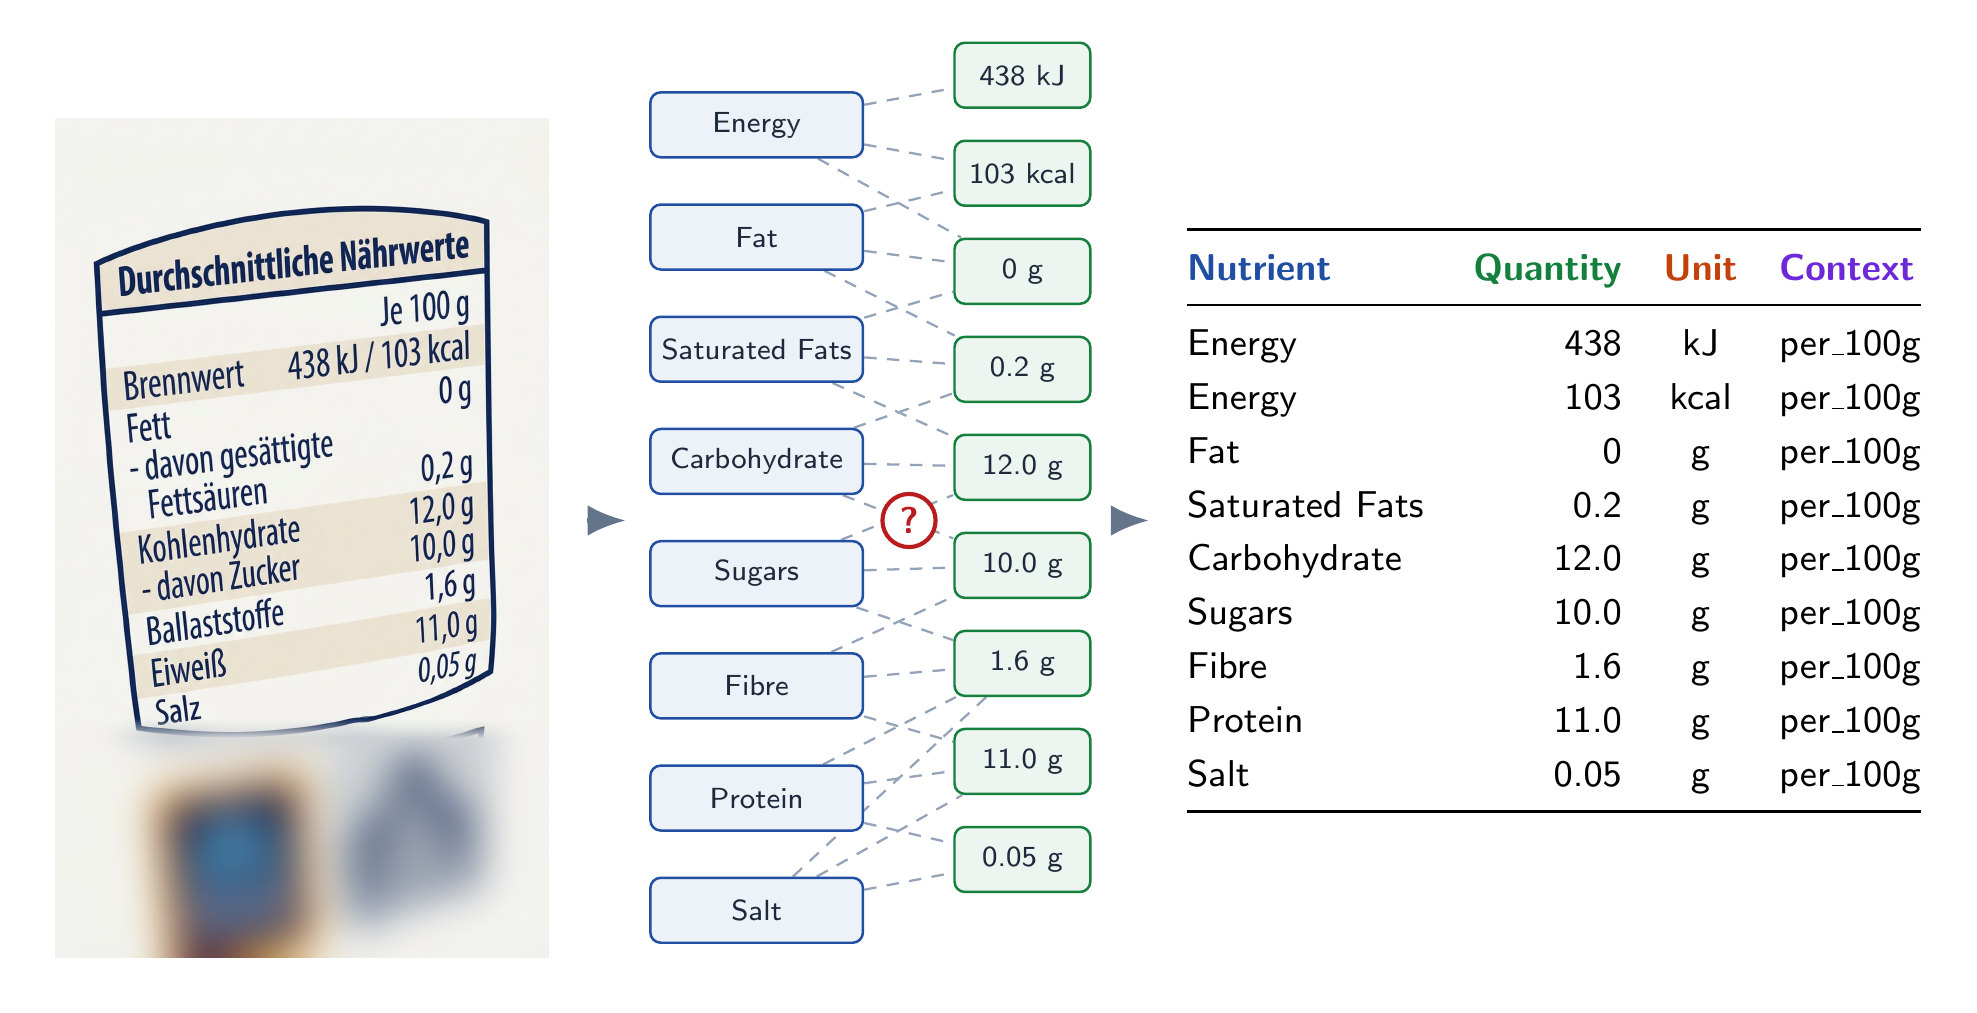
\includegraphics[width=\textwidth]{association_task.png}%
  }{%
    \fbox{\parbox[c][0.30\textheight][c]{0.9\textwidth}{\centering\itshape
      Figure file \texttt{association\_task.png} not found --- save the
      association-task figure to this path.}}%
  }
  \caption[The extraction task at a glance]{The extraction task at a glance, on
    one nutrition label. \emph{Left:} the input image. \emph{Middle:} the same
    tokens after classification, with nutrient names on one side and quantities
    on the other. \emph{Right:} the target records, one four-field tuple per row.
    The association step, marked by the question mark, must tie each quantity to
    the correct nutrient; because a label holds many of each, one wrong link
    already yields a wrong record. The same figure, with the full definition,
    appears in Chapter~\ref{chap:background}.}
  \label{fig:intro-association-task}
\end{figure}

Several properties of real labels make association hard. The labels are
multilingual: a single panel often mixes German and English, and others across
the corpus add French, Dutch, Italian, and Spanish. They are laid out as dense
tables, sometimes photographed at an angle or printed on curved packaging, so the
geometry is not clean; both failure modes are well documented for food-packaging
OCR~\cite{nagayi2025foodocr}. Most of all, the labels are multi-context. The same
nutrient is frequently reported more than once --- once per 100 grams and once
per serving, for example --- so one nutrient name lines up with several numbers,
and the only thing that separates those numbers is the column each sits in.
Across the corpus used here, about two-thirds of nutrient instances carry more
than one value in this way. A method that reads the label line by line cannot tell
these values apart; it has to reason about the column layout, which is what makes
a simple left-to-right or top-to-bottom reading insufficient.

The task also has to be solved without training on the labels themselves. There
is no annotated corpus of supplement labels with record-level ground truth to
learn from, and building one for a fixed set of products would not help for long,
since the set of products is open and keeps growing. The wide spread of real
labels makes this concrete --- a large multilingual benchmark finds that even
strong engines fail on scripts they were not built for~\cite{arief2026halalbench}
--- so any method that depends on per-layout or per-language training cannot
scale. The system must therefore work zero-shot, on nutrient names, layouts, and
languages it has not met before, and lean on general-purpose components and
explicit rules rather than on a model fitted to the target labels. In this thesis
the constraint is taken strictly: no stage is trained or fine-tuned on the label
images, and the annotations are used only to score the output, never to build it.

The interpretability that the motivation calls for is the last requirement, and
the multi-stage design is what delivers it. Where an end-to-end model binds every
field in one opaque step, a pipeline that keeps its stages explicit --- each token
carrying its text, role, and position, and each link traceable to the rule that
made it --- can be inspected when a record is wrong and corrected at the stage
that caused it. This thesis therefore treats interpretability as a design goal on
equal footing with accuracy, and its components are chosen so that the reasoning
behind each record stays visible.

\section{Limitations of Existing Approaches}\label{sec:intro-gap}

Existing methods each solve part of this problem but give up something the task
needs. Chapter~\ref{ch:related-work} reviews them in full; only the shape of the
gap is given here. Pipelines built on OCR followed by regular expressions or
hand-written rules are transparent and need no training, but they break on the
structural problems above --- dense rows of numbers, several value columns, mixed
languages, and broken layouts. Graph-based extractors such as PICK~\cite{yu2020pick}
and SPADE~\cite{hwang2021spade} rightly treat extraction as a relational problem
and reason over the two-dimensional layout, but they learn their structure end to
end from annotated corpora, so they are not built for zero-shot use across unseen
multilingual labels, and no such annotated corpus of supplement labels exists to
train them on. End-to-end vision--language models, already discussed above, remove
the need for training data but return their records from a single step that is
costly to run and cannot be inspected, with no audit trail from an output back to
its evidence.

Read together, these approaches leave one corner of the design space empty. None
is at once zero-shot, interpretable, relational, and able to handle multilingual
labels: the regex pipelines are not robust, the graph extractors are not
zero-shot, and the end-to-end models are not interpretable. No existing method
reconstructs four-field nutrition tuples from arbitrary, multilingual, previously
unseen supplement labels without task-specific training while keeping every stage
open to inspection. That corner is what this thesis sets out to occupy.

\section{Aim and Research Questions}\label{sec:intro-questions}

The aim of this thesis is to build a modular, interpretable, zero-shot pipeline
that reconstructs the four-field tuple
$\langle\text{nutrient},\,\text{quantity},\,\text{unit},\,\text{context}\rangle$
from an arbitrary multilingual nutrition or supplement label. The approach keeps
OCR as a replaceable front-end that supplies tokens, classifies each token into a
semantic role without training on the target labels, and then solves the
association problem with an explicit graph. This graph is the central idea of the
work, named here OCR-guided semantic graph matching: the classified tokens become
nodes, and typed edges --- built by closed-form geometric and structural rules
rather than learned weights --- record which tokens are aligned in a row, share a
column, sit next to one another, or fall under the same header. The output records
are then read back out of the graph. Because the edges follow fixed rules, the
same label always gives the same edges, and every link can be traced to the rule
behind it, which keeps the association step interpretable while remaining
zero-shot.

A vision--language model is included, but deliberately confined. Rather than hand
the whole task to such a model, the pipeline uses one only at the association
step, giving it the same OCR-derived token table the graph receives and asking it
to bind the tokens into records. This variant is a point of comparison, not the
primary method, and it is set against a second use of the same class of model that
maps the raw image straight to records end to end. Comparing the graph, the
confined model, and the end-to-end model shows how much of the result comes from
structuring the problem before any field is bound, and how much comes from the
model's flexibility.

These aims come together in one central question:
\begin{quote}
Can a modular pipeline that stays zero-shot and interpretable at every stage
reconstruct the four-field tuple from arbitrary multilingual supplement labels by
matching a semantic graph over OCR tokens, and how does it compare, in both
accuracy and cost, with confining a vision--language model to the association step
and with an end-to-end vision--language model?
\end{quote}
The question restates the four properties the research gap leaves unmet ---
zero-shot, interpretable, graph-based, and multilingual --- and adds the
comparison against the black-box alternative that the motivation set up.

The pipeline is modular, so each part of this question can be tested on its own by
changing one stage while the rest is held fixed. The central question therefore
breaks into five sub-questions, each tied to one design choice and answered by
ablation in Chapter~\ref{chap:experiments}:
\begin{enumerate}
  \item Which OCR engine reads nutrition labels most accurately?
  \item Which semantic classifier detects nutrient entities most reliably?
  \item Which association engine builds better tuples, the naive geometric graph
        or the enriched, geometry-aware graph?
  \item If a vision--language model is used only at the association step, does it
        beat the graph, and how does it compare with an end-to-end
        vision--language model that maps the image directly to tuples?
  \item Which edge-creation mode builds the best row relations inside the enriched
        graph?
\end{enumerate}

Each sub-question probes one dimension of the gap. Questions~1 and~2 concern the
zero-shot reading and classification the whole pipeline stands on, so they test
whether the interpretable front-end can recover the tokens at all without
training. Questions~3 and~5 are the core of the contribution: they ask whether a
graph built from closed-form geometric rules can do the relational binding that
PICK and SPADE reach only with supervision, and whether its geometric edges are
the right mechanism for it --- the answer to those extractors' reliance on
annotated data. Question~4 makes the interpretability-and-cost trade-off
measurable, weighing the fully interpretable graph against the confined and
end-to-end uses of a black-box model --- the answer to the opacity and expense of
end-to-end extraction. Together the five cover the empty corner the gap describes,
from the reading substrate to the binding step.

\section{Contributions}\label{sec:intro-contributions}

The thesis makes the following contributions.
\begin{enumerate}
  \item A modular, fully interpretable, zero-shot extraction pipeline that
        reconstructs four-field nutrition tuples from multilingual supplement
        labels, with the intermediate output of every stage kept explicit so that
        a wrong record can be traced to the stage that caused it.

  \item Its central novelty, OCR-guided semantic graph matching: an association
        method that builds an explicit graph over semantically classified OCR
        tokens using closed-form geometric and structural edge rules, with no
        learned weights and no training on the target data. Its enriched,
        geometry-aware form keeps several value columns apart, which is where it
        earns its advantage on multi-context labels.

  \item A design that confines a vision--language model to the association
        sub-task alone, together with a controlled comparison of this confined
        model against the graph and against an end-to-end model, which isolates
        the value of structuring the problem before any field is bound and makes
        the cost of the black-box route explicit.

  \item An annotated evaluation corpus of 57 multilingual nutrition and supplement
        labels with 866 gold four-field tuples, together with a deterministic,
        fully reproducible evaluation protocol.

  \item A systematic ablation across three axes --- the OCR engine, the semantic
        classifier, and the association engine --- that separates the effect of
        each design choice on the final tuple score, and a set of empirical
        findings that follow from it: OCR is the single largest lever; the
        enriched graph's advantage over the naive one is structural and shows on
        multi-context labels; geometric row edges beat rank-based ones; confining
        a vision--language model to association beats using it end to end; and a
        clear trade-off holds between accuracy, interpretability, and runtime.
\end{enumerate}

\section{Thesis Outline}\label{sec:intro-outline}

The rest of the thesis is organised as follows.

Chapter~\ref{chap:background} fixes the vocabulary. It defines, in plain terms,
each idea the pipeline relies on --- structured extraction and association, OCR,
token normalisation, semantic role labelling, text embeddings, token enrichment,
graph representations, vision--language models, and zero-shot learning --- in the
order they appear in the pipeline.

Chapter~\ref{ch:related-work} sets these ideas against the published systems the
pipeline borrows from and departs from. It reviews OCR on food labels,
supervision-free information extraction, graph-based extraction, and zero-shot
extraction, and uses the comparison to state the research gap the thesis fills.

Chapter~\ref{chap:methodology} specifies the pipeline and the design decisions
behind it, stage by stage: OCR and token correction, semantic role
classification, token enrichment and geometry, graph construction, and
graph-based association, together with the confined vision--language association
variant. It also sets out the three ablation axes.

Chapter~\ref{chap:evaluation} describes the data and how the pipeline is scored.
It presents the 57-image corpus, the annotation schema and protocol, the four
scored fields, and the four-field and three-field tuple metrics with the matching
rules used for scoring.

Chapter~\ref{chap:experiments} presents the experiments and their results. It
answers the five questions above by ablation, changing one stage at a time across
the fourteen pipeline configurations, discusses what each comparison shows, and
analyses where the remaining errors begin.

Chapter~\ref{chap:conclusion} draws the findings together, states the limitations
of the method, and points to future work.     % NOTE: uncomment when written

% ----------------------------------------------------------------------
% Chapter 2 — Background
% ----------------------------------------------------------------------
% !TEX root = thesis.tex
% =====================================================================
%  CHAPTER 2 — BACKGROUND  (concept-only, plain-English rewrite)
%  Zero-Shot Nutrient and Quantity Association using
%  OCR-Guided Semantic Graph Matching
%  Moustafa Hamada | THD + USB
%
%  Scope: terminology only. System description (pipeline overview,
%  problem formulation) and component configs live in the methodology
%  and experimental chapters, so this chapter is a reusable concept
%  reference that later work can build on.
%
%  Build: scrbook, XeLaTeX + BibTeX. Citations: \cite{}.
%  Cross-refs: Section~\ref{} / Chapter~\ref{}  (matches the methodology body).
%  One displayed equation (cosine) uses base LaTeX only -> no new packages.
%
%  CITES (all resolve against references.bib once the 22 Background entries
%  are appended; the keys below already point at your existing entries where
%  they overlap):
%    sarawagi2008ie, pawar2017relation, long2021scene, easyocr,
%    cui2025paddleocr, manning2008ir, sproat2001normalization,
%    li2022nersurvey, palmer2010srl, zaratiana2023gliner,
%    mikolov2013word2vec, reimers2019sbert, chen2024bgem3, chow1970reject,
%    xu2020layoutlm, schreiber2017deepdesrt, west2001graph, liu2019vrd,
%    scarselli2009gnn, kipf2017gcn, radford2021clip, zhang2024vlmsurvey,
%    kim2022donut, liu2023prompt, greshake2023promptinjection, gemma3,
%    xian2019zeroshot, wang2019zeroshotsurvey
%
%  LABELS IN THIS FILE:
%    chap:background
%    sec:bgd-extraction, sec:bgd-ocr, sec:bgd-normalisation, sec:bgd-ner,
%    sec:bgd-embeddings (+ -vec, -cos, -thresh),
%    sec:bgd-enrich, sec:bgd-graphs, sec:bgd-vlm, sec:bgd-zeroshot
%
%  FIGURE IN THIS FILE:
%    fig:association-task  ->  figures/association_task.png
% =====================================================================

\chapter{Background}\label{chap:background}

This chapter sets out the main ideas behind the thesis. Each one is defined
briefly and in plain terms. The goal is to fix the vocabulary, so that the later
chapters and other projects can build on it. Details such as settings,
parameters, and numbers are left for the methodology and experimental chapters.
The ideas are ordered to match the pipeline, moving from the image to the final
output.
\section{Extraction, Structured Extraction, and Association}\label{sec:bgd-extraction}

This section defines three ideas: information extraction, structured extraction,
and association. Association is the part that makes structured extraction hard.

\emph{Information extraction} reads an input and turns it into
data~\cite{sarawagi2008ie}. The input can be plain text, a table, or an image such
as a scanned page or a photograph. The output is not free text but a set of rows,
in which each field has a fixed meaning. In this way, unstructured or
semi-structured content becomes a form that a program can store, search, and
compare.

The task is \emph{structured} when the output must follow a fixed shape. One
record is then a \emph{tuple}: a small, ordered group of fields, each filled from
the input. A schema, chosen in advance, sets how many fields there are and what
each one means, so every record has the same layout. As a general example, a
record might take the form
$\langle\text{entity},\,\text{attribute},\,\text{value}\rangle$, where the first
position always names an entity, the second an attribute of that entity, and the
third the value of that attribute. Whatever the domain, the shape is known before
extraction begins; the schema used in this thesis is fixed in the methodology
chapter.

Extraction can be seen as three parts. The first part finds the tokens, the small
pieces of text in the input. The second part labels each token, deciding what kind
of thing it is; this is classification, and a later section defines it. The third
part groups the tokens that belong together, which is \emph{association}. This is
the step that turns a set of separate, labelled tokens into whole records, and it
is close to \emph{relation extraction}, where the goal is to find which items are
connected~\cite{pawar2017relation}. The difficulty is that one input can hold many
entities and many values at once, so each value has to be joined to the entity it
really belongs to. Finding the individual items is not enough --- a wrong grouping
gives a wrong record, even when every token was read and labelled correctly. For
this reason association, rather than reading or labelling on its own, is the harder
problem, and it is the one this thesis is built to solve.

\section{Optical Character Recognition}\label{sec:bgd-ocr}

This section explains how the system turns a label image into text it can work
with.

\emph{Optical character recognition} (OCR) reads an image and returns the text
inside it~\cite{long2021scene}. The work happens in two steps. The first step
is \emph{detection}, which finds where the text sits and marks each piece with a
box. The second step is \emph{recognition}, which reads the characters inside each
box. The result is a list of tokens. Every token carries its text, a box given by
the corners $(x_1, y_1, x_2, y_2)$, and a confidence score. The boxes are kept on
purpose, because later steps need to know where a token sits, not only what it
says.

In this thesis, OCR is only the source of tokens; it is not part of the
contribution. Two open engines are used. \emph{EasyOCR} runs on PyTorch, pairs a
detection step with a recognition model, and handles many
languages~\cite{easyocr}. \emph{PaddleOCR} comes from the PaddlePaddle project, is
light to run, and also joins detection with recognition across many
languages~\cite{cui2025paddleocr}. Both were picked for two reasons: they read
several languages, and they avoid the price and licence limits of cloud OCR. How
they are set up, and how they compare, is shown in the experimental chapter.

\section{Token Normalisation and Standardisation}\label{sec:bgd-normalisation}

This section explains what it means to normalise a token, and why the system
normalises its own output and the gold answers in the same way.

The same content shows up in many written forms. A value and its unit can be
glued (\texttt{400mg}) or split (\texttt{400 mg}). One nutrient may appear as
\texttt{EIWEISS}, \texttt{Eiwei{\ss}}, or \texttt{Protein}. A unit may be written
as \texttt{mcg} in one place and µg in another. None of this changes the meaning;
only the surface changes.

\emph{Token normalisation}, also called standardisation, maps these forms to one
fixed form~\cite{manning2008ir}. It splits glued tokens, makes the case uniform,
joins symbols that mean the same thing, and turns known synonyms into a single
name. The same idea appears in speech and language work as \emph{text
normalisation}, where odd or non-standard words are rewritten before any further
step~\cite{sproat2001normalization}.

Normalisation also helps with scoring. A prediction and a gold answer can mean the
same thing yet look different on the page. Compared as raw text, a correct
prediction would then be marked wrong. To avoid this, one fixed form is applied to
both sides before they meet. The check then runs in a single shared form, and only
real differences count as errors.

\section{Semantic Role Labelling and Named Entity Recognition}\label{sec:bgd-ner}

This section explains classification, the step that gives each token a role. It
also explains the two views of this step, named entity recognition and semantic
role labelling.

Here, \emph{classification} means giving each token a \emph{semantic role}:
nutrient, quantity, unit, or context. The token is read by OCR and then typed by
the part it plays in the record.

\emph{Named entity recognition} (NER) finds spans of text and sorts them into set
categories~\cite{li2022nersurvey}. Common categories are person or place; here they
are nutrient, unit, and the rest. An NER model takes text and returns the spans it
treats as entities, each with a label. Put simply, it marks the span and decides
its type. \emph{Semantic role labelling} (SRL) works on a structure and gives each
part a role, showing how the parts fit together~\cite{palmer2010srl}. Its usual job
is to label the parts around a verb. The shared point used here is that every token
gets a role that says what it does.

For this thesis, the two ideas aim at the same thing: one role per token, from the
set nutrient, quantity, unit, or context. The gap between them is mostly wording. A
\emph{zero-shot} form of NER matters as well. Instead of a fixed list learned from
training data, it reads short descriptions of the target types in plain
language~\cite{zaratiana2023gliner}. New types can then be found without any
retraining. This form is one of the classifiers the thesis swaps in; the exact
model is named in the related-work and methodology chapters.

\section{Text Embeddings and Similarity}\label{sec:bgd-embeddings}

The system can give a token a role without training a classifier. It compares the
token to a sample of each role and keeps the closest one. This section explains the
three ideas this needs: embeddings, cosine similarity, and a rule based on a
threshold and a margin.

\subsection{Text embeddings}\label{sec:bgd-embeddings-vec}

An \emph{embedding} turns a piece of text into a list of numbers, called a
vector~\cite{mikolov2013word2vec}. Texts with close meanings land near each other,
and texts with far meanings land apart. So the meaning is stored as a position: a
point in space stands for the sense of the text, and comparing two texts becomes a
matter of distance. Newer models build vectors for whole phrases and sentences, not
just single words~\cite{reimers2019sbert}.

The model used in this thesis is \emph{BGE-M3}~\cite{chen2024bgem3}. It is built on
an XLM-RoBERTa backbone, it returns dense vectors, and it covers more than 100
languages. That last point fits the labels, which mix languages. Only the idea is
given here; the role prototypes and the reference vectors built from them appear in
the methodology chapter.

\subsection{Cosine similarity}\label{sec:bgd-embeddings-cos}

To measure how close two vectors are, the system uses \emph{cosine
similarity}~\cite{manning2008ir}. It takes the angle between the vectors and reads
its cosine:
\[
  \cos(\mathbf{a},\mathbf{b}) = \frac{\mathbf{a}\cdot\mathbf{b}}{\|\mathbf{a}\|\,\|\mathbf{b}\|}.
\]
The value runs from $-1$ to $1$. A value near $1$ means the vectors point the same
way, $0$ means they are unrelated, and $-1$ means they point opposite ways. Only the
direction counts, not the length. Two texts are alike when their vectors aim the
same way, however long those vectors are. A token can then take the role whose
sample vector points most like its own.

\subsection{Threshold and margin}\label{sec:bgd-embeddings-thresh}

Each role gets a score, and a rule turns the scores into a choice. The plain rule
picks the role with the top score. Two extra checks make this safer and let the
system pick no role when the scores are weak~\cite{chow1970reject}.

A \emph{threshold} sets a floor. The top score must reach it before the role is
given. If the best score sits below the floor, the token fits nothing well, so it
stays unlabelled instead of being pushed into the nearest role. A \emph{margin}
guards against ties. The top role must beat the second role by a set gap. When the
two top scores sit close together, the choice is shaky, so the token is dropped
rather than fixed on a tiny difference. Used together, the two checks trade reach
for trust: clear cases stay, doubtful ones go. The exact values appear in the
methodology chapter.

\section{Token Enrichment}\label{sec:bgd-enrich}

This section explains token enrichment, the step that adds more information to each
token.

OCR hands back each token as a piece of text in a box. That is all it knows: the
words and the place. \emph{Token enrichment} adds more information on top, a set of
small facts that describe how the token fits among the rest. The text stays the
same; what grows is what is known about it. Keeping a token's position as a usable
signal, rather than dropping it, is a common move in document
understanding~\cite{xu2020layoutlm}.

The information is mostly about the table the label forms. Each token is told which
row it falls in and which column it falls in. It is also given a rank in its row,
its order from left to right, and a rank in its column, its order from top to
bottom. The column itself is described as well: the class of the tokens that fill
it, so a whole column can be marked as one of nutrients, of numbers, or of units.
Recovering rows, columns, and cells in this way is the task of table-structure
recognition~\cite{schreiber2017deepdesrt}. Other facts can be attached in the same
spirit, such as which tokens act as headers.

Why bother? Because later steps can then read these facts instead of guessing from
raw pixels. A token that knows its row, its column, and its rank carries its place
in the table with it. Whatever comes next --- a graph, a matcher, or a classifier
--- can lean on that structure, which holds up even when lines break or text
drifts. Each system fills these fields in its own way; the method used in this
thesis is given in the methodology chapter.

\section{Graph-Based Representations}\label{sec:bgd-graphs}

Association needs to know which tokens go together. A graph writes those links
down in a clear way. This section explains what a graph is, and the two ways its
edges can be drawn.

A \emph{graph} is made of \emph{nodes} and \emph{edges}~\cite{west2001graph}. The
nodes stand for things, and an edge joins two nodes to show a link between them. An
edge can point one way, from one node to another, which makes it directed. It can
also have no direction and simply join the two nodes, which makes it undirected.
When this is applied to a document, each token becomes a node, and a link between
two tokens becomes an edge~\cite{liu2019vrd}.

The real question is how to draw an edge: by what test are two nodes counted as
linked? Two answers exist. \emph{Deterministic edges} follow a fixed rule, with no
learning involved. One rule looks at \emph{proximity} and joins tokens that sit
close together on the page. Another looks at \emph{semantics} and joins tokens by
their role or their place in the table, such as tying a quantity to the nearest
nutrient in its row. A rule like this is easy to follow and to repeat: the same
input always gives the same edges, and every edge can be traced back to the rule
behind it. \emph{Learned edges} take the other path. Here a model is trained on
data to guess whether two nodes belong together, and how strongly. Graph neural
networks are the common choice for this; they send signals along the edges and
learn what the nodes and links should look like from labelled
examples~\cite{scarselli2009gnn, kipf2017gcn}. Such edges can spot patterns a
hand-written rule would miss, but they need training data and they are harder to
read.

This thesis draws deterministic edges that mix proximity and semantics. The reason
is twofold: the zero-shot setting leaves no training data, and clear, repeatable
edges are a goal of the work. From these edges, \emph{graph matching}, also called
association, reads the records back out. It decides which nodes belong to the same
group, so each tuple can be rebuilt from a set of loose tokens. The exact link
types and the rules behind them are set out in the methodology chapter.

\section{Vision--Language Models and Prompting}\label{sec:bgd-vlm}

This section explains three terms: the vision--language model, the prompt, and the
injected prompt.

A \emph{vision--language model} (VLM) reads images and text together. It can be
shown a picture and an instruction at once, and its answer draws on
both~\cite{radford2021clip, zhang2024vlmsurvey}. This pairing is what lets such a
model look at a document image and reply in words about what it
holds~\cite{kim2022donut}.

A \emph{prompt} is the text given to the model to tell it what to
do~\cite{liu2023prompt}. It may carry an instruction, a few examples, and the data
to work on. The reply hangs on the prompt: change the wording or the content, and
the output shifts with it.

An \emph{injected prompt} is a prompt built by dropping new content into a fixed
frame. The frame, or template, stays the same from run to run; only the inserted
part changes. Here, the tokens and their roles from the earlier steps are placed
into that template, and the model is then asked to handle a single step on the
filled-in prompt.

The same word names a second, very different thing. In \emph{prompt injection},
untrusted text slips into the input and pushes the model to follow it instead of
the real instruction~\cite{greshake2023promptinjection}. The two senses share the
word but not the meaning: one fills a template with trusted data, the other is an
attack that uses untrusted data.

This thesis uses the term in the first sense only. An \emph{injected prompt} here
means a fixed template filled with trusted data --- the tokens and their roles
produced by the earlier steps --- and nothing more. The adversarial sense, prompt
injection, never occurs in this work; it is defined above only to keep the two
apart and to remove any doubt about which is meant. At the association step the VLM
is given such a filled-in prompt and stands in for the graph alone, while the rest
of the pipeline is left unchanged.

\section{Zero-Shot Learning}\label{sec:bgd-zeroshot}

This section explains zero-shot learning, the setting the whole pipeline works in.

Methods differ in how much labelled data they get for the task at hand. In
\emph{supervised learning}, the model trains on labelled examples of the very
classes it must later predict. \emph{Few-shot learning} loosens this: only a small
handful of examples is on hand. \emph{Zero-shot learning} goes all the way and
gives none~\cite{xian2019zeroshot, wang2019zeroshotsurvey}. The model has to cope
with classes or inputs it has never seen, and it usually does so by leaning on
plain-language descriptions of the targets rather than labelled cases.

This thesis takes the strict reading. No part of the system is trained on the task,
and nothing is fine-tuned for it. Each piece is set up by rule or by description,
not fitted to labelled data. The system must also hold up on names, layouts, and
languages it has not met before. The annotations exist only to score the output,
never to build it.

% ----------------------------------------------------------------------
% Chapter 3 — Related Work
% ----------------------------------------------------------------------
% !TEX root = thesis.tex
% =========================================================================
% Chapter 3 — Related Work
%
% Simple-English pass over the prior draft. Same sections, same claims,
% same \cite keys, same structure, same table. Wording is simplified and
% sentences restructured; no information added, removed, or altered.
%
% Two grammatically broken sentences in the graph-IE section (PICK soft
% weights; SPADE serialiser-free) were made readable as part of the
% rewrite — meaning unchanged.
%
% LEFT AS-IS by request (option 1, not the full consistency pass):
%   - \textbf{} bold, the \S\ref{} cross-ref style, and the
%     ch:related-work label (note: other chapters use the chap: prefix).
%
% \ref FIXES (the old §?? boxes):
%   - sec:bgd-problem  (zero-shot, §2.4)  -> sec:bgd-zeroshot
%   - sec:bgd-problem  (LLM reasons, §2.2.1) -> removed; stated inline
%   - sec:bgd-evaluation-tuplef1 (§2.5)   -> chap:evaluation
%
% Cited keys — ALL already in references.bib; do NOT add anything:
%   long2021scene, nagayi2025foodocr, arief2026halalbench,
%   yazdani2025glinerbiomed, devlin2019bert, zaratiana2023gliner,
%   yu2020pick, hwang2021spade
% =========================================================================

\chapter{Related Work}\label{ch:related-work}

Chapter~\ref{chap:background} explained the ideas the pipeline relies on. This chapter sets those ideas against the published systems that the pipeline borrows from and moves away from. The comparison is then used to state the exact gap that the thesis fills. The review follows the same split the pipeline uses. \S\ref{sec:rw-ocr} looks at optical character recognition on food and nutrition labels, and at the evidence that recognition on its own is not enough for this kind of image. \S\ref{sec:rw-ie-paradigms} looks at the two supervision-free routes the classifier stage could have taken --- end-to-end extraction with large language and vision-language models, and zero-shot token classification --- and explains why the thesis limits a vision-language model to one sub-task instead of the whole problem. \S\ref{sec:rw-graph-ie} reviews graph-based information extraction, which is the closest neighbour of the association stage, and sets out exactly what the thesis takes from PICK and SPADE and what it does differently. \S\ref{sec:rw-zeroshot} places the work inside the zero-shot information-extraction literature. \S\ref{sec:rw-gap} draws the three positions together into the research gap and the choices that follow from it.

One thread runs through the whole comparison. Every system reviewed here needs task-specific training, gives up interpretability, or does both. This thesis aims at the one corner of the design space that is left: a modular, fully interpretable, zero-shot pipeline that rebuilds four-field nutrition tuples from any multilingual label. The sections below show that this corner is really empty.

% =========================================================================
\section{OCR on Food and Nutrition Labels}\label{sec:rw-ocr}
% =========================================================================

The detection-and-recognition cascade of \S\ref{sec:bgd-ocr} is well developed on the documents and scene text that fill most of the OCR literature~\cite{long2021scene}. Supplement and nutrition labels are a different and harder case, and the recent benchmarks aimed at them say this plainly. Nagayi et~al.~\cite{nagayi2025foodocr} test four open engines --- Tesseract, EasyOCR, PaddleOCR, and TrOCR --- on real food-packaging images, including nutrition-facts panels. They report two problems. Curved surfaces lower detection recall, and multilingual labels confuse language-specific recognition models. These are the same two failure modes that matter most for the dataset in this thesis. HalalBench~\cite{arief2026halalbench} is the first open multilingual benchmark for food-packaging OCR, and it reaches the same view at a larger scale. Across a fourteen-language corpus, even the strongest engines reach only a low F1, and all of them fail completely on scripts such as Japanese. A clustering-based post-processing step then recovers a large part of that loss.

Two things follow for this work. First, the evidence that OCR alone cannot produce clean structured nutrition data is exactly what motivates the semantic-classification and graph-association stages that form the contribution. The perceptual layer sets the ceiling (\S\ref{sec:bgd-ocr}), but that ceiling is too low to be useful on its own. Second, engine choice clearly matters, yet it is not the research question. The pipeline therefore takes the PP-OCRv5 engine off the shelf (\S\ref{sec:bgd-ocr}) and treats it as one component that can be swapped, rather than as a contribution. The benchmark literature both allows and supports this choice.

% =========================================================================
\section{Information Extraction Without Task Supervision}\label{sec:rw-ie-paradigms}
% =========================================================================
The classifier stage can run without any training on the target task. Two approaches make this possible, and the choice between them affects the rest of the design. The first treats the task as a single step: the label image is passed to a large model, and the model returns the tuples directly. The second keeps the stage as token classification, where each token is given a role by matching it to a short description of the target types rather than to labelled examples. The next two subsections take each one in turn, and show why the thesis follows the second for the main pipeline while limiting the first to a single sub-task.
\subsection{End-to-End Extraction with Language and Vision-Language Models}\label{sec:rw-llm}

The most direct alternative to the whole pipeline is to drop its stages and hand the label image to a large vision-language model, with an instruction to return tuples. This baseline is appealing. It needs no annotation, and in principle it copes with any layout. Even so, the thesis does not use it as the \emph{primary} method, for three reasons. Each one goes against a goal the thesis sets for itself. The first is \textbf{cost}. Calling a large model on every label at inference is expensive, and it scales poorly in a market where tens of thousands of new layouts appear each year. The second is the \textbf{absence of interpretability and transparency}. An end-to-end model shows no intermediate representation that can be inspected, so a wrong tuple cannot be traced to a stage, a token, and a decision --- which is exactly the kind of locatable failure the modular design is meant to give. The third is the \textbf{absence of an audit trail}. There is no per-image record that ties each output back to the evidence that produced it. This trade-off between cost and capability is real, not just a matter of taste, and the open-model literature shows it: GLiNER-BioMed~\cite{yazdani2025glinerbiomed} is presented as a practical alternative to large language models, which it describes as too costly and too large for resource-limited use. The thesis does not ban vision-language models. Instead, it \emph{confines} one to the association sub-task. The model is given an injected prompt, built from the outputs of the earlier stages, and is used only to bind tokens that have already been classified; the actual setup is given in the methodology chapter. Most of the pipeline therefore stays cheap and open to inspection, and the model is handed only the single relational step where its flexibility is worth the cost.

\subsection{Token Classification and Semantic Role Labelling}\label{sec:rw-classification}

In the terms of the literature, the classifier stage of \S\ref{sec:bgd-ner} is a token-classification or semantic-role-labelling problem: give each token a role in the target schema. Two learned approaches set the scene for the thesis's three classifier families. Pre-trained transformer encoders such as BERT~\cite{devlin2019bert} build a contextual vector for each token --- a vector that captures meaning in context, not in isolation. This helps rare or unclear tokens, because they can be classified from their surroundings rather than from their surface form alone. GLiNER~\cite{zaratiana2023gliner} builds on this idea. It treats named-entity recognition as matching candidate spans against natural-language type strings given at inference, so a new schema is reached by changing the prompt instead of retraining. Its domain-adapted version, GLiNER-BioMed~\cite{yazdani2025glinerbiomed}, takes this to specialised vocabularies. It reports state-of-the-art zero-shot results while staying far cheaper than a large language model, and it is the learned-NER model the thesis evaluates. These two sit next to the thesis's other two families (\S\ref{sec:bgd-ner}). One is a rule-based classifier, whose prior is stated openly. The other is an embedding-prototype classifier, whose prior is the distributional geometry of the BGE-M3 encoder (\S\ref{sec:bgd-embeddings}). All three aim at the same semantic-role-labelling goal. The embedding route, in particular, reaches it through cosine similarity to category prototypes, rather than through a trained span tagger. One cost is specific to a graph pipeline, and it shaped the design, so it is worth stating here. Learned NER works on serialised text, so its predicted spans have to be re-aligned to the OCR tokens and their bounding boxes before the graph stage can use them. This alignment is not trivial, and it brings its own failure modes when serialisation reorders or merges tokens. The rule-based and embedding routes never leave the token-and-geometry representation, so they do not pay this cost.

% =========================================================================
\section{Graph-Based Information Extraction}\label{sec:rw-graph-ie}
% =========================================================================

Association is about relations, not classification, and the natural structure for relational reasoning over a document is the graph from \S\ref{sec:bgd-graphs}. Two systems sit closest to the thesis's association stage. The contribution is clearest when it is stated as what it keeps from each and what it replaces. PICK~\cite{yu2020pick} treats key-information extraction as graph learning together with graph convolution. It combines text and visual features and learns a soft adjacency matrix end-to-end over the text segments of the document. The thesis takes PICK's central idea: adjacency should be continuous, not binary, so relations are held as soft weights rather than fixed yes-or-no edges (\S\ref{sec:bgd-graphs}). It departs from PICK on one point. It \emph{computes} the edge weights with closed-form functions of geometry, instead of learning them. This is what keeps the zero-shot commitment while still giving the soft-adjacency behaviour. SPADE~\cite{hwang2021spade} restates extraction as spatial-dependency parsing. It builds a directed relation graph over two-dimensional tokens; it needs no serialiser and runs end-to-end, going from OCR tokens and their coordinates to a dependency graph. SPADE also adds the edge-resolution step the thesis calls Tail-Collision Avoidance. The idea behind it is that a node in a semi-structured document almost always has a single incoming edge per relation. The thesis adopts this principle, but uses it as a light single-pass guard rather than the original iterative resolution; this is a deliberate simplification, and its limits are set out in the methodology chapter.

The clearest difference from both systems is supervision. PICK and SPADE are trained end-to-end on annotated corpora. Neither runs zero-shot, and there is no annotated corpus of supplement labels with tuple-level ground truth to train them on. The thesis therefore keeps the relational, soft-adjacency, TCA-guarded \emph{view} that these systems set out, while replacing their learned parts with closed-form, interpretable, training-free geometry. The exact edge-construction modes that make up the contribution --- proximity, structural rank-under-context, and their merged combination --- belong to the methodology chapter and are not shown here. This section claims only that the thesis inherits the graph formulation of PICK and SPADE, and breaks from them at the precise point where they need supervision.

% =========================================================================
\section{Zero-Shot Information Extraction}\label{sec:rw-zeroshot}
% =========================================================================

The working meaning of zero-shot used throughout this thesis was fixed in \S\ref{sec:bgd-zeroshot}: no part of the system is fitted on labelled examples of the target task, and the pipeline must still work on unseen labels, layouts, and languages. The literature above shows why this is the right framing for the domain, rather than a limit the thesis imposes on itself. There is no annotated corpus of supplement labels to train on. The set of products is open and keeps growing, so any model tied to a fixed set of templates would already be out of date when it shipped. The range of real labels is also very wide. HalalBench~\cite{arief2026halalbench} makes this concrete, with its fourteen languages and its finding that strong engines fail on unseen scripts --- direct evidence that a method which depends on per-layout or per-language training cannot scale. On the other side, the zero-shot named-entity-recognition line of GLiNER~\cite{zaratiana2023gliner} and GLiNER-BioMed~\cite{yazdani2025glinerbiomed} shows that high-quality extraction without fine-tuning is possible, and much cheaper than with a large model. This is why a learned open-vocabulary NER baseline is included in the classifier stage. What the literature does not settle is which kind of zero-shot prior suits this domain best. The three families of \S\ref{sec:bgd-ner} place their generalisation on an explicit prior, a transferred prior, and a distributional prior, in turn. Which one wins is an empirical question, answered in the experimental chapter rather than decided in advance by the literature.

% =========================================================================
\section{Research Gap}\label{sec:rw-gap}
% =========================================================================

The reviewed work marks out three positions, and the gap is best seen as the corner that none of them reaches. \textbf{OCR-only and regular-expression pipelines} break on the structural problems of supplement labels --- dense rows of numbers, multi-context columns, multilingual text, and broken layouts --- as the benchmark evidence of \S\ref{sec:rw-ocr} shows. \textbf{Graph-based extractors} such as PICK and SPADE rightly treat extraction as relational and use soft, geometry-aware adjacency, but they learn their structure end-to-end from annotated corpora and are not built for zero-shot use across unseen multilingual layouts. \textbf{End-to-end language and vision-language models} remove the need for training data, but they bring back the very costs the thesis avoids: expense at scale, an opaque mapping with no intermediate to inspect, and no audit trail.

The gap the thesis fills sits between these positions. It joins their strengths and avoids their costs. The first part is an explicit graph over OCR tokens that have been semantically classified in a zero-shot way. The novelty is in \emph{how} the edges and relations are built: by closed-form geometric and structural rules, not by learned weights. In this way the relational power of PICK and SPADE is kept, but without their supervision. The second part is an injected prompt that limits a vision-language model to the association sub-task alone, instead of using it as an end-to-end black box. The model's flexibility is then used only where it is worth the cost, and the rest of the pipeline stays interpretable. The output of this combination is the four-field tuple $\langle\text{nutrient},\,\text{quantity},\,\text{unit},\,\text{context}\rangle$, whose evaluation is defined in Chapter~\ref{chap:evaluation}; the reference base on which a value is stated is carried by the \emph{context} field.

In one sentence: \emph{no existing approach rebuilds four-field nutrition tuples from arbitrary, multilingual, previously unseen supplement labels without task-specific training while keeping every stage interpretable} --- and this is exactly what the thesis makes possible. It removes three concrete limits: the fragility of order- and regex-based pipelines on broken multilingual layouts, the reliance of graph-based extractors on annotated training corpora, and the opacity and cost of end-to-end model extraction. Table~\ref{tab:rw-positioning} sums up the positioning, and these three points lead straight into the methodology chapter.

\begin{table}[t]
  \centering
  \small
  \begin{tabular}{lcccc}
    \toprule
    Approach & Zero-shot & Interpretable & Graph-based & Multilingual \\
    \midrule
    OCR + regex / rules               & Yes     & Yes     & No  & Partial \\
    PICK \cite{yu2020pick}            & No      & Partial      & Yes & Partial \\
    SPADE \cite{hwang2021spade}       & No      & Partial & Yes & Partial \\
    End-to-end LLM / VLM              & Yes     & No      & No  & Yes     \\
    \textbf{This thesis}              & Yes     & interpretable and auditable     & Yes & Yes     \\
    \bottomrule
  \end{tabular}
  \caption{Positioning of this thesis against the reviewed approaches along the
  four properties that define the research gap. Each prior approach forfeits at
  least one; the contribution is to satisfy all four simultaneously.}
  \label{tab:rw-positioning}
\end{table}

% ----------------------------------------------------------------------
% Chapter 4 — Methodology
% ----------------------------------------------------------------------

% =====================================================================
%  CHAPTER 4 — METHODOLOGY
%  Zero-Shot Nutrient and Quantity Association using
%  OCR-Guided Semantic Graph Matching
%  Moustafa Hamada | THD + USB
%
%  Build: scrbook, XeLaTeX + BibTeX. Citations: \cite{}. Cross-refs: \S\ref{}.
%
%  LABELS USED IN THIS FILE (align to your actual labels if they differ):
%    chap:methodology, sec:overview, sec:ocr, sec:classifier,
%    sec:enrichment, sec:graph, sec:association, sec:vlm-assoc
%    chap:background (Ch2), chap:evaluation (Ch5), chap:experiments (Ch6)
%    fig:pipeline-overview
% =====================================================================
% --- float placement: minimise figure whitespace (delete to revert) ---


\chapter{Methodology}\label{chap:methodology}
\DeclareRobustCommand{\mcode}[1]{\begingroup\ttfamily\detokenize{#1}\endgroup}
This chapter specifies the proposed extraction system and the design
decisions behind it. The emphasis is on \emph{what} each processing
stage produces and \emph{how} the individual components operate. The
target dataset, the annotation schema, the evaluation metrics and the
matching procedure used for scoring are deferred to
Chapter~\ref{chap:evaluation}, and all quantitative results---including
the outcome of every ablation introduced below---are reported in
Chapter~\ref{chap:experiments}. Wherever a component is presented as one
of several interchangeable variants, this chapter describes each variant
on equal footing; the comparison between them is an empirical question
answered later.

\section{System Overview and Problem Formulation}\label{sec:overview}

This section explains the task and the system as a whole. The later sections then cover each stage on its own. It is split into four parts. The first part sets out the problem, which means the input the pipeline receives and the output it has to produce. The second part gives the design principles behind the pipeline. The third part goes through the pipeline stage by stage. The fourth part presents the ablation axes and how the experiments are set up.
\subsection{Problem formulation}\label{sec:overview-problem}

The pipeline receives a single image of a nutrition or supplement label as input, denoted by \(I\). This image can be either a photograph of a label or a scan of a product package. In the first stage, the image is passed through an OCR engine, whose purpose is to convert the visible text on the label into machine-readable text tokens. Rather than treating OCR as a final extraction result, this work uses it as the starting point for a structured extraction and association pipeline. The OCR output is therefore represented as a set of detected tokens, where each token contains the recognised text together with its bounding-box coordinates in the image.

Each detected OCR token is represented as
\[
t_i = (s_i, b_i, c_i),
\]
where \(s_i\) denotes the recognised text string, \(b_i = (x_1, y_1, x_2, y_2)\) denotes the token bounding box in image coordinates, and \(c_i \in [0,1]\) is the confidence score produced by the OCR engine. The bounding box is kept because the spatial position of a token is important for later reasoning about rows, columns, neighbouring values, and contextual headers.

Although OCR engines usually return the detected tokens in some output order, this order is treated only as an initial by-product and not as a reliable layout representation. In real nutrition and supplement labels, information is frequently presented in tables, dense panels, and semi-structured regions. As a result, the interpretation of a token depends more on its spatial position than on its position in the OCR output list. This is especially important for quantities, which may be visually close to multiple nutrient names or context headers. Therefore, the pipeline does not rely on a simple reading order such as left-to-right or top-to-bottom, but instead preserves the token coordinates for later graph-based association.

After the OCR stage, the detected tokens are assigned semantic roles. This step adds meaning to the raw OCR output by identifying whether a token represents a nutrient name, a numerical quantity, a measurement unit, a contextual header, or another type of text. Formally, a classifier \(\varphi\) maps each token \(t_i\) to a role
\[
r_i = \varphi(t_i),
\]
where \(r_i\) belongs to a finite set of roles \(R\). The roles required for the final extraction are
\[
\{\textsc{nutrient},\ \textsc{quantity},\ \textsc{unit},\ \textsc{context}\} \subseteq R.
\]
In addition to these four main roles, the role set also includes auxiliary labels such as \(\textsc{nrv}\) and \(\textsc{noise}\). These auxiliary labels are useful during intermediate processing because they help the pipeline separate relevant nutritional information from surrounding text, percentages, headers, or unrelated label content.

The target output is a set of tuples \(Y(I) = \{(n, q, u, x)\}\), where \(n\) is the nutrient name, \(q\) is the numeric quantity, \(u\) is the measurement unit, and \(x\) is the context under which the quantity is stated. The context can refer, for example, to a serving, a daily dose, or a value per 100~g. The task of the system is therefore not only to detect these fields separately, but to recover the correct association between them.

The gold annotations include two additional fields that are not part of the main four-field output tuple: the nutrient reference value percentage, denoted as \texttt{nrv\_percent}, and the serving size, denoted as \texttt{serving\_size}. These fields are included in the annotation file, but they are not used in the primary output tuple defined in this chapter. The evaluation of the complete four-field tuple \((n, q, u, x)\), referred to as 4F, together with the three-field version \((n, q, u)\), referred to as 3F, is described in Chapter~\ref{chap:evaluation}.

The pipeline is tested in a zero-shot setting. In practice, this means that the system is not trained or fine-tuned on the target label images. The learning-based components are used only as pre-trained models, and the rule-based components rely on manually defined lexicons and rules. This is important for the thesis because the purpose is not to build a system that simply fits these 57 labels. The aim is to check whether the proposed OCR-guided association approach can still work on nutrition and supplement labels that were not used for training.

\subsection{Design principles}\label{sec:overview-principles}

The pipeline was designed around three practical requirements: modularity, inspectability, and the ability to operate without training on the target dataset.

The first requirement is modularity. The system is divided into separate stages, where each stage has a clear input and output. The OCR stage detects text tokens and their bounding boxes. The correction stage handles common OCR artefacts. The classifier assigns semantic roles to the tokens. The enrichment stage adds layout-based and structural information. The graph construction stage then represents the enriched tokens as nodes and their spatial and semantic relationships as edges. Finally, the association stage uses this graph to reconstruct the output tuples. This staged design makes the pipeline easier to modify and analyse. If one component needs to be improved or replaced, it can be changed without rewriting the full system. It also makes the ablation experiments more meaningful, because individual components can be exchanged while the rest of the pipeline remains unchanged.

The second requirement is interpretability. In this task, an incorrect tuple can result from different stages of the pipeline: a missed OCR token, a wrong semantic role, an incorrect graph edge, or a wrong context association. For this reason, the pipeline keeps the intermediate outputs explicit. Each token preserves its text, role, confidence score, and spatial position, while graph edges are assigned types such as row compatibility, column compatibility, adjacency, and header scope. This makes it possible to trace how a tuple was formed instead of only observing the final output.

The third requirement is zero-shot generalisation. The system should operate without training on the target label dataset. For this reason, the pipeline uses pre-trained models, rule-based components, and graph-based reasoning instead of a supervised model fitted to the 57 evaluation labels. This makes the method more suitable for labels with unseen layouts, nutrient names, or textual formats.

\subsection{Pipeline architecture}\label{sec:overview-pipeline}

Figure~\ref{fig:pipeline-overview} provides an overview of the pipeline used in this thesis. It shows the order of the main processing stages and indicates where the ablation variants are introduced.

The first stage is OCR, described in Section~\ref{sec:ocr}. It extracts text tokens from the input label image, together with their bounding boxes and confidence values. In the experiments, two OCR engines are considered: EasyOCR and PaddleOCR PP-OCRv5.

The next stage is correction and normalisation, also described in Section~\ref{sec:ocr}. This stage handles common OCR-related problems before the tokens are passed to the classifier. These problems include fused quantity--unit tokens, reference-value percentages attached to numerical values, split nutrient names, and inconsistent surface forms. The implemented corrector is \texttt{OCR corrector}. A key part of this stage is the C15 normalisation rule, which maps nutrient names to the canonical forms used later during evaluation.

After correction, the semantic role classification stage assigns a role to each token. This stage is described in Section~\ref{sec:classifier}. The roles include nutrient, quantity, unit, context, NRV, and noise. Three classifier variants are evaluated in the experiments: a rule-based classifier, a BGE-M3 embedding classifier, and a GLiNER-biomed classifier.

The enrichment stage is described in Section~\ref{sec:enrichment}. At this stage, the classified tokens are extended with additional layout and structural information. This includes the column identity, the expected role of the column, the ordinal rank of a token within its column, dosage-stream membership, and header-related flags. The stage is implemented mainly through \texttt{token enricher} and \texttt{geometry engine}.

The graph construction stage is described in Section~\ref{sec:graph}. Here, the tokens are represented as graph nodes, while the relationships between tokens are represented as typed edges. Two graph constructors are evaluated. The first, \texttt{graph constructor}, builds a simpler graph mainly from raw geometric relations. The second, \texttt{graph v2 Constructor}, uses the enriched token attributes and supports different edge-creation modes.

The final association stage is described in Section~\ref{sec:association}. Its role is to reconstruct the final nutrient tuples from the graph. The first association variant is used with the simpler graph constructor, while \texttt{graph v2 associator} is used with the enriched, geometry-aware graph. A third variant replaces graph traversal with a vision--language model association step, where the model receives an injected token table, as described in Section~\ref{sec:vlm-assoc}.

\begin{figure}[htbp]
  \centering
  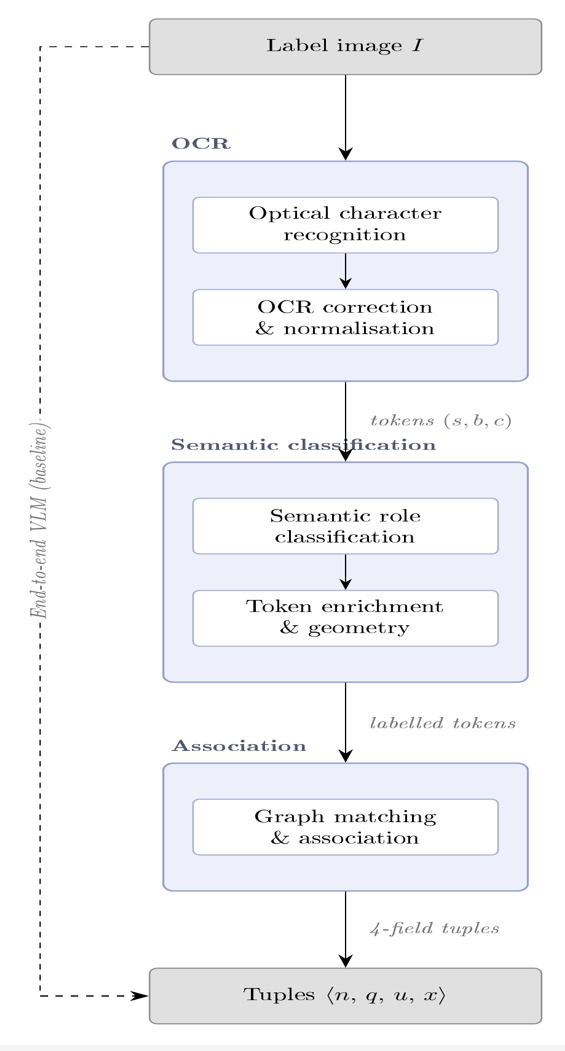
\includegraphics[width=\linewidth,height=0.80\textheight,keepaspectratio]{pipeline_overview.png}
  \caption[Pipeline overview]{%
    Overview of the proposed OCR-guided extraction pipeline. The input label image is first converted into OCR tokens, which are then corrected, classified, enriched with layout information, represented in a semantic graph, and finally associated into structured nutrient tuples. The figure also shows the main ablation points evaluated in the experiments: the OCR engine, the semantic classifier, and the association engine. The dashed branch represents the end-to-end vision--language baseline, which bypasses the modular OCR-guided pipeline.}
  \label{fig:pipeline-overview}
\end{figure}

\subsection{Ablation axes and experimental design}\label{sec:overview-ablation}

Because the pipeline is modular, the experiments are designed to test the effect of changing one stage at a time. The thesis focuses on three main ablation axes: the OCR engine, the semantic classifier, and the association engine. In addition, an end-to-end vision--language model is included as an external baseline, since it follows a different extraction strategy and does not use the modular OCR-guided pipeline.

The first ablation axis is the OCR engine. EasyOCR and PaddleOCR PP-OCRv5 are compared while keeping the remaining stages of the pipeline fixed. This comparison is performed first because OCR quality directly affects all later stages of the pipeline. The OCR engine selected from this experiment is then used in the remaining ablation experiments.

The second ablation axis is the semantic classifier. Three classifier variants are compared: the rule-based classifier, the BGE-M3 embedding classifier with cosine similarity, and the GLiNER-biomed classifier. These variants are included because they represent different design trade-offs. The rule-based classifier is fast and transparent, but depends on the coverage of the manually defined lexicon. The embedding classifier is more flexible with unseen surface forms, but can introduce semantic confusion when visually or semantically similar tokens are close together. GLiNER provides a different pre-trained zero-shot alternative, with behaviour that differs from both the rule-based and embedding-based approaches.

The third ablation axis is the association engine. The first variant uses the simpler graph constructor and traversal strategy, referred to as graph~v1. The second variant uses the geometry-aware graph constructor and traversal strategy, referred to as graph~v2. The third variant replaces graph traversal with a vision--language model association step based on an injected token table. In this VLM-association variant, the model receives the corrected token table before C15 normalisation, and C15 is applied afterwards to the model output.

After the OCR engine is fixed, the classifier and association axes are combined in a \(3 \times 3\) factorial experiment. In other words, each semantic classifier is evaluated with each association engine. The end-to-end vision--language baseline is evaluated separately, since it maps the original label image directly to output tuples and does not use the OCR-guided graph pipeline. This baseline is included to compare the proposed modular and interpretable design with a more direct black-box alternative.

One implementation detail is important for reading the experimental results. The enrichment stage is executed for all pipeline configurations, but graph~v1 does not use the enriched structural attributes. It relies only on the raw token geometry. Graph~v2, in contrast, uses the enriched token information when constructing edges. Therefore, although enrichment is present in the pipeline, not every association engine benefits from it in the same way. This distinction helps explain the performance difference between graph~v1 and graph~v2 in the experiments chapter.

The full experiment matrix, dataset description, evaluation metrics, and tuple-matching procedure are described in Chapter~\ref{chap:evaluation}. The quantitative results and ablation comparisons are reported in Chapter~\ref{chap:experiments}.

\begin{table}[htbp]
  \centering
  \caption[Implementation names and the names used in the text]{Mapping between the implementation (Python) names in the codebase and the plain-language names used in this chapter. The text uses the right-hand names; the left-hand names are listed only so each term can be traced back to the code. Model identifiers (\mcode{BAAI/bge-m3}, \mcode{Ihor/gliner-biomed-bi-large-v1.0}) and canonical output values (\mcode{per_100g}, \mcode{per_serving}, \mcode{per_daily_dose}, \mcode{per_100ml}, \mcode{nrv_percent}, \mcode{serving_size}) are kept verbatim in the text, because they are the exact strings the system reads or emits.}
  \label{tab:impl-names}
  \small
  \begin{tabular}{@{}ll@{}}
    \toprule
    \textbf{Implementation name} & \textbf{Name used in the text} \\
    \midrule
    \multicolumn{2}{@{}l}{\emph{Pipeline modules}}\\
    \mcode{paddleOCR_corrector_v2.py} & OCR corrector \\
    \mcode{token_enricher.py}         & token enricher \\
    \mcode{geometry_engine.py}        & geometry engine \\
    \mcode{graph_constructor.py}      & graph-v1 constructor \\
    \mcode{graph_constructor_v2.py}   & graph-v2 constructor \\
    \mcode{association_v2.py}         & graph-v2 associator \\
    \addlinespace
    \multicolumn{2}{@{}l}{\emph{Graph~v1 edge types}}\\
    \mcode{SAME_ROW}      & same-row edge \\
    \mcode{SAME_COL}      & same-column edge \\
    \mcode{ADJACENT}      & adjacency edge \\
    \mcode{CONTEXT_SCOPE} & context-scope edge \\
    \addlinespace
    \multicolumn{2}{@{}l}{\emph{Graph~v2 edge types}}\\
    \mcode{ROW_COMPAT}      & row-compatibility edge \\
    \mcode{COL_COMPAT}      & column-compatibility edge \\
    \mcode{DIRECTIONAL_ADJ} & directional-adjacency edge \\
    \mcode{CONTEXT_SCOPE}   & context-scope edge \\
    \mcode{HEADER_SCOPE}    & header-scope edge \\
    \addlinespace
    \multicolumn{2}{@{}l}{\emph{Row-edge modes}}\\
    \mcode{overlap}      & vertical-overlap mode \\
    \mcode{cy}           & vertical-centre mode \\
    \mcode{role_rank}    & role-rank mode \\
    \mcode{role_rank_cy} & role-rank plus vertical-centre mode \\
    \addlinespace
    \multicolumn{2}{@{}l}{\emph{Column-edge modes}}\\
    \mcode{overlap}   & horizontal-overlap mode \\
    \mcode{cx}        & horizontal-centre mode \\
    \mcode{column_id} & column-identifier mode \\
    \addlinespace
    \multicolumn{2}{@{}l}{\emph{Overlap thresholds}}\\
    \mcode{row_overlap_min}     & minimum row overlap \\
    \mcode{col_overlap_min}     & minimum column overlap \\
    \mcode{context_overlap_min} & minimum context overlap \\
    \bottomrule
  \end{tabular}
\end{table}

% =====================================================================
%  4.2  OCR + CORRECTION
% =====================================================================
\section{Optical Character Recognition and Token Correction}\label{sec:ocr}

The first stage of the pipeline converts the input label image into text tokens. Although OCR is not the main contribution of this thesis, its quality has a direct impact on all later stages. If a nutrient name is missed, a quantity is read incorrectly, or a bounding box is inaccurate, the graph-based association stage receives incomplete or misleading evidence. For this reason, OCR is included as the first ablation axis in the experiments.

Two OCR engines are considered: EasyOCR and PaddleOCR PP-OCRv5~\cite{cui2025paddleocr}. Both engines are connected to the same token interface, so the downstream pipeline receives a consistent input format regardless of which OCR engine is used. Each detected token contains the recognised text, its bounding box, and the confidence score returned by the OCR engine.

\subsection{Text recognition}\label{sec:ocr-recognition}

Both OCR engines return a list of detected text regions, and each detection is mapped to the common token format \(t_i = (s_i, b_i, c_i)\) defined in Section~\ref{sec:overview-problem}. This shared format is what keeps the rest of the pipeline independent of the OCR engine.

EasyOCR is run once using a combined German--English setting~\cite{easyocr}. This setting is suitable for the dataset because many nutrition and supplement labels contain a mixture of German and English text. PaddleOCR PP-OCRv5 is run in a multi-pass configuration. One pass uses the English model, while a second pass uses the Latin model. The Latin model is useful for this task because it covers several European languages that appear on supplement labels, including German, French, Dutch, Italian, and Spanish.

After the two PaddleOCR passes, the outputs are merged. The detected tokens are first sorted by confidence, and a greedy intersection-over-union procedure is then used to remove duplicate detections. If a new token overlaps an already accepted token by more than \(0.50\) IoU, it is discarded, so the higher-confidence reading is kept. The remaining tokens are then sorted approximately from top to bottom and from left to right. This ordering is used only as a convenient token order; the later graph-based stages still rely primarily on token geometry rather than on the OCR output sequence.

The purpose of the second PaddleOCR pass is to improve recall. On mixed-language labels, a single OCR language model may miss tokens that fall outside its strongest language coverage. This is especially important in the present task because missing one nutrient name, quantity, or unit can prevent an entire tuple from being reconstructed.

No confidence threshold is applied directly after OCR. Instead, all recognised tokens are passed to the later stages, including tokens with low confidence. The decision about whether a token is useful, noisy, or irrelevant is delayed until semantic classification. This avoids removing potentially important tokens too early, especially when a low-confidence OCR result still contains a relevant nutrient name, quantity, or unit.

\subsection{Token correction and normalisation}\label{sec:ocr-correction}

The raw OCR output still contains several errors that are common in dense nutrition and supplement labels. Values may be fused with their units, such as \texttt{250mg}. Unit characters may also be misread, for example \texttt{m9} instead of \texttt{mg}. In some cases, reference-value percentages are attached to the quantity, as in \emph{0,44mg(88\%)}. Nutrient names may also be split across multiple OCR tokens, or they may appear in different languages on the same label.

The correction stage addresses these recurring OCR problems before semantic classification. Its purpose is not to rewrite the OCR output freely, but to apply narrow and traceable corrections. Tokens that do not match any correction rule are left unchanged. This is important because overly aggressive correction can introduce new errors. For each modified token, the correction stage can keep the original text, the corrected text, and the identifiers of the rules that were applied. This makes the correction process easier to inspect during error analysis.

The correction process consists of two main parts. The first part operates on individual tokens. It removes border artefacts, normalises decimal separators, fixes common unit glyph errors, detects fused context headers, and splits tokens where a quantity and a unit have been recognised as one string. The second part operates on the full token list. It handles cases where a nutrient name is split across neighbouring tokens or continues on the next line, and it applies the final nutrient-name normalisation.

The order of the correction rules is important. Simple surface repairs are applied first, such as removing border characters and normalising decimal commas. Unit repairs are then applied before quantity--unit splitting. Context headers are detected early, because a token such as \texttt{pro 100g} should not be treated in the same way as a nutrient quantity. Only after these checks are the value-splitting rules applied.

One of the most important correction rules is the fused quantity--unit split. If a token consists exactly of a number followed by a unit, such as \texttt{250mg}, it is split into a quantity token and a unit token. The original bounding box is divided according to the character lengths of the two parts, so both new tokens keep approximate spatial positions. Protected context expressions, such as \texttt{100g} and \texttt{100ml}, are not split because they usually describe a reference column rather than a nutrient value.

Another important rule removes trailing reference-value percentages. For example, \texttt{0,44mg(88\%)} is first reduced to \texttt{0,44mg}, which can then be split into a quantity and a unit. This prevents the percentage from being absorbed into the quantity field.

The post-processing rules operate on relationships between tokens. If a nutrient name is split across adjacent tokens on the same row, the tokens can be merged. A similar rule handles nutrient names that continue on the following line. Another guarded rule separates a unit that has been absorbed into a nutrient or header token. Finally, the C15 normalisation rule maps nutrient names to the canonical English forms used in the annotation schema. For example, \texttt{Eiwei{\ss}} is normalised to \texttt{Protein}, and \texttt{davon Zucker} is normalised to \texttt{Sugars}. This rule leaves numbers, units, and context headers unchanged.

In the graph-based pipeline, C15 is applied as the final normalisation step before tuple construction and evaluation. In the VLM association path, however, C15 is applied after the model output. This is because the VLM receives the corrected token table before C15 normalisation, and the predicted tuples are then normalised to the same canonical forms used in the evaluation.

Some correction ideas were implemented during development but disabled in the evaluated configuration. The trailing-digit artefact heuristic, C4/C5, was disabled because it produced too many false positives on real label images. The energy-pair splitter, C18/C18b, which separates a fused \texttt{kJ/kcal} cell into two energy quantities, was also implemented but is not active in the final evaluated setup. Both are retained in the codebase but excluded from the reported pipeline configuration.

Table~\ref{tab:correction-rules} summarises the active correction rules and their purpose.

\begin{table}[ht]
  \centering
  \caption[OCR correction rules]{Active OCR correction rules used before semantic classification. Per-token rules operate on individual OCR tokens, while post-pass rules operate on relationships between tokens. C4/C5 and C18/C18b were implemented during development but are not active in the evaluated configuration.}
  \label{tab:correction-rules}
  \small
  \begin{tabular}{@{}llp{0.60\linewidth}@{}}
    \toprule
    \textbf{Rule} & \textbf{Phase} & \textbf{Purpose} \\
    \midrule
    C1 & per-token & Normalises decimal separators by converting commas or apostrophes between digits into a dot, for example \texttt{0,8} to \texttt{0.8}. \\

    C2/C3 & per-token & Splits a token that consists exactly of a number followed by a unit into a quantity token and a unit token. Protected context headers such as \texttt{100 g} and \texttt{100 ml} are exempt. \\

    C6 & per-token & Splits a fused energy label and unit, for example \texttt{ENERGIEkJ/kcal} into \texttt{ENERGIE} and \texttt{kJ/kcal}. \\

    C7 & per-token & Normalises fused context headers, such as \texttt{PRO100g} to \texttt{pro 100g} and \texttt{PER100ML} to \texttt{per 100ml}. Tokens recognised as context headers are protected from value splitting. \\

    C8/C9 & per-token & Repairs common unit glyph errors, such as \texttt{Ug} or \texttt{ug} to $\mu$g, \texttt{m9} to \texttt{mg}, and \texttt{pg} to $\mu$g. \\

    C10 & per-token & Removes border artefacts such as \texttt{|}, \texttt{\{}, \texttt{\}}, \texttt{[}, \texttt{]}, and \texttt{\textbackslash} from token edges. If the token becomes empty, it is discarded. \\

    C11 & per-token & Fuzzy-matches corrupted nutrient names to canonical lexicon entries when the similarity is at least \(0.80\) and the token length is at least five characters. \\

    C12 & per-token & Applies targeted regular-expression repairs for corrupted numbers, units, and selected nutrient names, including corrupted forms of Magnesium. \\

    C13 & per-token & Splits compound energy values, for example \texttt{1625 kJ/383kcal} into separate quantity and unit tokens. \\

    C14 & post-pass & Merges a nutrient name that was split across adjacent tokens on the same row. \\

    C14b & post-pass & Merges a nutrient name that continues on the following line. \\

    C15 & post-pass & Normalises nutrient names to the canonical English forms used in the gold schema, such as \texttt{Eiwei{\ss}} to \texttt{Protein} and \texttt{davon Zucker} to \texttt{Sugars}. \\

    C16 & per-token\textsuperscript{\dag} & Removes a trailing reference-value percentage before quantity--unit splitting, for example \texttt{0,44mg(88\%)} to \texttt{0,44mg}. \\

    C17 & post-pass & Splits a unit that has been absorbed into a nutrient or header token, under a guard that restricts the rule to safe header names. \\
    \bottomrule
  \end{tabular}

  \vspace{0.5em}
  \raggedright
  \textsuperscript{\dag}\,C16 is applied inside the C2/C3 splitting routine.
\end{table}

% =====================================================================
%  4.3  SEMANTIC ROLE CLASSIFICATION
% =====================================================================
\section{Semantic Role Classification}\label{sec:classifier}

Once the OCR output has been corrected, the pipeline contains a cleaner list of tokens, but these tokens are still only pieces of text with positions. At this point, the pipeline has not yet determined whether a token is a nutrient name, a quantity, a unit, a phrase that provides context (such as ``per 100~g''), or simply text that should be ignored. The role-classification stage adds this layer of meaning before the tokens are used to build the graph.

This stage is treated as the second ablation axis because the difficulty of classification is not the same for all roles. Some categories have relatively stable surface forms. Numerical values, units, NRV percentages, and many context expressions can often be recognised using deterministic patterns. For instance, tokens such as \texttt{250}, \texttt{mg}, or \texttt{per 100g} usually provide strong clues about their role. Nutrient names, however, are less predictable. They may appear in different languages, use different surface forms, or be distorted by OCR errors.

For this reason, the classification step is organised as a hybrid process. A deterministic cascade is first used for roles that can be identified from clear textual patterns, such as quantities, units, NRV values, context expressions, and noise. The remaining and more difficult decision is whether a token should be treated as a nutrient. This nutrient-detection step is where the three classifier variants differ in the experimental design.

All three classifier variants share the same deterministic cascade. They differ only in the final nutrient-detection step, where the system decides whether a remaining candidate should be treated as a nutrient. The three variants evaluated in this thesis are the rule-based lexicon classifier, the BGE-M3 embedding classifier, and the GLiNER-biomed classifier. Since none of these variants is trained on the target label dataset, the classification stage remains zero-shot in the sense defined in Section~\ref{sec:overview-problem}. Figure~\ref{fig:classifier-ablation} shows this ablation axis: the upstream and downstream stages are held fixed, and only the nutrient/not-nutrient classifier is exchanged.

\begin{figure}[htbp]
  \centering
  \IfFileExists{classifier_ablation.png}{%
    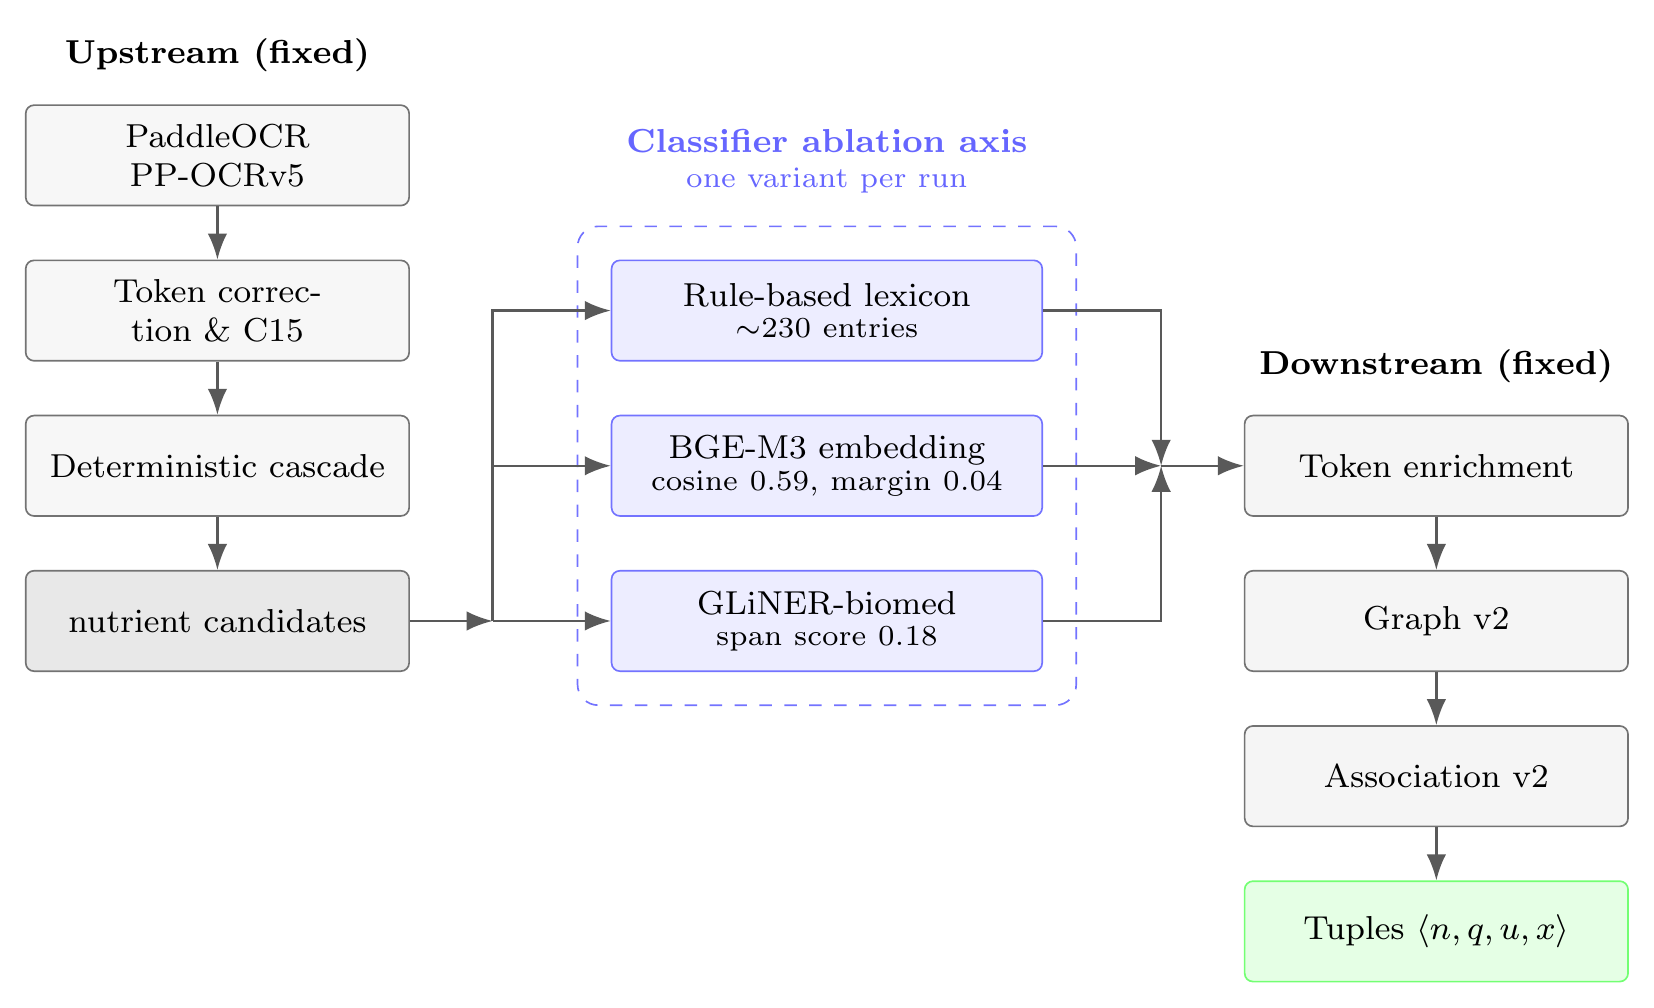
\includegraphics[width=\linewidth]{classifier_ablation.png}%
  }{%
    \fbox{\parbox[c][42mm][c]{0.92\linewidth}{\centering\itshape
      Classifier-ablation figure placeholder. Replace with
      \texttt{classifier\_ablation.png}.}}%
  }
  \caption[The semantic-classifier ablation axis]{%
    The semantic-classifier ablation axis. The upstream stages (PaddleOCR PP-OCRv5, token correction including C15, and the deterministic cascade) and the downstream stages (token enrichment, graph~v2 construction, and association~v2) are held fixed. Only the nutrient/not-nutrient decision is exchanged between the rule-based lexicon classifier, the BGE-M3 embedding classifier, and the GLiNER-biomed classifier. Exactly one classifier variant is active in any single experiment run.}
  \label{fig:classifier-ablation}
\end{figure}

\subsection{The deterministic cascade}\label{sec:classifier-cascade}

The deterministic cascade assigns roles to corrected tokens through an ordered sequence of checks. For each token, the first matching rule determines the role. This ordering is important because some tokens may satisfy more than one pattern.

The cascade first checks for short unit tokens, such as \texttt{g} or \texttt{l}. These are handled early because the correction stage may split fused values into a quantity and a short unit token. If these units were checked later, they could be mistakenly removed as noise.

The next role handled is \textsc{nrv}. This captures reference-value percentages such as \texttt{80\%} or \texttt{100\% NRV}. These values are useful for preserving label information, but they are not part of the main four-field tuple.

Context expressions are then detected and normalised. Tokens that match the context map are assigned the role \textsc{context} and mapped to canonical forms such as \texttt{per\_100g}, \texttt{per\_serving}, or \texttt{per\_daily\_dose}. Serving-size expressions are also treated as context information because they define the basis under which a quantity should be interpreted.

After the context checks, the cascade handles noise, unit-lexicon matches, and numeric quantities. Noise includes residual artefacts and isolated characters that do not provide useful information for tuple construction. Tokens that match the unit lexicon are labelled as \textsc{unit}. Numeric tokens, including integers, decimals, and comparator-prefixed values such as \texttt{<0.1}, are labelled as \textsc{quantity}.

If a token reaches the end of the cascade, it has not been recognised as a percentage, context expression, unit, quantity, or noise. At this point, it is treated as a nutrient candidate and passed to the nutrient/not-nutrient decision step. The OCR confidence remains attached to the token, but it is not used as a hard filter, since a low-confidence token may still contain useful nutritional information.

The auxiliary roles are handled differently during evaluation. The \textsc{nrv} role corresponds to the \texttt{nrv\_percent} field and is kept as additional information, but it is not part of the headline four-field score. Serving-size information is folded into \textsc{context}, because it defines the reference condition under which a nutrient quantity is reported.

\subsection{The lexicon node: rule-based classifier}\label{sec:classifier-rule}

The rule-based classifier decides whether a nutrient candidate should be assigned the role \textsc{nutrient} by checking it against a curated nutrient lexicon. The lexicon contains roughly 230 entries and covers several languages that appear in the dataset, including German, English, French, Dutch, Italian, and Spanish.

The classifier first attempts a direct lexicon match. If no exact match is found, it applies a small set of supporting heuristics. These include substring matching for longer nutrient names, tokens that begin with \texttt{vitamin}, shorthand vitamin forms such as \texttt{B12}, multilingual slash-separated forms such as \texttt{Fett / fat}, and cases where a unit has been attached to the nutrient name. For example, a token such as \texttt{energie kj} can be reduced to \texttt{energie} before the lexicon check is applied. If none of these checks succeeds, the candidate remains labelled as \textsc{unknown}.

The main advantage of this classifier is that it is fast, transparent, and easy to inspect. It also performs well when the nutrient appears in a form covered by the lexicon or one of the supporting rules. Its main limitation is coverage. Nutrient names that are missing from the lexicon, written in an unexpected form, or heavily corrupted by OCR may not be recognised. Improving this classifier therefore requires manual lexicon extension, often across several languages. This limitation motivates the comparison with the embedding-based and GLiNER-based variants.

\subsection{The embedding node: BGE-M3}\label{sec:classifier-embedding}

The embedding classifier keeps the deterministic cascade unchanged, but replaces the final lexicon-based nutrient decision with a semantic similarity test. It uses the pre-trained multilingual encoder \texttt{BAAI/bge-m3}~\cite{chen2024bgem3}. Instead of training a classifier on the target label dataset, the method represents nutrient and non-nutrient categories through short prototype phrases and compares candidate tokens to these prototypes in the embedding space.

The main positive category is \textsc{nutrient}. To avoid treating every semantically meaningful token as a nutrient, the classifier also defines non-nutrient categories as negative anchors. For each category, the candidate is compared with the corresponding prototypes, and the highest cosine similarity is used as the category score.

A candidate is not encoded only as an isolated word. Instead, it is encoded together with a small amount of row context. Tokens are grouped with nearby row neighbours using vertical-centre proximity, and the combined text is passed to the encoder. For example, a token such as \texttt{Fett} may be encoded together with nearby values as \texttt{Fett 12.5 g}. This gives the encoder more information, because a word appearing next to a quantity and unit is more likely to be part of a nutrient row.

The candidate is accepted as \textsc{nutrient} only if two conditions are met. First, its similarity to the nutrient prototypes must exceed the acceptance threshold. Second, this score must be higher than the best non-nutrient score by a defined margin. If either condition fails, the token remains \textsc{unknown}.

The embedding node can be used in two modes. In the embedding-only mode, all nutrient candidates are decided by the encoder, without using positive lexicon decisions. In the hybrid mode, the lexicon classifier keeps its positive nutrient matches, and the embedding model is used only to recover candidates that the lexicon left as \textsc{unknown}.

\subsubsection{Threshold calibration}

The embedding node uses two decision parameters: the cosine similarity threshold for accepting a token as a nutrient, and the margin over the best non-nutrient category. These parameters were selected through a token-level grid search over nutrient-candidate decisions. The calibration set contained 796 candidate decisions from the 57 label images, including 462 true nutrient tokens and 334 non-nutrient tokens.

For each threshold--margin combination, every candidate was classified either as \textsc{nutrient} or not, and the prediction was compared with the manual token-level label. Figure~\ref{fig:threshold-sweep} shows the threshold sweep for the embedding node. The best operating region was found around a cosine threshold of \(0.59\), where the token-level nutrient-classification F1 score reached approximately \(0.87\).

The margin parameter had a smaller effect than the acceptance threshold. Strong configurations generally used a small margin, usually between \(0.01\) and \(0.07\). Larger margins made the classifier more conservative, but also removed many correct nutrient names because some true nutrients still had moderate similarity to non-nutrient prototypes. Based on this sweep, the final embedding configuration uses a cosine threshold of \(0.59\) and a margin of \(0.04\).

\begin{figure}[htbp]
  \centering
  \IfFileExists{threshold_sweep.png}{%
    
\includegraphics[width=\linewidth]{threshold_sweep.png}%
  }{%
    \fbox{\parbox[c][42mm][c]{0.92\linewidth}{\centering\itshape
      BGE-M3 calibration heatmap placeholder. Replace with
      \texttt{threshold\_sweep.png}.}}%
  }
  \caption[Threshold calibration of the BGE-M3 nutrient node]{%
    Threshold--margin calibration for the BGE-M3 nutrient node. The heatmap shows token-level F1 scores across cosine similarity thresholds and margins. The black circle marks the best setting (threshold \(0.59\), margin \(0.04\); F1 = \(0.869\)), and the red cross shows the default setting (\(0.40\), \(0.10\)).}
  \label{fig:threshold-sweep}
\end{figure}


\subsection{The GLiNER node: GLiNER-biomed}\label{sec:classifier-gliner}

The third classifier variant uses GLiNER-biomed, specifically \emph{Ihor/gliner-biomed-bi-large-v1.0}~\cite{yazdani2025glinerbiomed}. Here, the model is used as a zero-shot named-entity recogniser. This means that it can receive an entity description at inference time and identify matching spans without being trained on the target supplement-label dataset.

In the proposed pipeline, the remaining nutrient candidates are passed to GLiNER using one descriptive entity label: \texttt{nutritional ingredient or vitamin or mineral}. If a candidate is covered by an accepted span for this label, it is assigned the role \textsc{nutrient}. Otherwise, it remains \textsc{unknown}. The bi-large version is used because it provided stronger zero-shot recall and more stable behaviour on German OCR text than smaller alternatives during development.

\subsubsection{Threshold calibration}

In this setup, GLiNER has one main decision parameter: the span-acceptance threshold. This threshold controls how confident the model must be before a detected span is accepted as evidence for a \textsc{nutrient} label. Unlike the BGE-M3 embedding node, the GLiNER node does not use a margin against non-nutrient categories.

The threshold was selected using the same token-level calibration approach used for the embedding classifier. Each nutrient candidate from the 57 label images was scored by GLiNER, and the predictions were compared with the manual token-level labels. Precision, recall, and token-level nutrient-classification F1 were then computed across the threshold grid. Figure~\ref{fig:threshold-sweep-gliner} shows the resulting curve for 803 candidates, consisting of 438 true nutrients and 365 non-nutrients.

The selected threshold is \(0.18\). At this operating point, the token-level nutrient-classification F1 is approximately \(0.89\), with precision \(0.91\) and recall \(0.87\). The threshold is deliberately kept relatively low because the later graph-based association stage can still reject some incorrectly connected candidates, while a nutrient missed at the classification stage cannot be recovered later.

\begin{figure}[htbp]
  \centering
  \IfFileExists{threshold_sweep_gliner_c15.png}{%
    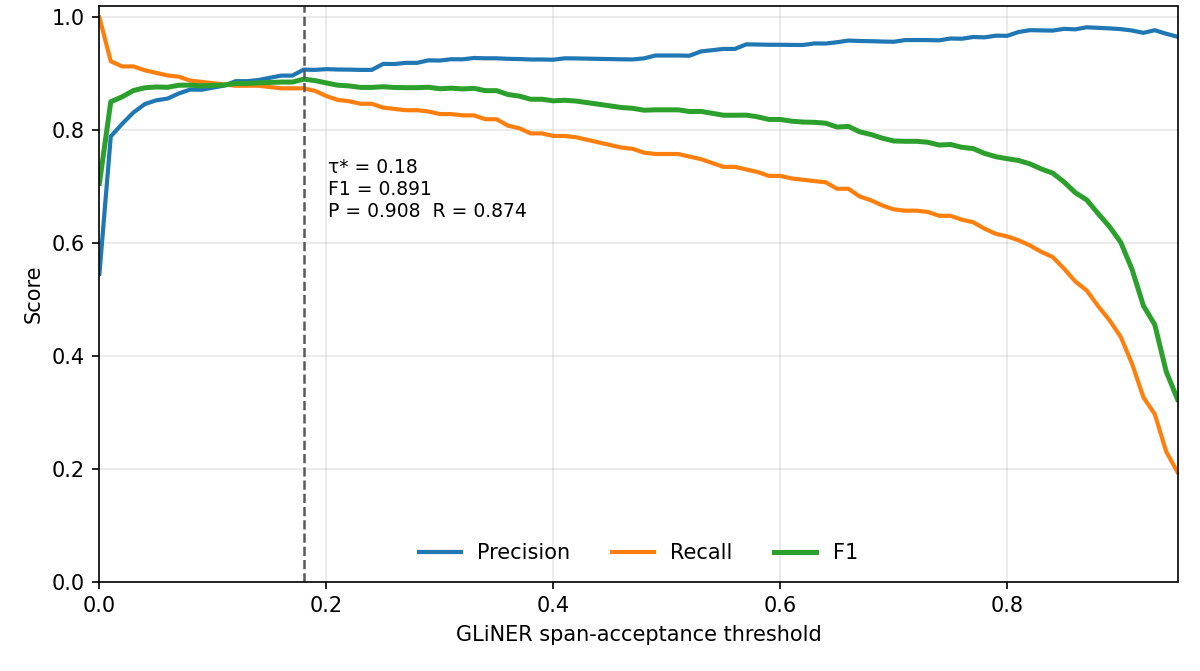
\includegraphics[width=\linewidth]{threshold_sweep_gliner_c15.png}%
  }{%
    \fbox{\parbox[c][42mm][c]{0.92\linewidth}{\centering\itshape
      GLiNER threshold-sweep placeholder. Replace with
      \texttt{threshold\_sweep\_gliner\_c15.png}.}}%
  }
  \caption[Threshold calibration of the GLiNER nutrient node]{%
    Threshold calibration for the GLiNER nutrient node. The plot shows precision, recall, and token-level nutrient-classification F1 across different span-acceptance thresholds, using 803 nutrient-candidate decisions from the 57 label images. The selected threshold is \(0.18\), which gives a token-level F1 of approximately \(0.89\), with precision \(0.91\) and recall \(0.87\).}
  \label{fig:threshold-sweep-gliner}
\end{figure}


\subsection{Choice of classifier}\label{sec:classifier-choice}

The three classifier variants were included because they represent different design choices. The rule-based classifier is the easiest to inspect and is very effective when the nutrient name is covered by the lexicon. Its limitation is that it remains a closed-vocabulary approach. A new nutrient name, spelling variant, or heavily corrupted OCR token can only be recognised if it is already covered by the lexicon or by one of the supporting rules.

The embedding classifier is less dependent on exact lexical coverage. By comparing candidate tokens with nutrient prototypes in the embedding space, it can sometimes recover nutrient names that are missing from the lexicon. However, this flexibility also introduces a risk. Tokens that are semantically related to nutrition, but are not nutrient names, may receive high similarity scores.

GLiNER provides a third alternative. It does not require a manually curated nutrient lexicon, but it can still detect nutrient-like spans from a descriptive entity label. This makes it useful for the generalisation argument of the thesis, because the classifier can be applied without training on the target label dataset and without manually adding every possible nutrient name. In the experiments, GLiNER gives performance close to the strongest classifier settings while remaining a pre-trained zero-shot component.

For this reason, the GLiNER node is treated as the main zero-shot classifier configuration in the later analysis. The embedding node is kept as a second zero-shot alternative, while the rule-based classifier is kept as a strong and transparent closed-vocabulary reference. All three classifiers are still included in the full classifier-by-association experiment matrix reported in Chapter~\ref{chap:experiments}.
% =====================================================================
%  4.4  TOKEN ENRICHMENT AND GEOMETRY
% =====================================================================

\section{Token Enrichment and Geometry}\label{sec:enrichment}

After the tokens have been classified, the pipeline knows what type of information each token may contain, but it still does not know how these pieces of information belong together on the label. A token can be marked as a nutrient, a quantity, a unit, or a context expression, but this label alone does not reveal its layout relationship to the other tokens. For example, it does not tell whether two tokens are part of the same row, whether a value belongs to a particular column, or whether a header controls the interpretation of the values beneath it. The enrichment stage is introduced to add this missing layout structure before the graph is built.

This stage extends each non-noise token with additional information that is not available from the classifier alone. Part of this information is geometric, such as the token position and its distance from nearby tokens. Another part is structural, such as the estimated row, column, column role, header status, and ordinal position within a column. These attributes are later used by the graph constructor to decide which tokens should be connected and what type of relationship each connection represents.

\subsection{Direction-aware geometry}\label{sec:enrichment-geometry}

The geometry engine does not rely only on the rectangular position of a token. Instead, it also estimates the local text direction around each token. This is particularly useful for supplement labels because the images are not always captured under ideal conditions. Labels may be slightly rotated, photographed from an angle, or printed on curved packaging, making purely axis-aligned geometric reasoning unreliable. By estimating a direction vector that follows the reading direction of each token and using this vector when comparing neighbouring tokens, the pipeline can distinguish movement along a row from movement across rows and therefore infer spatial relationships more reliably under these conditions.

For each token, the engine estimates its centre point \((c_x, c_y)\), local text angle, a direction vector along the reading direction, and a normal vector perpendicular to it. When a four-corner polygon is available, it is used for this estimation; otherwise, the token bounding box is used. This gives the pipeline a local coordinate system for comparing tokens. Movement along the direction vector roughly corresponds to movement within the same row, while movement along the normal vector corresponds more closely to movement between rows.

Two tokens are considered to belong to the same row if they point in nearly the same direction and are close to each other. The system allows small differences in angle (about \(15^\circ\)). Columns are found in a similar way, but using the other direction. This helps the system still work well even if the label is slightly rotated or photographed at an angle.

Rows and columns are then assigned using several layout modes. In the centre-coordinate (\(c_x/c_y\)) mode, a gap-based grouping strategy is used: after projecting and sorting the tokens, the algorithm starts a new row or column whenever the gap between consecutive tokens becomes too large. At the reference resolution, the row gap along the \(y\)-axis is about \(25\) pixels, while the column gap is about \(60\) pixels, and these thresholds are scaled according to the image size. Other modes are also supported, including overlap-based grouping and role-rank strategies, which use different criteria to determine row and column membership depending on the label structure.

\subsection{Structural attributes}\label{sec:enrichment-structure}

Once the approximate rows and columns have been identified, the token enricher adds a structural description to each token. This description goes beyond the token's text and position. Each token is assigned a row identifier and a column identifier, which allows the later stages to reason about the table-like structure of the label.

The columns are then interpreted using the semantic roles of the tokens they contain. For example, if most non-header tokens in a column are nutrient names, the column is treated as a nutrient-name column. If a column mainly contains numerical values, it is treated as a value column. Other columns may be interpreted as unit columns or NRV columns. This column-level information helps the graph constructor distinguish between different parts of the label instead of relying only on local token proximity.

The enrichment stage also identifies header tokens and uses them to assign context information to value columns. This is important because many nutrition and supplement labels report the same nutrients under more than one basis. For example, one column may give values per serving, while another column may give values per 100~g, per 100~ml, or per daily dose. To keep these value columns separate, the enricher can assign a dosage-stream identifier to each context-bearing value column. In this way, the graph stage can treat different value columns as separate streams rather than mixing quantities that belong to different contexts.

Several rank-based attributes are also computed. Each token receives a rank within its row, a rank within its column, and a role-specific rank. The column rank is calculated over non-header tokens, while the role-specific rank is calculated separately for roles such as \textsc{nutrient}, \textsc{quantity}, and \textsc{unit}. These ranks are not the main mechanism for association, but they provide useful fallback information and allow alternative edge-construction modes to be tested in the graph stage.

The enriched tokens also keep confidence values for row and column membership. This is useful because the layout is not always clear. Some labels have irregular spacing, weak table boundaries, or mixed paragraph-and-table formatting, so assigning a token to a row or column may be uncertain.

The enricher assumes that the main nutritional information in an image is mostly contained in one table-like region. This assumption fits most labels in the dataset, but it is still a simplification. When a label contains multiple separate tables, or when table entries are mixed with paragraph text, some structural attributes may become less reliable. For this reason, the graph stage does not depend only on the induced table structure. It also keeps geometric relations and fallback routes, which makes the association process more robust when the structural enrichment is imperfect.

\subsection{Two views of the row relation}\label{sec:enrichment-rowviews}

The row relation is one of the most important layout cues for tuple reconstruction. In many nutrition and supplement tables, a nutrient is associated with a quantity simply because both appear on the same printed row. The enrichment stage therefore provides two ways to describe this relation before the graph is built.

The first view is geometric. Two tokens are considered related when they are aligned in the image. On clean labels, this can be approximated by comparing their \(c_y\) positions. A more robust criterion is to consider the extent they share along the vertical axis: tokens whose vertical spans have a large common extent are likely to belong to the same row, even when their heights differ. This criterion remains effective even when the label contains moderate distortions or variations in token size. In all cases, the row relation is derived directly from the visual layout of the label.

The second view is structural. Instead of relying only on pixel alignment, this view uses the ordinal order of tokens inside their columns. For example, the first nutrient can be paired with the first quantity, the second nutrient with the second quantity, and so on. This can work well when the columns are correctly detected and when the entries in each column follow the same order. In such cases, ordinal rank provides another way to recover the row relation, even if the visual alignment is not perfectly clean.

In practice, the structural view is more fragile than it may first appear. OCR errors can easily disturb the one-to-one ordering between nutrient, quantity, and unit columns. If a token is missed, one column becomes shorter than the others. If a quantity and unit are fused into one token, the expected unit sequence may change. Extra tokens, such as NRV percentages, footnote markers, or OCR artefacts, can also shift the rank count. The same problem can occur when the column detection itself is imperfect and the rank is computed over the wrong group of tokens.

Once the ordering is shifted, the error can propagate through the rest of the table. For example, if one quantity is missing near the top of a value column, the nutrients below it may be matched with quantities from neighbouring rows. This is particularly harmful for the quantity field, because quantities usually differ from row to row. Unit values, on the other hand, may still appear correct even when the row association is wrong, since many nutrients share repeated units such as \texttt{mg}. For this reason, a high unit score under rank-based pairing does not necessarily prove that the row matching itself is correct.

The geometric view is less sensitive to this type of OCR error. If one token is missing, fused, or falsely added, the remaining tokens still stay close to their printed row. A quantity that is visually aligned with a nutrient remains aligned, even if another entry above it is missing. Therefore, the graph uses geometric row edges as the main representation of the row relation, while ordinal ranks are kept only as fallback or experimental information. The edge-construction modes based on these two views are described in Section~\ref{sec:graph}, and their effect is evaluated in Chapter~\ref{chap:experiments}.

% =====================================================================
%  4.5  SEMANTIC GRAPH CONSTRUCTION
% =====================================================================
\section{Semantic Graph Construction}\label{sec:graph}

After the enrichment stage, each token carries more than just text. It now has a semantic role, geometric information, and structural attributes such as row or column membership. The next step is to represent these enriched tokens as a graph. The purpose of this graph is to make the possible relationships between tokens explicit before the final association step. Instead of searching over an unstructured list of OCR tokens, the matcher receives a graph that already indicates which tokens are likely to be aligned in the same row, belong to the same column, appear near each other, or fall under the same contextual scope.

In this graph, the nodes correspond to the non-noise tokens. The edges represent typed relationships between these tokens. These edges do not directly define the final output tuples, but they narrow and organise the search space for the association stage. For example, a row edge between a nutrient and a quantity suggests a possible nutrient--quantity relation. An adjacency or row edge between a quantity and a unit suggests a possible quantity--unit relation. Similarly, an edge from a context header to a value-bearing token can indicate the reference basis under which the value should be interpreted.

Two graph constructors are evaluated in this thesis. The first constructor, referred to as graph~v1, is the simpler variant. It builds relations using the classified tokens and their raw bounding-box geometry. The second constructor, graph~v2, uses the enriched representation described in Section~\ref{sec:enrichment}. This allows graph~v2 to use additional information such as row and column identifiers, column roles, ordinal ranks, dosage-stream identifiers, header flags, and direction-aware geometry. Figure~\ref{fig:graph-constructors} illustrates the difference between the two graph construction variants.

\begin{figure}[htbp]
  \centering
  \IfFileExists{graph_constructors.png}{%
    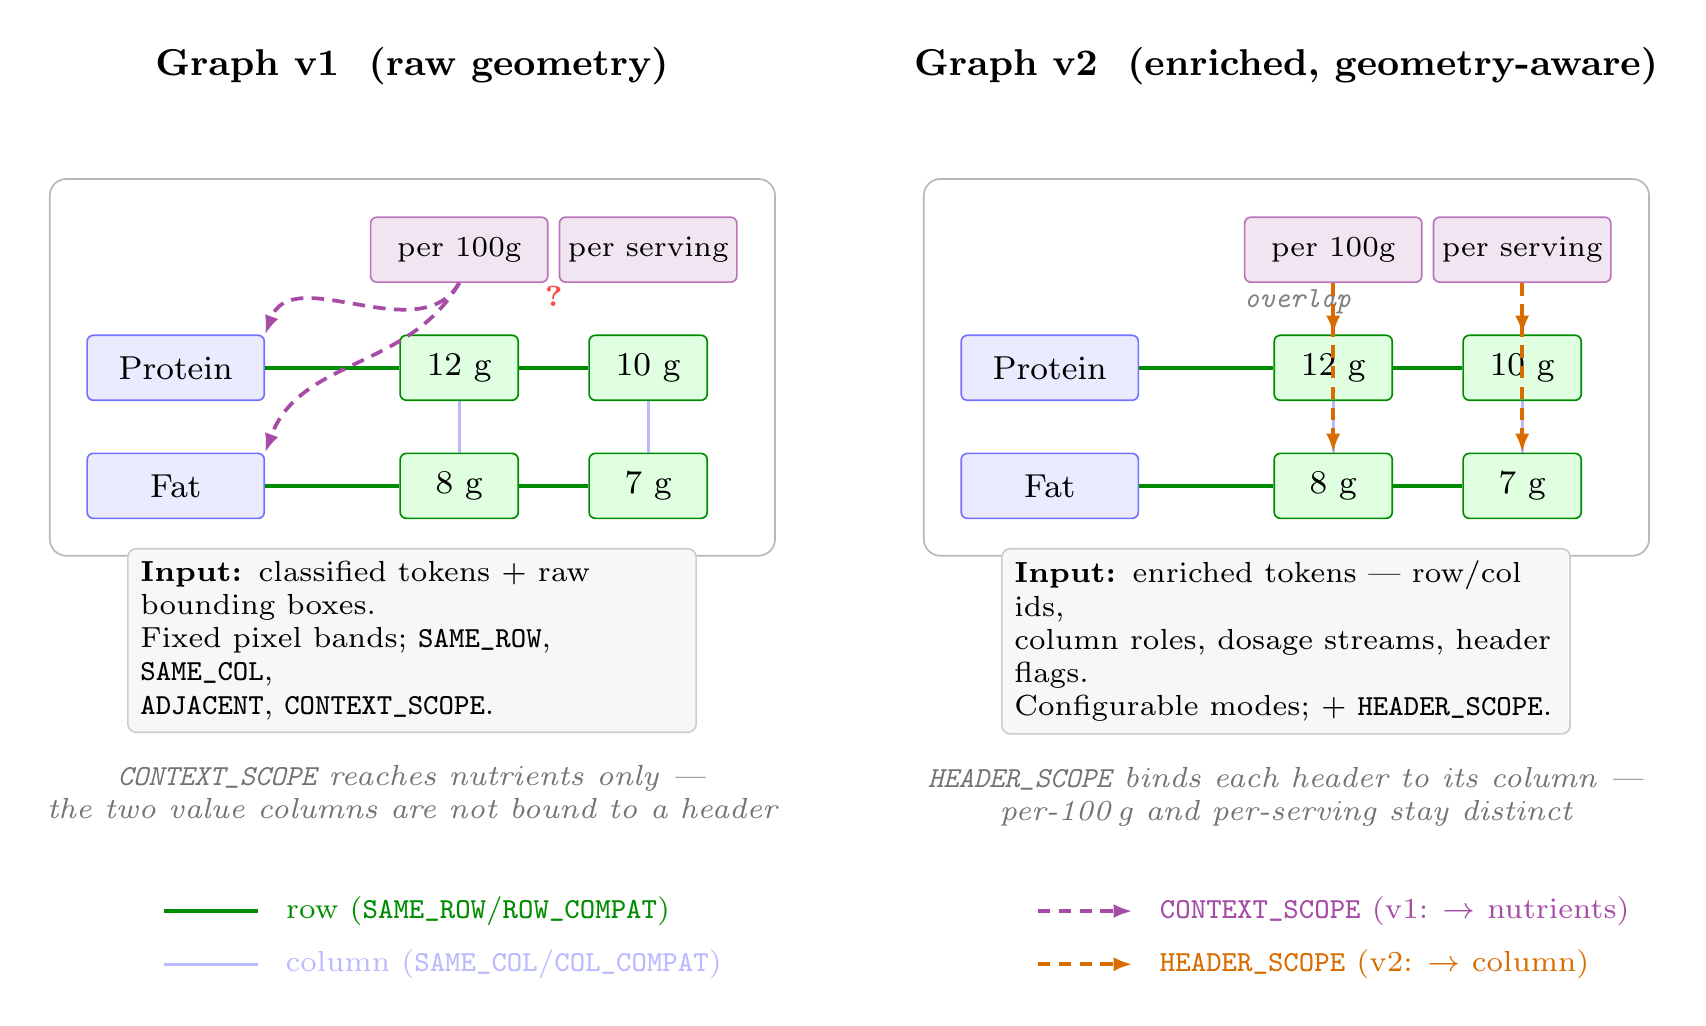
\includegraphics[width=\linewidth]{graph_constructors.png}%
  }{%
    \fbox{\parbox[c][52mm][c]{0.92\linewidth}{\centering\itshape
      Graph-constructor comparison figure placeholder. Replace with
      \mcode{graph_constructors.png}.}}%
  }
  \caption[Graph v1 and graph v2]{%
    Comparison of the two graph constructors on a label with two value columns. Graph~v1 builds edges from raw bounding-box geometry, and its context-scope edge edge reaches nutrient nodes only, so the two value columns are not bound to their respective headers. Graph~v2 uses the enriched token structure; its header-scope edge edge binds each header to the tokens in its own column, keeping the per-100\,g and per-serving contexts distinct.}
  \label{fig:graph-constructors}
\end{figure}

\subsection{Graph v1: the naive constructor}\label{sec:graph-v1}

Graph~v1 is used as the simple geometry-based baseline. It operates directly on the classified OCR tokens, without using the enriched representation described in Section~\ref{sec:enrichment}. Each non-noise token is converted into a graph node, and its centre point \((c_x, c_y)\) is recomputed from the token bounding box. The constructor therefore ignores the induced row and column identifiers, column roles, ordinal ranks, dosage streams, and header flags produced by the enrichment stage.

The edge set in graph~v1 is deliberately limited. It contains four main types of relations. The first is  same-row edge. This edge is added when two tokens have similar vertical centre positions, using a row band of approximately \(25\) pixels. The second relation is  same-column edge, which connects tokens whose horizontal centres are close to each other, using a narrower band of approximately \(20\) pixels.

The third relation is  adjacency edge. This edge is added when two token boxes are spatially close, with a distance threshold of approximately \(60\) pixels, and when no row or column edge has already been created between them. In practice, this relation acts as a fallback. For example, a unit may be slightly shifted away from its quantity because of OCR segmentation. Even if it does not satisfy the row or column criteria, it may still be recovered through an adjacency edge.

The fourth relation is context-scope edge. This is a directed edge from a context token to nutrient tokens below it, within a vertical range of approximately \(600\) pixels. The purpose of this edge is to allow a header or context phrase to influence the nutrient entries that appear underneath it.

All thresholds in graph~v1 are based on pixel distances, scaled according to the image height. This makes the constructor easy to understand and useful as a baseline, but it also limits its ability to represent the real structure of dense supplement labels. It treats the page mainly as a set of coordinates and does not use the table structure inferred during enrichment. As a result, graph~v1 cannot distinguish between different sources of row or column evidence. Its role in the experiments is therefore to show what can be achieved with simple geometric relations before adding the enriched structural information used in graph~v2.

\subsection{Graph v2: the geometry-aware constructor}\label{sec:graph-v2}

Graph~v2 uses the enriched token representation produced in the previous stage. Each node keeps the token text, semantic role, geometry, row and column identifiers, column role, ordinal ranks, dosage-stream identifier, and header flag. Unlike graph~v1, this constructor does not rely only on recomputing relations from the bounding boxes. Instead, it uses the layout and structural information already added during enrichment.

Because of this richer input, graph~v2 also defines a richer set of edge types. The main relations are  row-compatibility edge,  column-compatibility edge , directional-adjacency edge, context-scope edge, and header-scope edge. The main difference from graph~v1 is that row and column compatibility are no longer based on one fixed pixel-band rule. They can be created through different edge-construction modes, which makes it possible to compare geometric and structural interpretations of the label layout.

The row relation,  row-compatibility edge, can be built in several ways. The default mode is \mcode{overlap}. This is a geometric mode based on the shared vertical extent of two token boxes. Two tokens receive a row edge when the intersection of their vertical spans \([y_1, y_2]\) covers at least \(0.30\) of the shorter span. This threshold was selected by a coordinate-descent sweep over the three overlap thresholds, shown in Figure~\ref{fig:overlap-sweep}, in which the row threshold is the decisive axis while the column and context thresholds are nearly flat. The overlap criterion is more stable than comparing only the vertical centre points, because two tokens can still belong to the same printed line even when their bounding-box heights differ. A second geometric mode, vertical-centre mode, links tokens when the distance between their vertical centres is within a fixed band of approximately \(25\) pixels, although the effective tolerance depends on the resolution of the input image. Both geometric modes work as pairwise checks. Figure~\ref{fig:row-modes} contrasts the four row modes on a label where one quantity has been dropped by OCR.

The  role-rank mode mode is a structural mode that counts the order separately for each semantic role. In this mode, the \(k\)-th nutrient, the \(k\)-th quantity, and the \(k\)-th unit can be linked together. Since same-column links are allowed, this mode can recover some inline quantity--unit relations. However, it still depends on the ordinal sequence being correct, so it can fail when OCR errors shift the role-specific ranks.

The \mcode{role_rank_cy} mode combines the structural and geometric views. It creates a row edge when the role-specific ranks match, or when the tokens are geometrically aligned on the same row. This mode was included because pure rank matching and pure geometry handle different failure cases. The rank component can preserve some inline unit links, while the geometric component can recover visually aligned tokens even when the rank sequence has been disturbed.

\begin{figure}[htbp]
  \centering
  \IfFileExists{row_modes.png}{%
    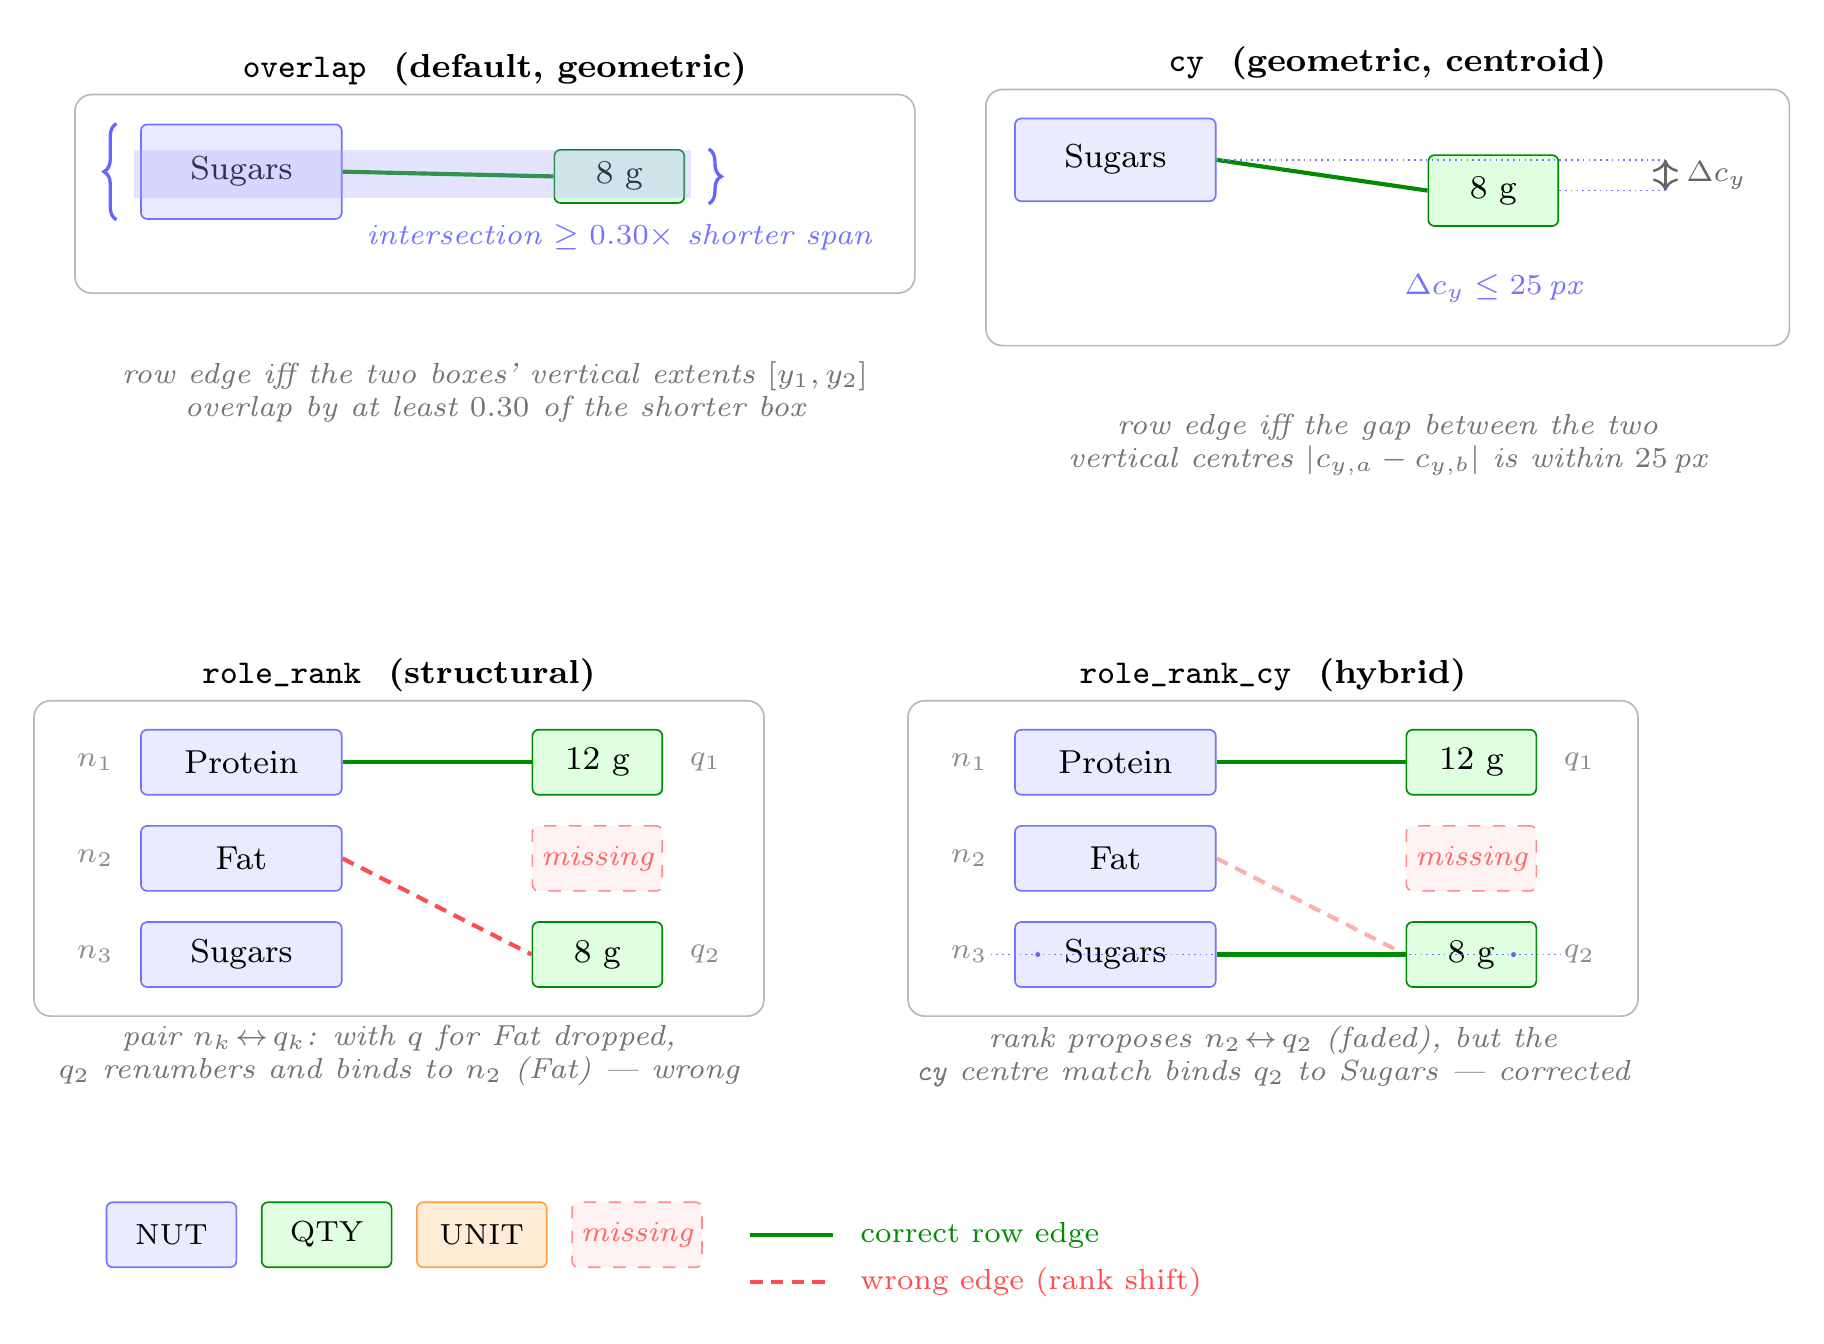
\includegraphics[width=\linewidth]{row_modes.png}%
  }{%
    \fbox{\parbox[c][55mm][c]{0.92\linewidth}{\centering\itshape
      Row-mode comparison figure placeholder. Replace with
      \mcode{row_modes.png}.}}%
  }
  \caption[The four  row-compatibility edge modes]{%
    The four  row-compatibility edge edge-construction modes on the same input, where the quantity of \emph{Fat} has been dropped by OCR. The geometric modes \mcode{overlap} and vertical-centre mode link each quantity to its visually aligned nutrient and correctly leave \emph{Fat} unmatched; \mcode{overlap} decides on the intersection of the two boxes' vertical extents, while vertical-centre mode decides on the gap between their vertical centres. The structural mode  role-rank mode pairs the \(k\)-th nutrient with the \(k\)-th quantity, so the missing entry renumbers \(q_2\) and binds the \mcode{8\,g} value to \emph{Fat}. The hybrid mode  role-rank plus vertical-centre mode would propose the same incorrect rank link, but the geometric alignment overrides it and restores the correct row.}
  \label{fig:row-modes}
\end{figure}

The column relation,  column-compatibility edge, is constructed using a smaller set of modes. The default mode is \mcode{overlap}, which connects tokens when the intersection of their horizontal spans \([x_1, x_2]\) covers at least \(0.20\) of the shorter span. The horizontal-centre mode mode is a centre-based alternative that links tokens whose horizontal centres are within a fixed band of approximately \(20\) pixels. A third option,  column-identifier mode, uses the column identifiers assigned during enrichment. These modes allow the experiments to test whether shared horizontal extent, centre proximity, or induced column structure is more useful for the association task.

Context handling is also improved in graph~v2. The context-scope edge edge links a context token to relevant tokens in its scope, but it is no longer limited to nutrient nodes. It can also reach quantities and units, which is important because the context usually defines the basis of a value, not only the nutrient name. This edge also uses a lateral gate. In the default \mcode{overlap} setting, the context token and the governed token must share at least \(0.10\) of their horizontal extent. In the vertical-centre mode setting, no lateral gate is applied, and the edge is based only on vertical scope.

Graph~v2 also introduces the header-scope edge edge. This relation uses the induced column structure to connect detected headers with the tokens in the same column. It is especially useful when a label contains multiple value columns with different contexts. For example, one column may report values per 100~g, while another reports values per serving. If both headers appear at a similar vertical position, a purely vertical context rule may not separate them reliably. The column-based header relation gives the graph another way to keep these context streams distinct.

\begin{figure}[htbp]
  \centering
  \IfFileExists{calib_overlap_sweep.png}{%
    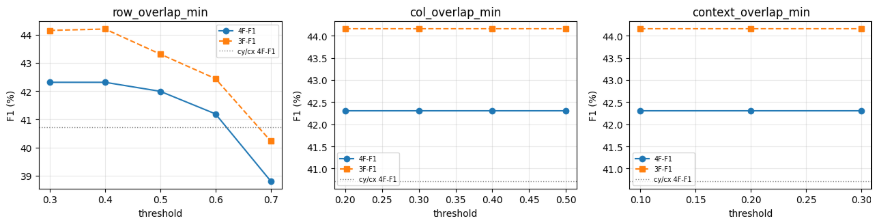
\includegraphics[width=\linewidth]{calib_overlap_sweep.png}%
  }{%
    \fbox{\parbox[c][40mm][c]{0.92\linewidth}{\centering\itshape
      Overlap-threshold sweep placeholder. Replace with
      \mcode{calib_overlap_sweep.png}.}}%
  }
  \caption[Overlap-threshold calibration for graph~v2]{%
    Coordinate-descent calibration of the three \mcode{overlap} thresholds in graph~v2, sweeping one threshold at a time while holding the other two fixed. Each panel reports 4F-F1 and 3F-F1 against the swept value; the dotted line marks the vertical-centre mode/horizontal-centre mode centroid baseline. The row threshold is the decisive axis: 4F-F1 peaks at minimum row overlap ~$=0.30$ and degrades beyond it, whereas minimum column overlap  and minimum context overlap  are flat, confirming the values \(0.20\) and \(0.10\). These operating points define the default \mcode{overlap} configuration.}
  \label{fig:overlap-sweep}
\end{figure}

\subsection{What graph v2 adds}\label{sec:graph-summary}

Overall, graph~v2 extends graph~v1 by using the enriched token representation rather than only raw bounding-box geometry. This allows the graph to use configurable row and column relations, structural attributes such as column roles and dosage streams, and more direct context links through context-scope edge and header-scope edge. In the experiments, graph~v1 is therefore kept as the simple geometry-based baseline, while graph~v2 is used to test whether the additional enrichment and context-aware edge construction improve tuple association.
% =====================================================================
% 4.6 GRAPH MATCHING AND ASSOCIATION
% =====================================================================
\section{Graph Matching and Association}\label{sec:association}

The final graph-based stage converts the semantic graph into the output tuples. At this stage, the pipeline has already identified the token roles and created typed edges between related tokens. What remains is the actual association problem: selecting the quantity that belongs to each nutrient, attaching the correct unit to that quantity, and assigning the context under which the value should be interpreted.

The association stage is deterministic and zero-shot. It does not learn parameters from the target dataset, and it does not optimise a global objective over the full table. Instead, it follows a local greedy strategy. Each nutrient node is processed in turn, and the associator searches its graph neighbourhood for plausible quantities, units, and context tokens. This design keeps the behaviour simple to inspect during error analysis, although it also means that some conflicts between competing associations are not resolved globally.

Two graph-based associators are used. The first is paired with graph~v1, the naive geometry-based constructor. The second is paired with graph~v2, the enriched geometry-aware constructor. Both associators follow the same general traversal logic, but the graph~v2 associator can use richer edge types and token attributes to handle more complex layouts.

\subsection{The shared traversal core}\label{sec:association-core}

Both graph-based associators start from a nutrient node. For each token labelled as \textsc{nutrient}, the associator searches the graph for related \textsc{quantity} nodes, mainly through row-compatible edges. Candidate quantities are ordered from left to right, which is useful in multi-column labels where values often appear in a meaningful column order.

If no suitable quantity is found through the row relation, the associator uses fallback paths through column-related and nearby edges. This helps in cases where the quantity is visually separated from the nutrient, or where a row edge was missed because of OCR segmentation or irregular spacing.

After a quantity is selected, the associator resolves the remaining fields. The unit is selected using a short fallback chain that checks fused units, same-row units, nearby units, and finally units on the nutrient row. The context is resolved after the quantity and unit, with priority given to context information close to the value side. This is important because, in multi-column tables, the context is often attached to the value column rather than to the nutrient name itself.

For each resolved association, the system emits a tuple \((n, q, u, x)\). Duplicate outputs are removed when multiple graph paths lead to the same nutrient--quantity association. However, the associator does not enforce a global one-to-one matching across the whole table. It remains a greedy local method, which keeps the process simple and inspectable but may leave some conflicts unresolved.

\subsection{Extensions in the graph v2 associator}\label{sec:association-v2}

The graph~v2 associator keeps the same general traversal idea, but adds several mechanisms for more complex layouts. The first addition is per-quantity context. Since graph~v2 allows context-scope edge and header-scope edge edges to reach value-bearing tokens, different quantities on the same nutrient row can receive different contexts. This is useful when one column reports values per 100~g, while another reports values per serving or per daily dose.

The second addition is dosage-stream matching. When the enrichment stage separates value columns into different dosage streams, graph~v2 can associate the same nutrient with values from each stream separately. This allows the system to output multiple tuples for the same nutrient when the label reports it under different contexts.

The third addition is unit refinement. Instead of taking the first suitable unit found by the fallback chain, graph~v2 prefers the unit closest to the right of the quantity on the same tight line. This reduces errors in dense tables where a loose row relation may include a unit from a neighbouring row.

The fourth addition is energy-aware filtering. Energy rows are treated as a special case because they are usually reported in \mcode{kJ} or \mcode{kcal}. When the nutrient is an energy term, such as \mcode{Energie}, \mcode{Brennwert}, or \mcode{energy}, the associator prefers quantities with energy units and avoids capturing nearby gram or milligram values.

These additions make graph~v2 better suited for multi-column and context-rich supplement labels. Graph~v1 remains useful as a simpler baseline, while graph~v2 tests the value of the enriched graph representation during association.

\subsection{Fallback extraction for non-tabular layouts}\label{sec:association-fallback}

A regex-based fallback is included for cases where OCR returns paragraph-like text rather than separated table cells. It is activated only when the graph stage produces very few tuples compared with the number of detected quantities. The fallback scans the fused text for multilingual nutrient names followed by quantity--unit groups and emits the corresponding tuples directly.

This fallback improves recall on labels where the table structure is not available in the OCR output. However, it remains limited by OCR quality and does not replace the graph-based association used for table-like layouts. Remaining errors from these cases are discussed later in Chapter~\ref{chap:experiments}.
% =====================================================================
% 4.7 VISION--LANGUAGE ASSOCIATION FROM AN INJECTED TOKEN TABLE
% =====================================================================
\section{Vision--Language Association from an Injected Token Table}\label{sec:vlm-assoc}

The third association variant replaces the graph traversal step with a vision--language model. The earlier parts of the pipeline are kept unchanged: the label image is still processed by OCR, the detected tokens are corrected, and semantic roles are assigned. The difference appears only at the final association stage. Instead of using graph edges to form tuples, the corrected token table is passed to the model, and the model is asked to decide how the tokens should be grouped into nutrient tuples.

This variant is included mainly as a point of comparison rather than as the primary approach of the thesis. The idea is to see whether a general-purpose vision--language model can carry out the binding step when it is given exactly the same OCR-derived information as the graph matcher. One important limitation, however, is that the model behaves largely as a black box. It can produce the final nutrient tuples, but it does not explain why a specific nutrient was paired with a particular quantity. In contrast, the graph-based approaches provide a much clearer and more interpretable association process, since the connections can be traced through explicit graph paths and edges.

\subsection{The injected prompt}\label{sec:vlm-assoc-prompt}

The model receives the original label image together with an injected token table. Each row in the table represents one surviving token and contains its index, text, semantic role, and pixel coordinates. Tokens labelled as \textsc{nrv} or \textsc{noise} are removed before injection, so the table focuses only on the four roles needed for tuple construction: nutrient, quantity, unit, and context. The structural attributes produced by the enrichment stage are not included by default.

The prompt treats the problem as one of association rather than text recognition. The model is explicitly told to rely on the injected token table for the textual content and to use the image only for visual cues such as alignment, proximity, and table headers. This setup was chosen to keep the comparison with the graph-based approaches fair, since those methods also work solely with the OCR tokens produced in earlier stages. For this variant, Gemma 3 4B~\cite{gemma3} is used through a locally hosted OpenAI-compatible endpoint. The generation temperature is kept low to encourage more consistent outputs.

\subsection{Output and normalisation}\label{sec:vlm-assoc-output}

The model is instructed to return a bare JSON array. Each object in the array contains four fields: \texttt{nutrient}, \texttt{quantity}, \texttt{unit}, and \texttt{context}. The prompt also requires the model to use only information from the injected token table and to avoid creating associations that are not supported by the provided tokens. If the response is cut off because of the token limit, the parser attempts to recover any complete JSON objects from the partial output.

Before evaluation, the predicted tuples are normalised. Quantity and unit strings are lightly cleaned, and context values are mapped to canonical forms such as \mcode{per_100g} and \mcode{per_serving}. Nutrient names are normalised using the same C15 mapping used elsewhere in the pipeline.

The placement of C15 is important in this variant. In the graph-based paths, C15 is applied before association, so the matcher works directly with canonical nutrient names. In the vision--language path, the token table is injected before C15 is applied. This choice is intentional. The model also sees the original image, where the text still appears in its original surface form, for example \texttt{Eiwei{\ss}} or \texttt{davon Zucker}. If the injected table had already replaced these forms with \texttt{Protein} or \texttt{Sugars}, the token text would no longer match what is visible in the image. For this reason, the VLM first receives the corrected surface forms, and C15 is applied only after the model has produced its tuples. This keeps the VLM input consistent with the image while still evaluating all variants using the same canonical vocabulary.      % NOTE: uncomment when written

% ----------------------------------------------------------------------
% Chapter 5 — Dataset and Evaluation
% ----------------------------------------------------------------------
% =====================================================================
%  CHAPTER 5 — DATASET AND EVALUATION
%  Zero-Shot Nutrient and Quantity Association using
%  OCR-Guided Semantic Graph Matching
%  Moustafa Hamada | THD + USB
%
%  Build: scrbook, XeLaTeX + BibTeX. Citations: \cite{}. Cross-refs: \S\ref{}.
%  Packages used here (graphicx, booktabs, placeins) are already loaded
%  for Chapter 4 -- nothing new to add to the preamble.
%
%  LABELS USED IN THIS FILE (align to your actual labels if they differ):
%    chap:evaluation
%    sec:corpus, sec:schema (+ -tuple, -annotation, -normalisation),
%    sec:fields (+ -nutrient, -quantity, -unit, -context)
%    chap:methodology (Ch4), chap:experiments (Ch6)
%    fig:tuples-per-image, fig:nutrient-top15, fig:unit-distribution,
%    fig:context-structure, tab:density-bands, tab:schema, tab:quantity-formats
%
%  FIGURE ASSETS (place next to thesis.tex, as for the Ch4 figures; each is
%  guarded by \IfFileExists so the chapter compiles before they are present):
%    tuples_per_image_hist.png, nutrient_top15.png,
%    unit_distribution.png, context_structure.png
% =====================================================================

\chapter{Dataset and Evaluation}\label{chap:evaluation}

This chapter describes the data used to evaluate the pipeline of
Chapter~\ref{chap:methodology}, and how the pipeline is scored. It has two
parts. The first part describes the corpus: its size, the content of each
field, and its layout. The second part defines the evaluation metric and
the tuple-matching rules used in Chapter~\ref{chap:experiments}.

\section{Corpus Overview}\label{sec:corpus}

The corpus has $57$ images of nutrition labels from food and supplement
products. Some were provided by the thesis supervisor; the rest are
photographs of similar labels taken by the author in shops. Each image was
annotated as a set of tuples, following the schema in \S\ref{sec:schema},
giving $866$ tuples in total. Nothing is held out for training: the work is
zero-shot, so all $57$ images are used only for evaluation.

The number of tuples per image varies widely. The mean is $15.2$, the
median is $16$, and the standard deviation is $9.9$; the smallest image has
one tuple and the largest has $48$, with quartiles at $8$ and $18$.
Figure~\ref{fig:tuples-per-image} shows the spread. The corpus mixes two
kinds of label: short single-purpose lists, and large tables with many
nutrients and several columns.

\begin{figure}[tb]
  \centering
  \IfFileExists{tuples_per_image_hist.png}{%
    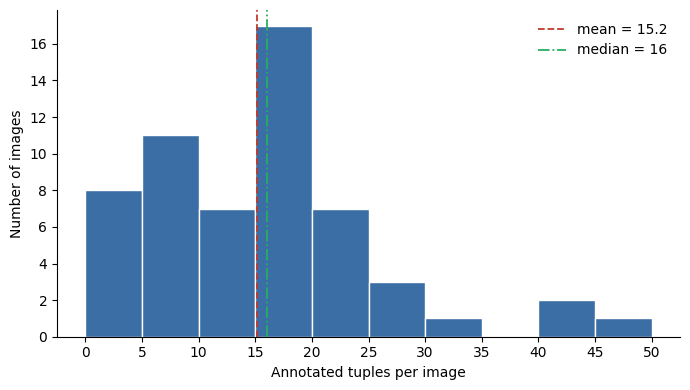
\includegraphics[width=0.8\linewidth]{tuples_per_image_hist.png}%
  }{%
    \fbox{\parbox[c][0.34\textheight][c]{0.8\linewidth}{\centering\itshape
      Tuples-per-image histogram --- placeholder. Replace with the provided
      plot \texttt{tuples\_per\_image\_hist.png} (number of tuples per image
      across the 57-image corpus).}}%
  }
  \caption[Tuples per image]{%
    Number of tuples per image, across the $57$ images. The mean is $15.2$
    and the median is $16$. Most images are small; a few dense tables form a
    long tail.}
  \label{fig:tuples-per-image}
\end{figure}

The images split into three groups by tuple count: \emph{sparse}
($1$--$9$), \emph{medium} ($10$--$20$), and \emph{dense} ($21$ or more).
Table~\ref{tab:density-bands} gives the split. Most images are medium
($50.9\%$ of images, $54.5\%$ of tuples). The outer groups are uneven:
sparse images are a third of the images ($33.3\%$) but only $12.2\%$ of the
tuples, and dense images are the opposite ($15.8\%$ of images, $33.3\%$ of
tuples).

\begin{table}[tb]
  \centering
  \caption[Image-density bands]{%
    Images grouped by tuple count. Dense images are $15.8\%$ of the images
    but hold a third of the tuples.}
  \label{tab:density-bands}
  \begin{tabular}{lrrrr}
    \toprule
    Band              & Images & \% Images & Tuples & \% Tuples \\
    \midrule
    Sparse (1--9)     & 19 & 33.3  & 106 & 12.2  \\
    Medium (10--20)   & 29 & 50.9  & 472 & 54.5  \\
    Dense ($\geq 21$) &  9 & 15.8  & 288 & 33.3  \\
    \midrule
    Total             & 57 & 100.0 & 866 & 100.0 \\
    \bottomrule
  \end{tabular}
\end{table}

This matters for scoring. The metric counts every tuple equally across the
corpus, so images with more tuples affect the score more, and the dense
images carry most of the weight. They are also the hardest, with many
nutrients, repeated columns, and sometimes poor OCR. One, \texttt{15.PNG},
has the only three-column layout in the corpus and a large OCR failure; it
returns later and in Chapter~\ref{chap:experiments}.

\FloatBarrier

\section{Annotation Schema and Protocol}\label{sec:schema}

This section defines a tuple and explains how the tuples were made: first
the schema, then the two-pass annotation, then the step that normalises the
nutrient names.

\subsection{The annotation schema}\label{sec:schema-tuple}

Each tuple is a row of seven fields, listed with an example in
Table~\ref{tab:schema}. One field, \texttt{image\_id}, names the source
image. Four fields are the extraction target and the tuple scored by the
metric (the four-field target of Chapter~\ref{chap:methodology}):
\texttt{nutrient} is the nutrient name, \texttt{quantity} is a number,
\texttt{unit} is the unit, and \texttt{context} is the basis the value is
given under (\texttt{per\_100g}, \texttt{per\_serving},
\texttt{per\_daily\_dose}, or \texttt{per\_100ml}).

Two fields are auxiliary. \texttt{nrv\_percent} is the reference-value
percentage, as a plain number. \texttt{serving\_size} is the serving or
dose, as free text; when a tuple has one, it is added to the
\texttt{context} value before scoring (for example,
\texttt{per\_serving (Pro Stick)}). Both fields are often empty, for reasons
given later in this chapter.

\begin{table}[tb]
  \centering
  \caption[The annotation schema]{%
    The seven fields, with an example row from image \texttt{106.PNG}. The
    four middle fields are the scored tuple. \texttt{serving\_size}, when
    present, is added to \texttt{context} before scoring.}
  \label{tab:schema}
  \begin{tabular}{lll}
    \toprule
    Field & Content & Example \\
    \midrule
    \texttt{image\_id}     & source image                    & \texttt{106.PNG}      \\
    \texttt{nutrient}      & nutrient name                   & Magnesium             \\
    \texttt{quantity}      & number only                     & 250                   \\
    \texttt{unit}          & unit                            & mg                    \\
    \texttt{context}       & reference basis                 & \texttt{per\_serving} \\
    \addlinespace
    \texttt{nrv\_percent}  & reference-value \%, number only & 67                    \\
    \texttt{serving\_size} & serving / dose, free text       & Pro Stick             \\
    \bottomrule
  \end{tabular}
\end{table}

Two points about the schema matter later. First, the quantity and the unit
are separate fields, and the quantity is only a number, so the unit can
change without changing the value. Second, nutrient names are kept in the
language printed on the label; they are mapped to one common form in a later
step (\S\ref{sec:schema-normalisation}), which changes only the nutrient
field.

\subsection{Two-cycle annotation}\label{sec:schema-annotation}

The tuples were made in two passes. In the first pass, a large
vision--language model (Gemini~3) read each image and wrote out its tuples
in the schema above. It was told to copy only visible text, invent nothing,
and keep nutrient names in their original language. Each quantity was a
number with the unit in a separate field. Context headers were mapped to
the fixed forms, breakdown entries such as single magnesium salts became
separate rows, qualifiers such as ``(gesamt)'' were kept, the percent sign
was dropped from the NRV field, and a field was left empty when the label
gave no value. Rows were not merged, so an energy line in both kJ and kcal
became two rows.

The second pass was manual. The author checked the model's output against
each image, corrected misreadings, added missing rows, and removed wrong
ones. This checked output is the gold standard; the first pass only saved
manual typing.

One of the baselines in Chapter~\ref{chap:experiments} is also a
vision--language model, so three facts are worth noting. The labels are
defined by the human pass, not the model: every row was checked by hand.
The model used for annotation (Gemini~3) is not the baseline model (the
smaller Gemma~3~4B). And the pipeline does not use the annotations at all.

\subsection{Nutrient-name normalisation}\label{sec:schema-normalisation}

The labels print the same nutrient in many forms: \texttt{Eiwei{\ss}},
\texttt{EIWEISS}, and \texttt{Protein} all mean protein. A final step maps
these to one common name, so a predicted name and a gold name can be
compared as strings. It changes only the nutrient field.

The mapping has three tiers. A name is first looked up in a dictionary of
exact forms. If it is not found, it is split on the separators labels use
for two languages (``Fett\,/\,fat''), and the first part is matched against
a set of patterns. A name that matches neither is kept as it is.

This has two effects, both used in the next section. First, common
nutrients become one English name (\texttt{Eiwei{\ss}} to \texttt{Protein},
``davon Zucker'' to \texttt{Sugars}), while rare names that appear once or
twice --- specific magnesium salts, plant extracts, probiotic strains ---
keep their German or Latin form. So the names are mixed: English for common
nutrients, German or Latin for rare ones. Second, the step flattens the
``of which'' rows, so a sub-nutrient such as ``davon Zucker'' is stored as
its own nutrient (\texttt{Sugars}) rather than under the one above it. After
this step the corpus has $62$ different nutrient names.

Two final points. The dictionary keeps some names apart even when they mean
the same thing: \texttt{Colecalciferol} and \texttt{Vitamin~D3} stay
separate and are counted as two. And the pipeline applies the same mapping
to its own output (rule~C15 in Chapter~\ref{chap:methodology}), so gold and
predicted names use the same vocabulary when compared.

\FloatBarrier

\section{The Four Fields}\label{sec:fields}

This section looks at the four scored fields one by one: nutrient,
quantity, unit, and context. Each has a pattern that makes it hard to read
off the label, and the context field explains why the pipeline builds a
graph.

\subsection{Nutrient names}\label{sec:fields-nutrient}

The corpus has $62$ different nutrient names, used very unevenly. The top
five cover $447$ tuples ($51.6\%$), the top ten cover $644$ ($74.4\%$), and
the top fifteen cover $713$ ($82.3\%$). Figure~\ref{fig:nutrient-top15}
shows the fifteen most common. Fifteen names ($24.2\%$ of the vocabulary)
appear only once.

\texttt{Energy} is the most common, at $152$ tuples, about twice the next.
This is because most labels print energy in both kilojoules and
kilocalories, and each is a separate tuple; counted as one nutrient, energy
would be about $76$, like fat, carbohydrate, and protein.

\begin{figure}[tb]
  \centering
  \IfFileExists{nutrient_top15.png}{%
    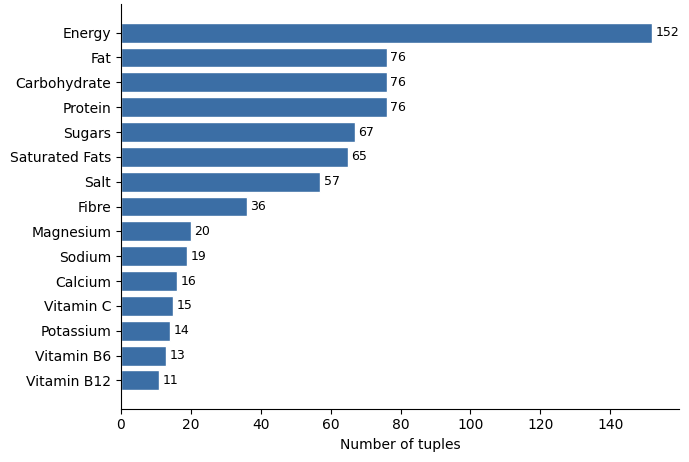
\includegraphics[width=0.85\linewidth]{nutrient_top15.png}%
  }{%
    \fbox{\parbox[c][0.34\textheight][c]{0.85\linewidth}{\centering\itshape
      Top-nutrient figure --- placeholder. Replace with the provided plot
      \texttt{nutrient\_top15.png} (the fifteen most common nutrient names by
      tuple count).}}%
  }
  \caption[Most common nutrient names]{%
    The fifteen most common nutrient names, by tuple count. \texttt{Energy}
    is highest because most labels state it twice, in kJ and kcal. The corpus
    has $62$ names in total, $15$ of which appear only once.}
  \label{fig:nutrient-top15}
\end{figure}

\subsection{Quantities}\label{sec:fields-quantity}

Almost all quantities are plain numbers: of the $866$ values, $846$ are
plain numbers, $18$ are bounds such as \texttt{<0.1}, and $2$ are in
scientific notation (Table~\ref{tab:quantity-formats}). The bounds are trace
amounts, mostly for salt or sodium. The two scientific-notation values are
bacteria counts ($3.6\times10^{8}$) on two probiotic rows.

The values cover a very wide range. The plain values run from $0.02$ to
$10\,000$, about $5.7$ orders of magnitude; with the two bacteria counts,
the range grows to about $10$ orders of magnitude. About one value in ten is
zero ($86$ of $866$), from labels stating zero sugar, fat, or salt, and none
are negative.

\begin{table}[tb]
  \centering
  \caption[Quantity formats]{%
    The three quantity formats. Almost all values are plain numbers; the
    rest are trace bounds or bacteria counts.}
  \label{tab:quantity-formats}
  \begin{tabular}{lrl}
    \toprule
    Format               & Count & Example \\
    \midrule
    Plain number         & 846 & $250$              \\
    Bound                & 18  & \texttt{<0.1}      \\
    Scientific notation  & 2   & $3.6\times10^{8}$  \\
    \bottomrule
  \end{tabular}
\end{table}

\subsection{Units}\label{sec:fields-unit}

The corpus uses $11$ units, but five cover almost everything: grams,
milligrams, micrograms, kilocalories, and kilojoules together cover $97.5\%$
of the tuples, and grams alone cover $55.5\%$
(Figure~\ref{fig:unit-distribution}). The other six are rare and fall into
two kinds. The first is equivalence units, written as a mass unit plus a
suffix, one per vitamin: mg~$\alpha$-TE for vitamin E, mg~NE for niacin,
µg~RE for vitamin A. The second is activity and count units: I.E. for
vitamin D and KBE for the probiotic strains.

\begin{figure}[tb]
  \centering
  \IfFileExists{unit_distribution.png}{%
    
\includegraphics[width=0.85\linewidth]{unit_distribution.png}%
  }{%
    \fbox{\parbox[c][0.34\textheight][c]{0.85\linewidth}{\centering\itshape
      Unit-distribution figure --- placeholder. Replace with the provided
      plot \texttt{unit\_distribution.png} (the 11 units by tuple count).}}%
  }
  \caption[Unit distribution]{%
    The $11$ units, by tuple count. Five units (g, mg, µg, kcal, kJ) cover
    $97.5\%$ of the tuples. The rest are equivalence units (such as
    mg~$\alpha$-TE) and count units (I.E., KBE).}
  \label{fig:unit-distribution}
\end{figure}

\subsection{Contexts}\label{sec:fields-context}

There are four context values: \texttt{per\_100g} ($44.0\%$),
\texttt{per\_serving} ($37.3\%$), \texttt{per\_daily\_dose} ($15.0\%$), and
\texttt{per\_100ml} ($3.7\%$). They split into two kinds. \texttt{per\_100g}
and \texttt{per\_100ml} are reference amounts; a label uses one or the
other, never both. \texttt{per\_serving} and \texttt{per\_daily\_dose} are
portions. A label can combine one reference amount with one or more
portions.

Most labels use more than one context. Of the $57$ images, $37$ ($64.9\%$)
have two or more contexts, and by tuples the share is higher: $707$ of $866$
($81.6\%$) come from these images. The most common layout is
\texttt{per\_100g} with \texttt{per\_serving}, in $27$ images
(Figure~\ref{fig:context-structure}).

This is why the pipeline needs more than a left-to-right reading. In a
multi-context label, one nutrient name has several values, one per column.
Across the corpus, $313$ of $463$ nutrient instances ($67.6\%$) have two or
more values, one per context. The name appears once but must link to two or
three different values, and the only thing separating them is which column
they sit in. A line-by-line reader cannot tell them apart; it has to use the
column positions, which is what the graph in Chapter~\ref{chap:methodology}
encodes. \texttt{15.PNG} is the hardest case, with three contexts at once,
so each nutrient links to three values.

\begin{figure}[tb]
  \centering
  \IfFileExists{context_structure.png}{%
    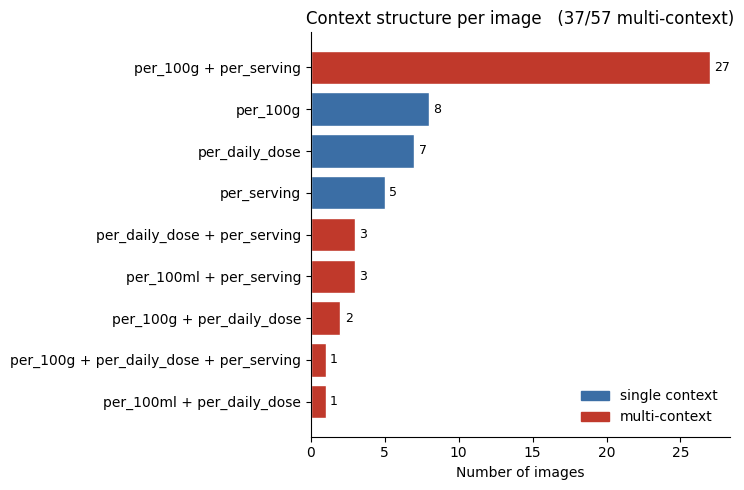
\includegraphics[width=0.85\linewidth]{context_structure.png}%
  }{%
    \fbox{\parbox[c][0.34\textheight][c]{0.85\linewidth}{\centering\itshape
      Context-layout figure --- placeholder. Replace with the provided plot
      \texttt{context\_structure.png} (context layouts across the 57
      images).}}%
  }
  \caption[Context layouts]{%
    Context layouts across the $57$ images. $37$ images ($64.9\%$) use more
    than one context. The most common layout is \texttt{per\_100g} with
    \texttt{per\_serving}.}
  \label{fig:context-structure}
\end{figure}

\FloatBarrier

 
\section{Field Completeness}\label{sec:completeness}
 
The four scored fields are almost always present. Nutrient, quantity, and
context are filled in every tuple; unit is missing in only one (an energy
value printed with no unit). So $865$ of $866$ tuples ($99.9\%$) have all
four scored fields, and the four-field tuple is well-posed for almost every
row. Figure~\ref{fig:completeness} shows the rates.
 
The two extra fields are often empty: \texttt{nrv\_percent} is filled in
$20.2\%$ of tuples and \texttt{serving\_size} in $57.6\%$. Both gaps are
structural, not missing work. \texttt{nrv\_percent} is mostly a
micronutrient field: vitamins and minerals carry a reference-value
percentage, while most macronutrient rows do not print one, so the field is
blank there because the label has no value. \texttt{serving\_size} follows
the context. It is almost always present on portion contexts
(\texttt{per\_serving}, \texttt{per\_daily\_dose}) and almost never on
reference contexts (\texttt{per\_100g}, \texttt{per\_100ml}), because a
serving size only makes sense for a portion. It is a property of the panel,
not of each row, and when present it is folded into the context value, as
\S\ref{sec:schema-tuple} describes.
 
\begin{figure}[tb]
  \centering
  \IfFileExists{field_completeness.png}{%
    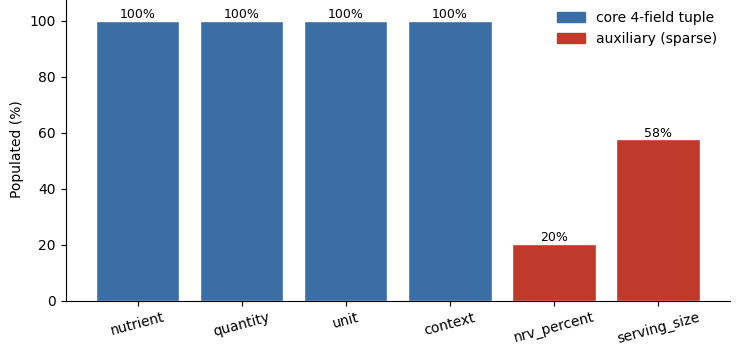
\includegraphics[width=0.8\linewidth]{field_completeness.png}%
  }{%
    \fbox{\parbox[c][0.34\textheight][c]{0.8\linewidth}{\centering\itshape
      Field-completeness figure --- placeholder. Replace with the provided
      plot \texttt{field\_completeness.png} (share of tuples with each field
      filled).}}%
  }
  \caption[Field completeness]{%
    Share of tuples with each field filled. The four scored fields are
    near-complete; \texttt{nrv\_percent} and \texttt{serving\_size} are
    sparse for structural reasons.}
  \label{fig:completeness}
\end{figure}
 
\FloatBarrier
  

% =====================================================================
%  Insert immediately BEFORE  \section{Evaluation}\label{sec:evaluation}
%  (after the \FloatBarrier that closes "Field Completeness").
%  booktabs + graphicx only (already loaded). No new figure asset.
% =====================================================================

\section{The Reduced Test Set}\label{sec:testset}

All of the labels described so far belong to the corpus, and the experiments in
Chapter~\ref{chap:experiments} are run across it. Two of them, however, are not
tables. They lack the row-and-column layout the method needs in order to pair a
nutrient with its values, which places them outside what the pipeline is built
to read. Because both were part of that data, their effect is shown directly:
the runs are scored a second time with the two labels removed, and the figures
for the full corpus and for the reduced set appear side by side.

The two labels are \texttt{15.PNG} and \texttt{67.jpeg}. Between them they hold
$46$ tuples, and the split is very uneven: $42$ come from \texttt{15.PNG}, one of
the largest labels in the whole corpus, and only $4$ from \texttt{67.jpeg}.
Taking both out leaves $55$ images and $820$ tuples, so nearly all of the
reduction traces to one dense label rather than to the pair together.

In shape, the reduced set differs only slightly from the full one.
Table~\ref{tab:testset} sets the two beside each other. The typical image is
unchanged in size: the median holds at $16$ tuples, and the mean falls just a
little, from $15.2$ to $14.9$. Contexts and units keep almost the same balance
as before, and the vocabulary loses a single name, from $62$ down to $61$,
because \texttt{Colecalciferol} was printed on a removed label and nowhere else.
Across the four scored fields the reduced set stays near-complete, with every one
of the $820$ tuples carrying a nutrient, a quantity and a context, and only one
missing its unit.

\begin{table}[tb]
  \centering
  \caption[Full corpus versus reduced test set]{%
    The full corpus and the reduced set, the latter with the two non-tabular
    labels removed. Chapter~\ref{chap:experiments} reports scores on both.
    Percentages are shares of tuples within each set.}
  \label{tab:testset}
  \begin{tabular}{lrr}
    \toprule
                              & Full corpus & Reduced set \\
    \midrule
    Images                    & 57   & 55   \\
    Tuples                    & 866  & 820  \\
    Distinct nutrients        & 62   & 61   \\
    Tuples per image (mean)   & 15.2 & 14.9 \\
    Tuples per image (median) & 16   & 16   \\
    \addlinespace
    \texttt{nutrient} filled  & 866  & 820  \\
    \texttt{quantity} filled  & 866  & 820  \\
    \texttt{unit} filled      & 865  & 819  \\
    \texttt{context} filled   & 866  & 820  \\
    \addlinespace
    \texttt{per\_100g}        & 44.0\% & 44.8\% \\
    \texttt{per\_serving}     & 37.3\% & 37.4\% \\
    \texttt{per\_daily\_dose} & 15.0\% & 13.9\% \\
    \texttt{per\_100ml}       & 3.7\%  & 3.9\%  \\
    \bottomrule
  \end{tabular}
\end{table}

One difference deserves a note, as it links back to the earlier account of
context. Of all the annotated labels, \texttt{15.PNG} alone recorded three
contexts at once. With it gone, nothing in the reduced set holds more than two,
so a nutrient name maps to two values at most rather than three. None of this
weakens the case for a graph. About two nutrient instances in three ($298$ of
$448$, or $66.5\%$) still fall under more than one context, and what separates
those values is only the column they occupy. That one label had simply shown the
pattern in its most extreme form.

\FloatBarrier



\section{Evaluation}\label{sec:evaluation}
 
The pipeline is scored by comparing its output tuples against the gold
tuples. This section defines when a tuple counts as correct, and how
predicted tuples are matched to gold tuples to compute the score.
 
\subsection{What counts as a correct tuple}\label{sec:metric}
 
A predicted tuple is correct when it matches a gold tuple in all four
fields. Each field is compared up to normalisation, so that surface
differences do not count as errors:
\begin{itemize}
  \item the \texttt{nutrient} is matched by name, allowing for differences in
        case and in German or English spelling;
  \item the \texttt{quantity} is matched by its numeric value;
  \item the \texttt{unit} is matched after treating equivalent unit names as
        the same (for example µg and mcg), while keeping kJ and kcal
        distinct;
  \item the \texttt{context} is matched as its canonical basis
        (\texttt{per\_100g}, \texttt{per\_serving}, \texttt{per\_daily\_dose},
        \texttt{per\_100ml}).
\end{itemize}
 
A tuple that matches on all four fields is a four-field (4F) match. A tuple
that matches on nutrient, quantity, and unit, ignoring context, is a
three-field (3F) match. The 4F match is the primary metric of this work; the
3F match is reported alongside it to show how much the context field costs.
 
\subsection{Matching predictions to gold}\label{sec:protocol}
 
The evaluator is deterministic: it applies the fixed rules above in a single
pass, with no model in the loop. It works per image, and the counts are then
pooled over the corpus.
 
For each image, the predicted tuples are matched to the gold tuples one to
one. Matching is greedy: the predicted tuple whose nutrient name is closest
to a gold name is paired first, with quantity and unit breaking ties, and
each gold tuple and each predicted tuple is used at most once. Each matched
pair is then scored field by field. A gold tuple with no matching prediction
is a miss, and a predicted tuple with no matching gold is a false alarm.
 
\subsection{Field-level and tuple-level scores}\label{sec:scores}
 
The pipeline is scored at two levels.
 
\paragraph{Field level.} Each field is checked on its own, over the matched
pairs. The quantity accuracy is the share of matched tuples with the right
quantity; unit and context accuracy are the same. These rates show which
field is the weak point, but they only cover tuples that were matched in the
first place.
 
\paragraph{Tuple level.} The whole tuple is judged together and counts as
correct only if all four fields match (or three, for 3F). This is the
strict, headline measure, and it uses three numbers:
\begin{itemize}
  \item \emph{precision} is the share of predicted tuples that are correct;
        it drops when the pipeline outputs wrong or extra tuples;
  \item \emph{recall} is the share of gold tuples that are found; it drops
        when the pipeline misses tuples;
  \item \emph{F1} is the harmonic mean of precision and recall --- one number
        that is high only when both are high.
\end{itemize}
The tuple-level scores are pooled over all $866$ gold tuples, so every tuple
counts equally (\S\ref{sec:corpus}). The 4F F1 is the primary metric of this
work, with 3F F1 reported alongside.
 
\FloatBarrier



% ----------------------------------------------------------------------
% Chapter 6 — Experiments and Results
% ----------------------------------------------------------------------

\chapter{Experiments and Results}\label{chap:experiments}

This chapter evaluates the pipeline described in Chapter~\ref{chap:methodology}. Instead of presenting the results as a disconnected list of scores, the chapter is organised around five experimental questions. Each question corresponds to one main design choice in the pipeline:

\begin{enumerate}
\item Which OCR engine reads nutrition labels most accurately?
(Section~\ref{sec:exp-ocr})
\item Which semantic classifier detects nutrient entities most reliably?
(Section~\ref{sec:exp-classifier})
\item Which association engine builds better tuples, graph~v1 or
graph~v2? (Section~\ref{sec:exp-assoc})
\item If a vision--language model is used only at the association step,
does it perform better than the graph-based association method, and
how does it compare with a fully end-to-end vision--language model
that maps the image directly to tuples?
(Section~\ref{sec:exp-vlm})
\item Which edge-creation mode performs best inside graph~v2?
(Section~\ref{sec:exp-edge})
\end{enumerate}

The first two questions focus on the OCR and semantic classification stages. The last three questions all relate to the association stage, but they examine it from different perspectives: the choice of graph engine, the possible use of a vision--language model for association, and the effect of the edge-creation mode inside graph~v2.

To answer these questions, 14 pipeline configurations were evaluated. In each experiment, the pipeline is kept unchanged except for the component being tested. This allows changes in performance to be linked to the stage under investigation, rather than to unrelated changes elsewhere in the system. Figure~\ref{fig:ablation-tree} presents the full experimental design as a single ablation tree and serves as the map for the rest of this chapter. Each leaf represents one experiment. The path leading to that leaf shows the OCR engine, classifier, association engine, and edge mode used in that configuration, while the value at the leaf reports the four-field tuple F1 score (4F-F1).

The dataset, annotation schema, evaluation metrics, and tuple-matching procedure were already defined in Chapter~\ref{chap:evaluation}, so they are not repeated here. Unless stated otherwise, the term ``best'' refers to the highest 4F-F1 score. However, not every experimental question can be answered by this score alone. For example, the OCR comparison also considers per-field accuracy, the classifier comparison reports nutrient-field metrics, and the graph and vision--language experiments additionally examine performance on single-context and multi-context images. When precision or recall changes the interpretation of a ranking, the corresponding section reports these values separately.
\begin{figure}[p]
  \centering
  \makebox[\textwidth][c]{%
    \includegraphics[width=1.2\textwidth,height=1.1\textheight,keepaspectratio]%
      {ablation_tree_portrait.png}%
  }
  \caption[Ablation results tree]{%
Summary tree of the 14 ablation experiments. Each path shows the OCR
engine, classifier, association method, and, for graph~v2, the
edge-creation mode. Leaves report 4F-F1. Border styles indicate
interpretability tiers, colours distinguish OCR engines, amber marks
graph~v2 edge-mode variants, the filled diamond marks the best edge
mode, and the star marks the best fully interpretable pipeline.}

  \label{fig:ablation-tree}
\end{figure}
% =====================================================================
%  6.1  EXPERIMENTAL SETUP
% =====================================================================
\section{Experimental Setup}\label{sec:exp-setup}

This section records the configuration held fixed across the experiments
and lists the runs. The dataset, the annotation schema, the four-field
(4F) and three-field (3F) tuple metrics, and the tuple-matching procedure
used for scoring are defined in Chapter~\ref{chap:evaluation} and are
reused here without restatement. Every result in this chapter is produced
by the same evaluator on the test set of 57 labelled images and 866 gold
tuples, so all scores are directly comparable.

The fixed backbone is as follows. PaddleOCR PP-OCRv5 is the OCR engine for
every run except the EasyOCR baseline used to settle the OCR axis
(Section~\ref{sec:exp-ocr}). When graph~v2 is the association engine it
uses the \mcode{overlap} edge mode, with default row, column, and context
overlap thresholds of 0.30, 0.20, and 0.10. The two learned classifiers
run at fixed, calibrated operating points---GLiNER-biomed at its selected
score threshold and the BGE-M3 embedding classifier at its selected
threshold and margin---which are reported in
Section~\ref{sec:exp-classifier}. The vision--language model used at the
association step and end to end is Gemma~3~4B Instruct.

All scoring is done by the evaluator of Chapter~\ref{chap:evaluation}. It
is fully reproducible, returning the same scores on every run, so the
comparison across runs is exact. The primary metric is the four-field
tuple F1 (4F-F1), the share of gold tuples whose nutrient, quantity,
unit, and context are all correct; the three-field tuple F1 (3F-F1),
which drops the context field, is reported alongside it where it adds
information.

Table~\ref{tab:exp-registry} lists the runs used in this chapter. Each run
is named by the label used throughout, and is defined by its OCR engine,
classifier, association engine, and (for graph~v2) edge mode; the headline
column is its four-field tuple F1. The four additional graph~v2
edge-mode variants used only in Section~\ref{sec:exp-edge} are introduced
there and are not listed here.

\begin{table}[htbp]
  \centering
  \caption[Experiment registry]{The runs used in this chapter. Each run is
    identified by the label used throughout and is defined by its OCR
    engine, semantic classifier, association engine, and graph~v2 edge
    mode. The run \mbox{E2-A} is the PaddleOCR rule-based reference,
    also referred to as EXP-02. Two 4F-F1 columns are given: the full test
    set (866 tuples, 57 images) and the reduced set
    (820~tuples, 55~images) with images 15 and 67 removed, as defined in
    Chapter~\ref{chap:evaluation}. The remaining metrics appear in the
    indicated sections and are reported on the full set.}
  \label{tab:exp-registry}
  \small
  \begin{tabular}{@{}llllccc@{}}
    \toprule
     & & & & & \multicolumn{2}{c}{\textbf{4F-F1}} \\
    \cmidrule(lr){6-7}
    \textbf{ID} & \textbf{OCR} & \textbf{Classifier} & \textbf{Association} & \textbf{Edge mode} & \textbf{Full (866)} & \textbf{Reduced (820)} \\
    \midrule
    EXP-01          & EasyOCR    & Rule-based & Graph~v2       & \mcode{overlap} & 0.1773 & 0.1833 \\
    \addlinespace
    E2-A            & PaddleOCR  & Rule-based & Graph~v2       & \mcode{overlap} & 0.4231 & 0.4262 \\
    E2-B            & PaddleOCR  & Embedding  & Graph~v2       & \mcode{overlap} & 0.4025 & 0.4049 \\
    E2-C            & PaddleOCR  & GLiNER     & Graph~v2       & \mcode{overlap} & 0.4304 & 0.4341 \\
    \addlinespace
    E3-EMB-G1       & PaddleOCR  & Embedding  & Graph~v1       & ---             & 0.2325 & 0.2392 \\
    E3-GLiNER-G1    & PaddleOCR  & GLiNER     & Graph~v1       & ---             & 0.2523 & 0.2599 \\
    \addlinespace
    A\_VLM          & PaddleOCR  & Rule-based & VLM assoc.\    & ---             & 0.4819 & 0.4944 \\
    E3-EMB-VLM      & PaddleOCR  & Embedding  & VLM assoc.\    & ---             & 0.4945 & 0.5092 \\
    E3-GLiNER-VLM   & PaddleOCR  & GLiNER     & VLM assoc.\    & ---             & 0.4446 & 0.4555 \\
    \addlinespace
    E4              & ---        & ---        & End-to-end VLM & ---             & 0.3597 & 0.3704 \\
    \bottomrule
  \end{tabular}
\end{table}

The two columns track together. Removing images 15 and 67 raises every run
slightly---between 0.002 and 0.015 in four-field F1---and changes no
position in the ranking: E3-EMB-VLM stays highest overall, E2-C stays the
best fully interpretable run, and EXP-01 stays lowest. The gains are small
because both removed images were among the weakest in the set. The rest of
this chapter reports on the full set of 866 tuples; the reduced column is
given here so the two test sets can be compared directly.

% =====================================================================
%  6.2  OCR AXIS
% =====================================================================
\section{OCR Engine}\label{sec:exp-ocr}

The first question is which OCR engine reads the labels best. Two engines
are compared: EasyOCR and PaddleOCR PP-OCRv5. Everything after the OCR
stage is held fixed---the rule-based classifier, graph~v2 with the
\mcode{overlap} edge mode, and the same association and evaluation
steps---so any difference in the score comes from the OCR engine alone.
This axis is settled first, because OCR quality limits every later stage,
and the winning engine is then used for the rest of the chapter. The two
runs are EXP-01 (EasyOCR) and E2-A (PaddleOCR), also called EXP-02.

The OCR engine is not measured by the tuple score alone. Its real job is
to deliver tokens that the later stages can read correctly, so the first
table reports per-field accuracy: how often the nutrient, quantity, unit,
and context are correct once a nutrient has been matched.
Table~\ref{tab:ocr-fields} shows these numbers.

\begin{table}[htbp]
  \centering
  \caption[OCR axis: field-level results]{Field-level results for the two
    OCR engines, with the downstream pipeline held fixed (rule-based
    classifier, graph~v2, \mcode{overlap}). Nutrient detection is reported
    as precision, recall, and F1; the quantity, unit, and context fields
    are reported as accuracy over matched nutrients. PaddleOCR wins every
    field.}
  \label{tab:ocr-fields}
  \small
  \begin{tabular}{@{}lcccccc@{}}
    \toprule
     & \multicolumn{3}{c}{\textbf{Nutrient}} & \textbf{Quantity} & \textbf{Unit} & \textbf{Context} \\
    \cmidrule(lr){2-4}
    \textbf{OCR engine} & P & R & F1 & acc & acc & acc \\
    \midrule
    EasyOCR (EXP-01)    & 0.6667 & 0.6882 & 0.6773 & 0.4547 & 0.5168 & 0.6141 \\
    PaddleOCR (E2-A)    & 0.7227 & 0.7252 & 0.7239 & 0.7691 & 0.8121 & 0.8726 \\
    \addlinespace
    \textbf{Difference} & +0.0560 & +0.0370 & +0.0466 & +0.3144 & +0.2953 & +0.2585 \\
    \bottomrule
  \end{tabular}
\end{table}

\begin{figure}[t]
  \centering
  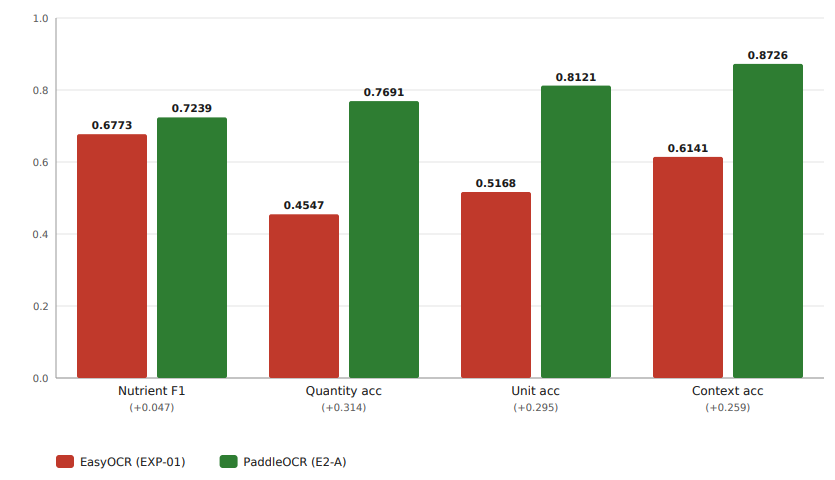
\includegraphics[width=1.2\linewidth,keepaspectratio]{ocr_fields_bars.png}
  \caption[OCR engine: per-field performance]{Per-field performance of the
    two OCR engines, with the downstream pipeline fixed (rule-based
    classifier, graph~v2, \mcode{overlap}). Nutrient is reported as F1;
    quantity, unit, and context as accuracy over matched nutrients. The two
    engines are close on nutrient detection, but PaddleOCR is far ahead on
    quantity, unit, and context---the value fields---which is where the
    full-tuple gain comes from.}
  \label{fig:ocr-fields-bars}
\end{figure}

The pattern is clear. Both engines find nutrient names about equally well:
nutrient recall rises by only about 4~points with PaddleOCR, and EasyOCR
even produces slightly more candidate tokens overall. The large gap is in
reading the values. PaddleOCR improves quantity accuracy by about
31~points, unit accuracy by about 30~points, and context accuracy by
about 26~points. In other words, EasyOCR can locate the text but often
misreads the numbers and short unit tokens, while PaddleOCR reads them
correctly. This matters because a tuple is only counted when all four
fields are right, so an error in the quantity or unit field is enough to
lose the tuple even when the nutrient name was found.

The full-tuple scores in Table~\ref{tab:ocr-tuple} follow directly from
this. The per-field gains in quantity, unit, and context combine, and the
four-field tuple F1 more than doubles, from 0.1773 to 0.4231.

\begin{table}[htbp]
  \centering
  \caption[OCR axis: full-tuple results]{Full-tuple results for the two
    OCR engines, downstream fixed. Scores are reported for the
    three-field tuple (3F, nutrient--quantity--unit) and the four-field
    tuple (4F, including context), each as precision, recall, and F1.}
  \label{tab:ocr-tuple}
  \small
  \begin{tabular}{@{}lcccccc@{}}
    \toprule
     & \multicolumn{3}{c}{\textbf{3F (n,q,u)}} & \multicolumn{3}{c}{\textbf{4F (n,q,u,x)}} \\
    \cmidrule(lr){2-4}\cmidrule(lr){5-7}
    \textbf{OCR engine} & P & R & F1 & P & R & F1 \\
    \midrule
    EasyOCR (EXP-01)    & 0.2327 & 0.2402 & 0.2364 & 0.1745 & 0.1801 & 0.1773 \\
    PaddleOCR (E2-A)    & 0.4407 & 0.4423 & 0.4415 & 0.4223 & 0.4238 & 0.4231 \\
    \bottomrule
  \end{tabular}
\end{table}

The conclusion of this axis is that PaddleOCR PP-OCRv5 is the stronger
engine, and the gain comes from reading quantities and units rather than
from finding more nutrient names. PaddleOCR is therefore fixed as the OCR
engine for all remaining experiments in this chapter.

% =====================================================================
%  6.3  CLASSIFIER AXIS
% =====================================================================
\section{Semantic Classifier}\label{sec:exp-classifier}

The second question is which semantic classifier detects nutrients best.
Three classifiers are compared: the rule-based lexicon, the BGE-M3
embedding classifier, and GLiNER-biomed. PaddleOCR is now fixed, and the
rest of the pipeline is held constant (graph~v2 with the \mcode{overlap}
edge mode), so any difference comes from the classifier. The three runs
are E2-A (rule-based), E2-B (embedding), and E2-C (GLiNER).
Figure~\ref{fig:classified-tokens} shows the embedding classifier's token
labels on two example labels, each coloured by its predicted role.

\begin{figure}[htbp]
  \centering
  \begin{minipage}[t]{0.330\textwidth}
    \centering
    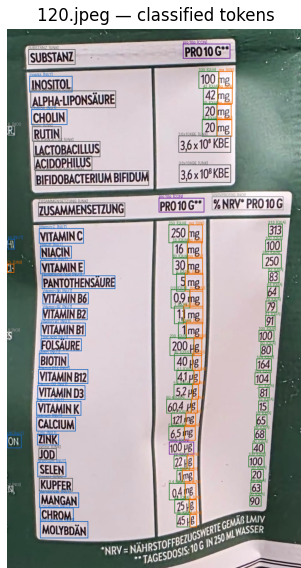
\includegraphics[width=\linewidth]{classified_tokens_120.png}\\[3pt]
    {\small (a)}
  \end{minipage}\hfill
  \begin{minipage}[t]{0.610\textwidth}
    \centering
    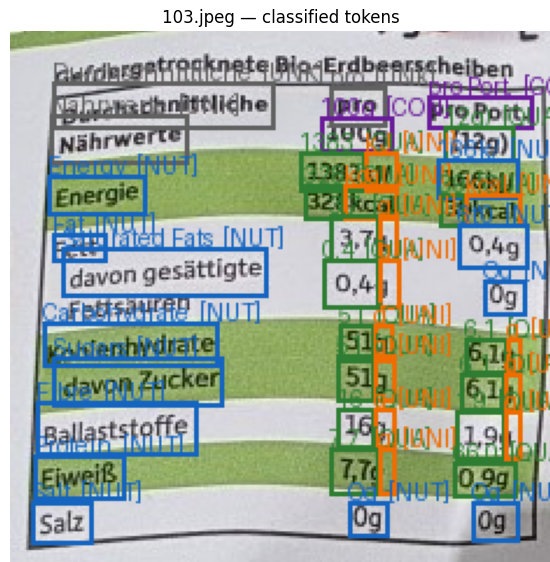
\includegraphics[width=\linewidth]{classified_tokens_103.png}\\[3pt]
    {\small (b)}
  \end{minipage}
  \caption[Classified tokens from the embedding classifier]{%
    Token classification produced by the BGE-M3 embedding classifier on two
    example labels: (a)~a dense supplement panel (120.jpeg) and (b)~a standard
    nutrition table (103.jpeg). Each detected token is boxed and coloured by its
    predicted role --- nutrient (blue), quantity (green), unit (orange), and
    context (purple). The four roles are the four scored tuple fields.}
  \label{fig:classified-tokens}
\end{figure}

One point must be made before the numbers, because it decides how this
axis is read. The three classifiers share the entire deterministic
cascade described in Section~\ref{sec:classifier-cascade}. Quantity,
unit, context, NRV, and noise are all resolved by that shared cascade and
are identical across the three runs. The only thing that changes is the
final nutrient / not-nutrient decision. The classifier axis is therefore
measured directly on the nutrient field; the quantity, unit, and context
fields are reported as well, but any movement in them is an indirect
effect of a different nutrient set changing which rows the graph builds,
not the classifier acting on those fields.

Table~\ref{tab:classifier-fields} shows this. The nutrient field is given
as precision, recall, and F1; the other three fields are given as
accuracy. The nutrient numbers move by several points across the three
classifiers, while the quantity, unit, and context accuracies stay within
about two points of each other---direct evidence that the shared cascade,
not the classifier, owns those fields.

\begin{table}[htbp]
  \centering
  \caption[Classifier axis: field-level results]{Field-level results for
    the three classifiers, with OCR fixed to PaddleOCR and the downstream
    pipeline fixed (graph~v2, \mcode{overlap}). The nutrient field is
    reported as precision, recall, and F1; quantity, unit, and context
    are reported as accuracy over matched nutrients. The nutrient field is
    the only one the classifier controls; the other three are resolved by
    the shared deterministic cascade and barely change.}
  \label{tab:classifier-fields}
  \small
  \begin{tabular}{@{}lcccccc@{}}
    \toprule
     & \multicolumn{3}{c}{\textbf{Nutrient}} & \textbf{Quantity} & \textbf{Unit} & \textbf{Context} \\
    \cmidrule(lr){2-4}
    \textbf{Classifier} & P & R & F1 & acc & acc & acc \\
    \midrule
    Rule-based (E2-A) & 0.7227 & 0.7252 & 0.7239 & 0.7691 & 0.8121 & 0.8726 \\
    Embedding (E2-B)  & 0.6580 & 0.6975 & 0.6771 & 0.7649 & 0.8311 & 0.8642 \\
    GLiNER (E2-C)     & 0.7350 & 0.6374 & 0.6827 & 0.7627 & 0.8315 & 0.8786 \\
    \bottomrule
  \end{tabular}
\end{table}

The three classifiers behave differently on the nutrient field. The
rule-based lexicon has the highest nutrient recall, 0.7252, because the
labels in this dataset are largely covered by its curated entries; its
weakness is that it is closed-vocabulary by construction. Among the two
learned classifiers, the embedding classifier has the higher recall,
0.6975 against GLiNER's 0.6374, because it accepts candidates by semantic
similarity rather than exact coverage and so recovers nutrient names that
GLiNER's threshold rejects. The cost of that recall is precision: the
embedding classifier has the lowest nutrient precision, 0.6580, so it also
admits the most non-nutrient tokens. GLiNER is the opposite---the highest
nutrient precision, 0.7350, and the lowest recall.

These thresholds were set by the token-level calibration described in
Section~\ref{sec:classifier-embedding} and
Section~\ref{sec:classifier-gliner}. The embedding classifier runs at a
cosine threshold of 0.59 with a margin of 0.04, where its token-level
nutrient F1 is about 0.87. GLiNER runs at a span threshold of 0.18, where
its token-level nutrient F1 is about 0.89, with precision 0.91 and recall
0.87. The rule-based classifier has no threshold; it accepts a candidate
when the lexicon or one of its supporting rules matches.

The full-tuple ranking in Table~\ref{tab:classifier-tuple} is the
downstream consequence of these nutrient decisions passing through the
fixed cascade and the fixed graph. GLiNER gives the best four-field F1,
0.4304, followed by the rule-based classifier at 0.4231 and the embedding
classifier at 0.4025.

\begin{table}[htbp]
  \centering
  \caption[Classifier axis: full-tuple ranking]{Full-tuple ranking of the
    three classifiers, OCR and downstream fixed. Scores are the
    three-field tuple (3F) and four-field tuple (4F), each as precision,
    recall, and F1. Rows are ordered by 4F-F1.}
  \label{tab:classifier-tuple}
  \small
  \begin{tabular}{@{}lcccccc@{}}
    \toprule
     & \multicolumn{3}{c}{\textbf{3F (n,q,u)}} & \multicolumn{3}{c}{\textbf{4F (n,q,u,x)}} \\
    \cmidrule(lr){2-4}\cmidrule(lr){5-7}
    \textbf{Classifier} & P & R & F1 & P & R & F1 \\
    \midrule
    GLiNER (E2-C)     & 0.4807 & 0.4169 & 0.4465 & 0.4634 & 0.4018 & 0.4304 \\
    Rule-based (E2-A) & 0.4407 & 0.4423 & 0.4415 & 0.4223 & 0.4238 & 0.4231 \\
    Embedding (E2-B)  & 0.4085 & 0.4330 & 0.4204 & 0.3911 & 0.4145 & 0.4025 \\
    \bottomrule
  \end{tabular}
\end{table}

The reason GLiNER wins on the tuple score even though it does not have the
best nutrient recall is precision. Its high nutrient precision means few
non-nutrient tokens enter the graph, so few false-positive tuples are
produced, and it has the highest four-field precision, 0.4634. The
embedding classifier shows the opposite effect. Its surplus nutrient
candidates are passed to the graph, which binds them into tuples without
re-checking whether they are real, so they become false-positive tuples.
This gives the embedding classifier the lowest four-field precision,
0.3911, and the lowest four-field F1, even though its nutrient recall is
higher than GLiNER's. This precision penalty is specific to the graph
association engine; Section~\ref{sec:exp-vlm} shows that it disappears when
the vision--language model handles association, which is where the
embedding classifier's recall becomes an advantage.

For the rest of the chapter, GLiNER is treated as the main zero-shot
classifier, because it gives the best interpretable tuple score without a
manually curated lexicon. The embedding classifier is kept as the second
zero-shot variant, and the rule-based classifier as a strong
closed-vocabulary reference.



% =====================================================================
%  6.4  ASSOCIATION AXIS — GRAPH V1 vs GRAPH V2
% =====================================================================
\section{Association Engine: Graph v1 versus Graph v2}\label{sec:exp-assoc}

The third question is which association engine builds better tuples. This
section compares the two graph engines of Chapter~\ref{chap:methodology},
graph~v1 (Section~\ref{sec:graph-v1}) and graph~v2
(Section~\ref{sec:graph-v2}). OCR is fixed to PaddleOCR, and the
\mcode{overlap} edge mode is used for graph~v2. The comparison is run with
the two learned, zero-shot classifiers, embedding and GLiNER, since these
are the classifiers used with both graph engines; the graph~v2 results for
all three classifiers were already given in Section~\ref{sec:exp-classifier}.
The four runs are E3-EMB-G1 and E2-B for embedding, and E3-GLiNER-G1 and
E2-C for GLiNER.

Table~\ref{tab:graph-tuple} gives the full-tuple results. The effect is
large and is the same for both classifiers: graph~v2 nearly doubles the
four-field F1 of graph~v1, from 0.2325 to 0.4025 for embedding and from
0.2523 to 0.4304 for GLiNER. Because the jump appears for both classifiers,
it comes from the graph engine, not from the classifier.

\begin{table}[htbp]
  \centering
  \caption[Graph v1 versus graph v2: full-tuple results]{Full-tuple
    results for graph~v1 and graph~v2, with OCR fixed to PaddleOCR and the
    \mcode{overlap} edge mode used for graph~v2. Scores are the
    three-field tuple (3F) and four-field tuple (4F), each as precision,
    recall, and F1.}
  \label{tab:graph-tuple}
  \small
  \begin{tabular}{@{}llcccccc@{}}
    \toprule
     & & \multicolumn{3}{c}{\textbf{3F (n,q,u)}} & \multicolumn{3}{c}{\textbf{4F (n,q,u,x)}} \\
    \cmidrule(lr){3-5}\cmidrule(lr){6-8}
    \textbf{Classifier} & \textbf{Association} & P & R & F1 & P & R & F1 \\
    \midrule
    Embedding & Graph v1 (E3-EMB-G1)    & 0.3277 & 0.3591 & 0.3427 & 0.2223 & 0.2436 & 0.2325 \\
    Embedding & Graph v2 (E2-B)         & 0.4085 & 0.4330 & 0.4204 & 0.3911 & 0.4145 & 0.4025 \\
    \addlinespace
    GLiNER    & Graph v1 (E3-GLiNER-G1) & 0.3923 & 0.3510 & 0.3705 & 0.2671 & 0.2390 & 0.2523 \\
    GLiNER    & Graph v2 (E2-C)         & 0.4807 & 0.4169 & 0.4465 & 0.4634 & 0.4018 & 0.4304 \\
    \bottomrule
  \end{tabular}
\end{table}

The table also shows where the gain is. The three-field score, which
covers only nutrient, quantity, and unit, improves moderately from
graph~v1 to graph~v2. The four-field score, which adds context, improves
much more. For embedding, the gap between the 3F and 4F score is 0.110
under graph~v1 but only 0.018 under graph~v2; for GLiNER it falls from
0.118 to 0.016. In other words, graph~v1 loses many tuples on the context
field, and graph~v2 almost closes that gap. The context field is where
graph~v2 makes the difference.

The field-level numbers in Table~\ref{tab:graph-fields} confirm this. Going
from graph~v1 to graph~v2, quantity and unit accuracy improve by about 7
to 9~points, but context accuracy improves by about 25~points for
embedding and 27~points for GLiNER. The context field moves several times
more than the others.

\begin{table}[htbp]
  \centering
  \caption[Graph v1 versus graph v2: field accuracy]{Field accuracy for
    graph~v1 and graph~v2, over matched nutrients. Quantity and unit
    improve moderately, while context improves by about 25 to 27~points.}
  \label{tab:graph-fields}
  \small
  \begin{tabular}{@{}llccc@{}}
    \toprule
    \textbf{Classifier} & \textbf{Association} & \textbf{Quantity} & \textbf{Unit} & \textbf{Context} \\
    \midrule
    Embedding & Graph v1 & 0.6950 & 0.7433 & 0.6150 \\
    Embedding & Graph v2 & 0.7649 & 0.8311 & 0.8642 \\
    \addlinespace
    GLiNER    & Graph v1 & 0.6924 & 0.7624 & 0.6059 \\
    GLiNER    & Graph v2 & 0.7627 & 0.8315 & 0.8786 \\
    \bottomrule
  \end{tabular}
\end{table}



The reason is the way the two graphs handle context. Graph~v1 uses a single
\mcode{CONTEXT_SCOPE} edge that reaches nutrient nodes only, so when a label
has more than one value column it cannot keep the columns apart, and the
wrong context is often attached. Graph~v2 adds the \mcode{HEADER_SCOPE} edge
described in Section~\ref{sec:graph-v2}, which binds each header to the
tokens in its own column. This keeps a per-100\,g column and a per-serving
column separate, so each value receives the context of its own column.

If this explanation is correct, the advantage of graph~v2 should appear
only on labels that actually have more than one context. To test this, the
57 test images are split into 20 single-context images (159 tuples), where
all values share one context, and 37 multi-context images (707 tuples),
where the values span two or more contexts. Table~\ref{tab:graph-context}
reports the four-field recall on each group; recall is used here because
the question is how many of the gold tuples each engine recovers.




\begin{table}[htbp]
  \centering
  \caption[Graph v1 versus graph v2: single- and multi-context recall]{%
    Four-field recall of graph~v1 and graph~v2 on single-context images (20
    images, 159 tuples) and multi-context images (37 images, 707 tuples).
    On single-context images the two engines are almost equal; on
    multi-context images graph~v2 nearly doubles graph~v1.}
  \label{tab:graph-context}
  \small
  \begin{tabular}{@{}llcc@{}}
    \toprule
    \textbf{Classifier} & \textbf{Association} & \textbf{Single-context} & \textbf{Multi-context} \\
    \midrule
    Embedding & Graph v1 & 0.497 & 0.187 \\
    Embedding & Graph v2 & 0.522 & 0.390 \\
    \addlinespace
    GLiNER    & Graph v1 & 0.497 & 0.181 \\
    GLiNER    & Graph v2 & 0.522 & 0.375 \\
    \bottomrule
  \end{tabular}
\end{table}

The split confirms the explanation. On single-context images the two graph
engines are almost equal: recall rises only from 0.497 to 0.522, because
with one context there is nothing for graph~v2 to separate. On
multi-context images graph~v2 nearly doubles graph~v1, from 0.187 to 0.390
for embedding and from 0.181 to 0.375 for GLiNER. The whole advantage of
graph~v2 comes from the multi-context labels, which is exactly what the
\mcode{HEADER_SCOPE} edge was designed to handle. The single-context recall
is also identical for the two classifiers (the same hit counts on both),
which shows that on these simpler layouts the association engine, not the
classifier, is what matters.

% =====================================================================
%  WORKED EXAMPLE — graph v1 vs graph v2 on image 34
%  Placement: inside Section~\ref{sec:exp-assoc}, after the single/multi-context
%  discussion (Table~\ref{tab:graph-context} and the context-recall figure).
%  Needs \usepackage{amssymb} for \checkmark.
%  Figure: 34.png (add your uploaded label image).
% =====================================================================

To make the multi-context advantage concrete, one label is examined in full.
Image~34 is a vitamin and mineral supplement whose table prints every value
twice, once per 100\,g and once per 25\,g serving
(Figure~\ref{fig:example34-label}). The gold set has 40 tuples for this label,
20 under each context. It is a clean instance of the two-column layout described
above: two value columns that share a single column of nutrient names.

\begin{figure}[htbp]
  \centering
  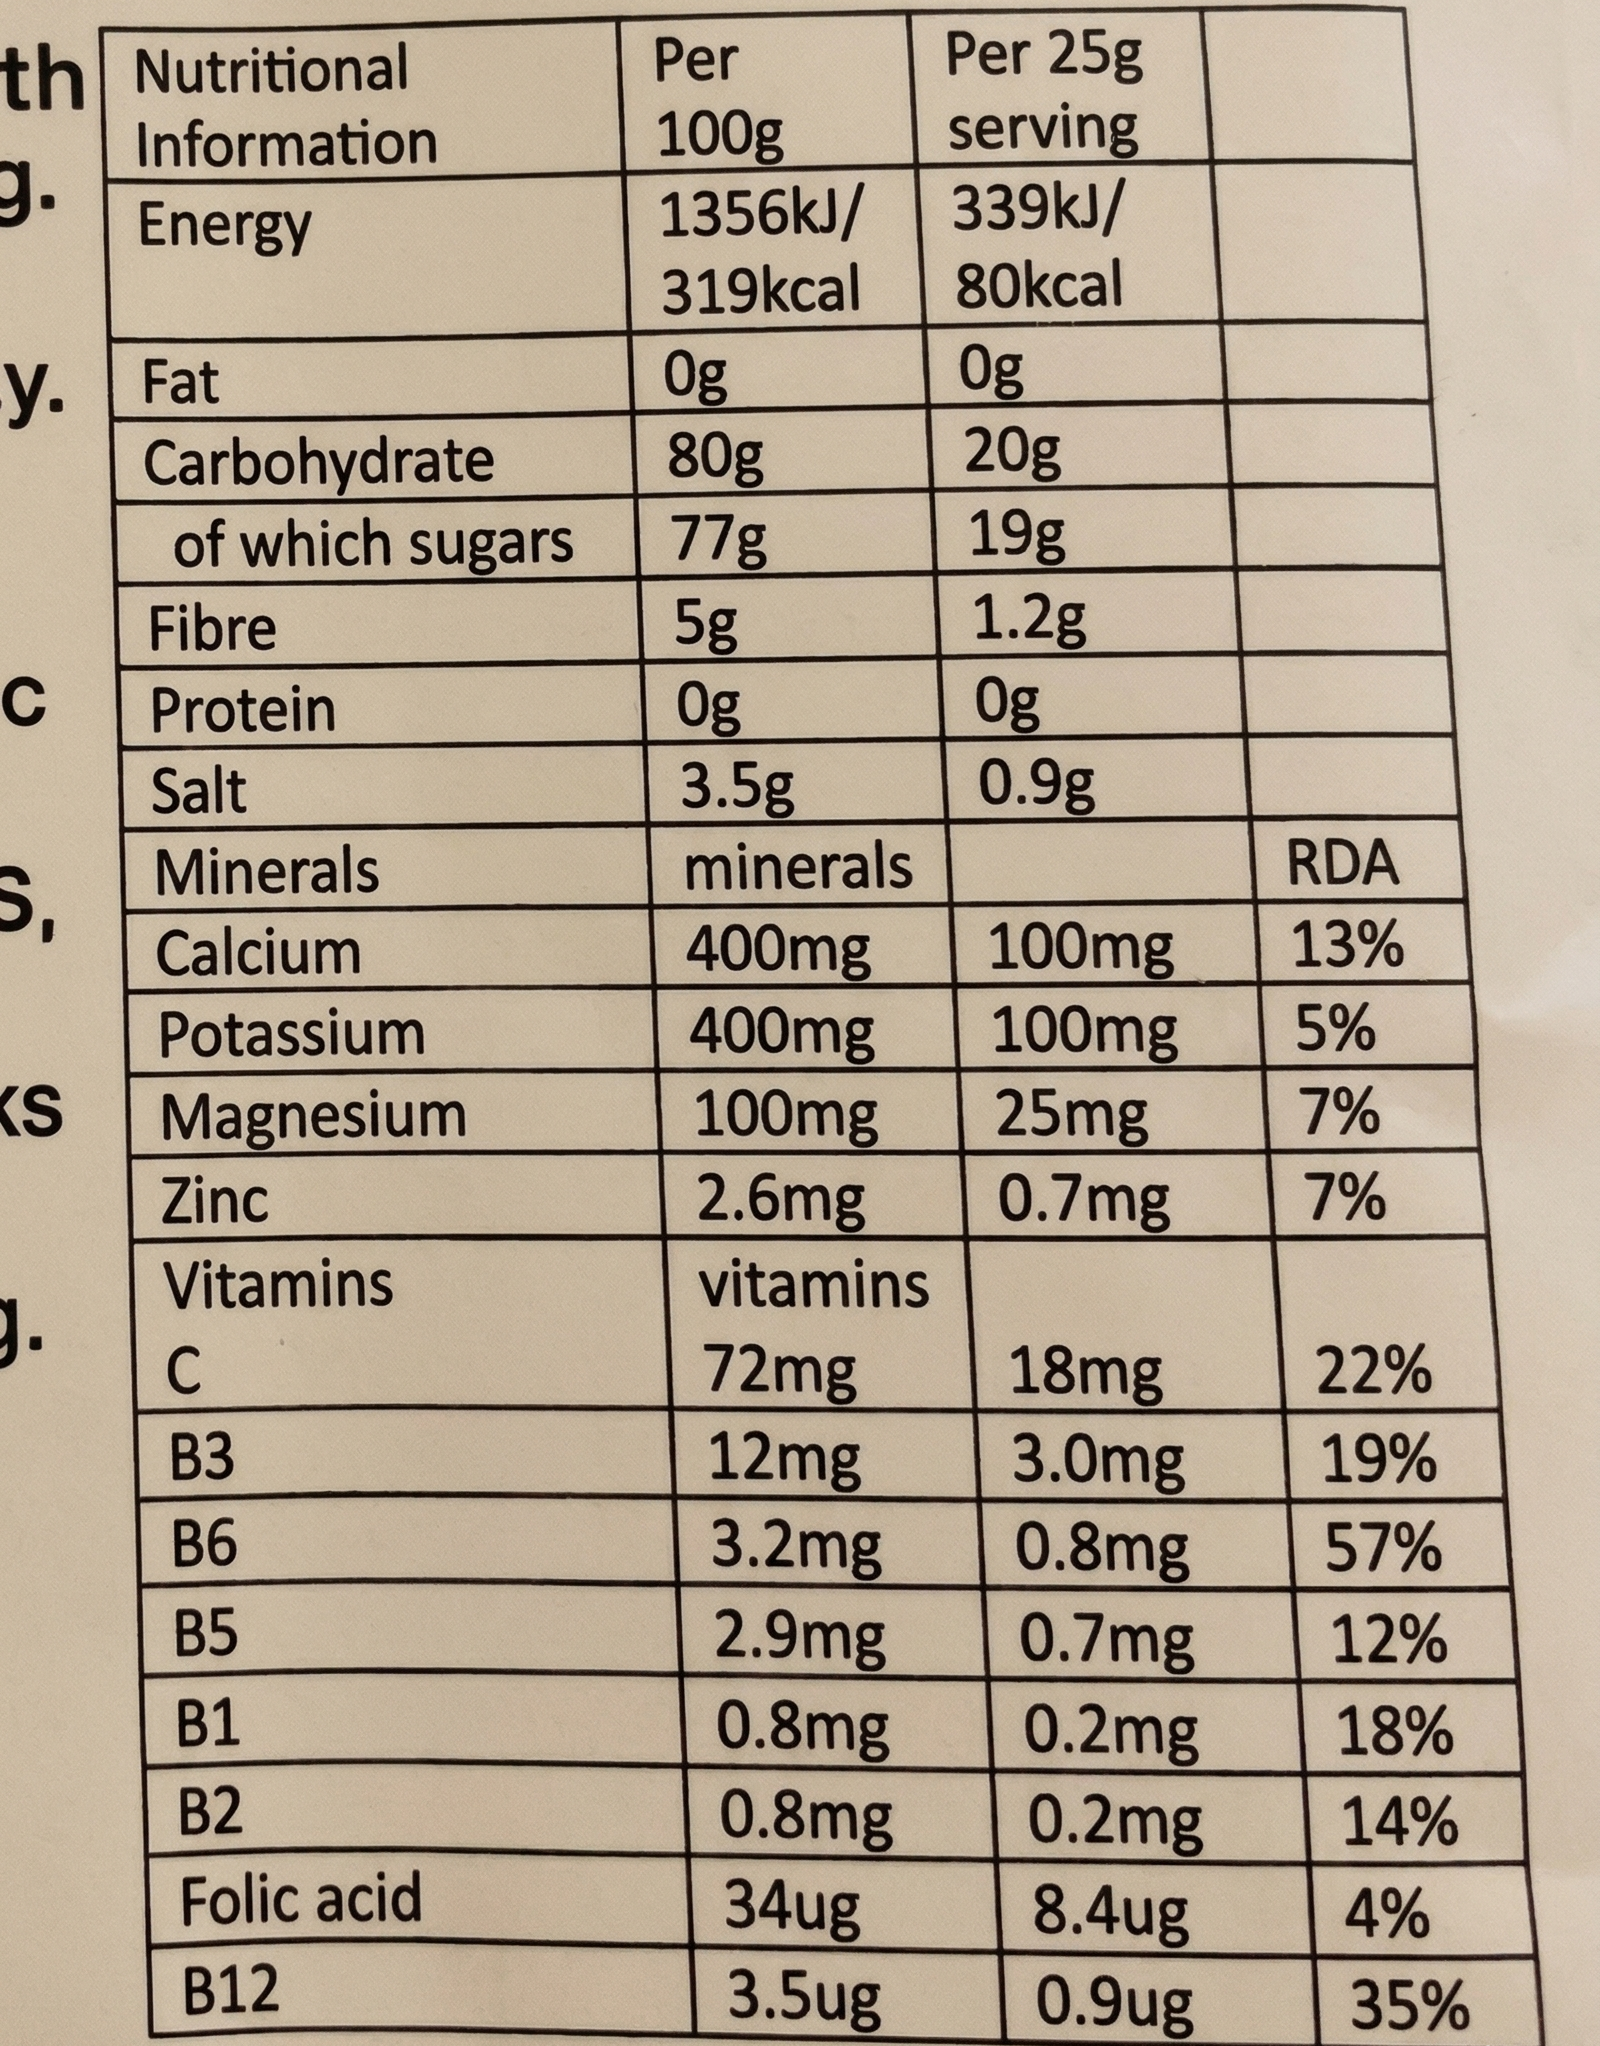
\includegraphics[width=0.60\linewidth,keepaspectratio]{34.png}
  \caption[Image 34: a two-context supplement label]{Image~34. Each nutrient is
    listed once per 100\,g and once per 25\,g serving, so the label has two value
    columns under one column of names. This is the layout where graph~v2's
    \mcode{HEADER_SCOPE} edge keeps the two contexts apart and graph~v1's single
    context edge does not.}
  \label{fig:example34-label}
\end{figure}

Table~\ref{tab:example34} shows the output of the two graph engines on this
label. For every nutrient it marks which of the two contexts each engine
recovers with all four fields correct. Graph~v1 recovers 15 of the 40 tuples,
while graph~v2 recovers 30, exactly double.

\begin{table}[htbp]
  \centering
  \caption[Worked example: correct tuples on image 34]{Correct four-field tuples
    on image~34, by nutrient and context. A check mark means the engine recovers
    that tuple with nutrient, quantity, unit, and context all correct; a blank
    cell means it does not. Each context has 20 gold tuples. Graph~v2 fills both
    columns, while graph~v1 recovers the per-100\,g column but none of the
    per-serving column.}
  \label{tab:example34}
  \small
  \begin{tabular}{@{}lcccc@{}}
    \toprule
     & \multicolumn{2}{c}{\textbf{Per 100\,g}} & \multicolumn{2}{c}{\textbf{Per 25\,g serving}} \\
    \cmidrule(lr){2-3}\cmidrule(lr){4-5}
    \textbf{Nutrient} & \textbf{v1} & \textbf{v2} & \textbf{v1} & \textbf{v2} \\
    \midrule
    Energy (kJ)      &            &            &            &            \\
    Energy (kcal)    &            &            &            &            \\
    Fat              &            & \checkmark &            &            \\
    Carbohydrate     & \checkmark & \checkmark &            & \checkmark \\
    Sugars           & \checkmark & \checkmark &            & \checkmark \\
    Fibre            & \checkmark & \checkmark &            & \checkmark \\
    Protein          & \checkmark & \checkmark &            &            \\
    Salt             & \checkmark & \checkmark &            & \checkmark \\
    Calcium          & \checkmark & \checkmark &            & \checkmark \\
    Potassium        & \checkmark & \checkmark &            & \checkmark \\
    Magnesium        & \checkmark & \checkmark &            & \checkmark \\
    Zinc             & \checkmark & \checkmark &            & \checkmark \\
    Vitamin C        & \checkmark & \checkmark &            & \checkmark \\
    Niacin           & \checkmark & \checkmark &            & \checkmark \\
    Vitamin B6       & \checkmark & \checkmark &            & \checkmark \\
    Pantothenic Acid & \checkmark & \checkmark &            & \checkmark \\
    Vitamin B1       & \checkmark & \checkmark &            & \checkmark \\
    Vitamin B2       & \checkmark & \checkmark &            & \checkmark \\
    Folic Acid       &            &            &            &            \\
    Vitamin B12      &            &            &            &            \\
    \midrule
    \textbf{Recovered (of 20)} & \textbf{15} & \textbf{16} & \textbf{0} & \textbf{14} \\
    \bottomrule
  \end{tabular}
\end{table}

The pattern is clear. On the per-100\,g column the two engines are almost the
same, 15 against 16. On the per-serving column graph~v1 recovers nothing at all,
while graph~v2 recovers 14. Graph~v1 does not fail on the numbers themselves; on
the first column it reads and binds them as well as graph~v2. It fails because
its single \mcode{CONTEXT_SCOPE} edge folds the label into one context, so the
whole per-serving column is left without a correct context and every tuple in it
is lost. Graph~v2 keeps the two columns apart with the \mcode{HEADER_SCOPE} edge
of Section~\ref{sec:graph-v2}, tying each value to the header of its own column,
so the 14 serving tuples are recovered. The gain is not better reading, but
keeping the second context alive.

The same behaviour holds across the whole multi-context set
(Table~\ref{tab:graph-context}); image~34 simply makes it visible. Almost the
entire advantage of graph~v2 on this label is the per-serving column that
graph~v1 drops.

The conclusion of this part of the axis is that graph~v2 is the stronger
association engine, and its advantage is structural: it attaches the
correct context in labels that report nutrients under more than one
reference basis, which graph~v1 cannot do.



\begin{figure}[t]
  \centering
  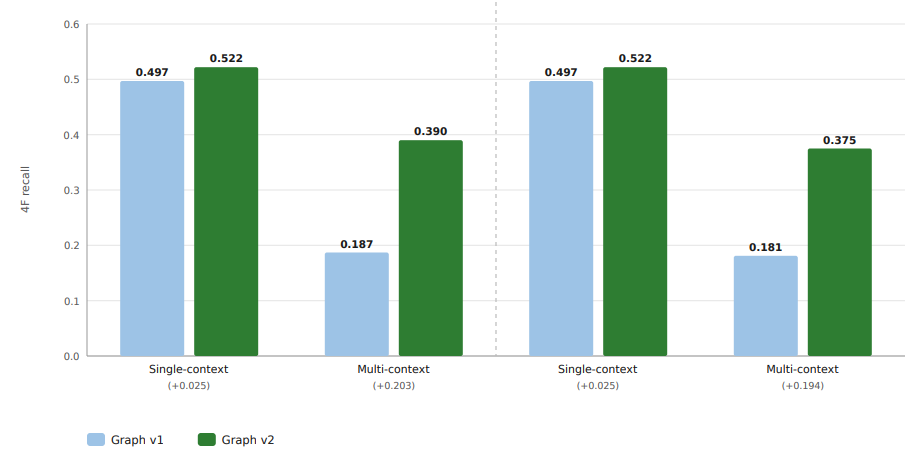
\includegraphics[width=1.2\linewidth,keepaspectratio]{graph_context_bars.png}
  \caption[Graph v1 vs graph v2: recall by context multiplicity]{Four-field
    recall of graph~v1 and graph~v2 on single-context images (159 tuples)
    and multi-context images (707 tuples), for both learned classifiers,
    OCR fixed and \mcode{overlap} edge mode. On single-context images the
    two engines are nearly equal; on multi-context images graph~v2 nearly
    doubles graph~v1. The whole advantage of graph~v2 is on multi-context
    labels.}
  \label{fig:graph-context-bars}
\end{figure}


% =====================================================================
%  6.5  ASSOCIATION AXIS — VLM FOR ASSOCIATION ONLY
% =====================================================================
\section{Vision--Language Model for Association}\label{sec:exp-vlm}

The fourth question has two parts. The pipeline can replace the graph with
a vision--language model at the association step only, as described in
Section~\ref{sec:vlm-assoc}. The first part asks whether this is better
than the graph. The second part asks whether it is better than letting a
vision--language model do the whole task end to end. OCR is fixed to
PaddleOCR and the classifier is held constant, so only the association
step changes. The three VLM-association runs are A\_VLM (rule-based),
E3-EMB-VLM (embedding), and E3-GLiNER-VLM (GLiNER); the end-to-end model
is E4.

\subsection{Versus the graph}\label{sec:exp-vlm-graph}

Table~\ref{tab:vlm-vs-graph} compares graph~v2 with the VLM-association
variant for each classifier. The VLM gives the higher four-field F1 in all
three cases, but the size of the gain differs: 0.4231 to 0.4819 for the
rule-based classifier, 0.4025 to 0.4945 for embedding, and 0.4304 to
0.4446 for GLiNER.

\begin{table}[htbp]
  \centering
  \caption[VLM association versus graph v2]{Graph~v2 against
    VLM-association for each classifier, OCR fixed to PaddleOCR. Scores are
    the four-field tuple as precision, recall, and F1. The VLM raises
    precision in every case while recall stays about the same.}
  \label{tab:vlm-vs-graph}
  \small
  \begin{tabular}{@{}llccc@{}}
    \toprule
    \textbf{Classifier} & \textbf{Association} & \textbf{4F-P} & \textbf{4F-R} & \textbf{4F-F1} \\
    \midrule
    Rule-based & Graph v2 (E2-A)        & 0.4223 & 0.4238 & 0.4231 \\
    Rule-based & VLM (A\_VLM)           & 0.5732 & 0.4157 & 0.4819 \\
    \addlinespace
    Embedding  & Graph v2 (E2-B)        & 0.3911 & 0.4145 & 0.4025 \\
    Embedding  & VLM (E3-EMB-VLM)       & 0.6054 & 0.4180 & 0.4945 \\
    \addlinespace
    GLiNER     & Graph v2 (E2-C)        & 0.4634 & 0.4018 & 0.4304 \\
    GLiNER     & VLM (E3-GLiNER-VLM)    & 0.5269 & 0.3845 & 0.4446 \\
    \bottomrule
  \end{tabular}
\end{table}

The table shows where the gain comes from. In every case recall stays
within two points, while precision rises sharply: by 15 points for the
rule-based classifier, 21 points for embedding, and 6 points for GLiNER.
The whole improvement is in precision. The reason is that the graph binds
whatever candidates it is given and does not re-check them, whereas the
vision--language model judges each binding against the token table and the
image and drops the ones it cannot justify. This removes false-positive
tuples that the graph keeps. The effect is largest for the embedding
classifier, which feeds the most non-nutrient candidates into association:
its precision rises the most, from 0.3911 to 0.6054. For GLiNER, which
already produces a clean candidate set, there is little for the model to
remove, so its gain is the smallest.

This also changes which classifier is best. Under graph~v2 the order is
GLiNER first, then rule-based, then embedding. Under VLM-association the
order reverses at the top: embedding first at 0.4945, then rule-based at
0.4819, then GLiNER at 0.4446. The embedding classifier has the highest
recall of the three learned candidate sets but the lowest precision. Under
the graph that low precision is a problem, because the surplus candidates
become false-positive tuples. Under the vision--language model the same
recall becomes an advantage, because the model keeps the extra correct
nutrients and removes the wrong ones. The best classifier therefore
depends on the association engine: GLiNER with the graph, embedding with
the model.

\subsection{Versus the end-to-end model}\label{sec:exp-vlm-e2e}

The second part compares the VLM-association runs with the end-to-end model
E4, which receives the label image and produces the tuples directly,
without the OCR and classification front-end. Table~\ref{tab:vlm-vs-e2e}
gives the four-field scores. All three VLM-association runs beat the
end-to-end model. The best, E3-EMB-VLM at 0.4945, is 0.135 above E4 at
0.3597.

\begin{table}[htbp]
  \centering
  \caption[VLM association versus the end-to-end model]{The three
    VLM-association runs against the end-to-end model E4. Scores are the
    four-field tuple as precision, recall, and F1. Giving the model the OCR
    token table beats letting it map the image directly to tuples.}
  \label{tab:vlm-vs-e2e}
  \small
  \begin{tabular}{@{}lccc@{}}
    \toprule
    \textbf{Pipeline} & \textbf{4F-P} & \textbf{4F-R} & \textbf{4F-F1} \\
    \midrule
    End-to-end VLM (E4)              & 0.4228 & 0.3129 & 0.3597 \\
    \addlinespace
    Rule-based + VLM (A\_VLM)        & 0.5732 & 0.4157 & 0.4819 \\
    Embedding + VLM (E3-EMB-VLM)     & 0.6054 & 0.4180 & 0.4945 \\
    GLiNER + VLM (E3-GLiNER-VLM)     & 0.5269 & 0.3845 & 0.4446 \\
    \bottomrule
  \end{tabular}
\end{table}

The same model does the binding in both cases, so the difference is the
front-end. In the end-to-end run the model must read the text, decide the
roles, and bind the fields all at once. In the VLM-association runs the OCR
and classification stages have already produced a clean token table, and
the model only has to bind the tokens. The token table raises both
precision and recall: precision rises because the model is not also making
OCR errors, and recall rises because the front-end has already recovered
tokens the model would miss from the image alone. The interpretable
front-end therefore helps even when a black-box model does the
association.

The conclusion of the association axis is that VLM-association gives the
best tuple F1 of any configuration, above both the graph and the
end-to-end model. This comes at a cost in interpretability, because the
binding step is a black box: the best interpretable pipeline, E2-C with
graph~v2 and GLiNER at 0.4304, is about six points below the best
VLM-association run. This trade-off is taken up in
Section~\ref{sec:exp-synth}.

% =====================================================================
%  6.6  ASSOCIATION AXIS — BEST GRAPH V2 EDGE MODE
% =====================================================================
\section{Edge-Creation Mode for Graph v2}\label{sec:exp-edge}

\begin{figure}[htbp]
  \centering
  \IfFileExists{row_edge_over_image.png}{%
    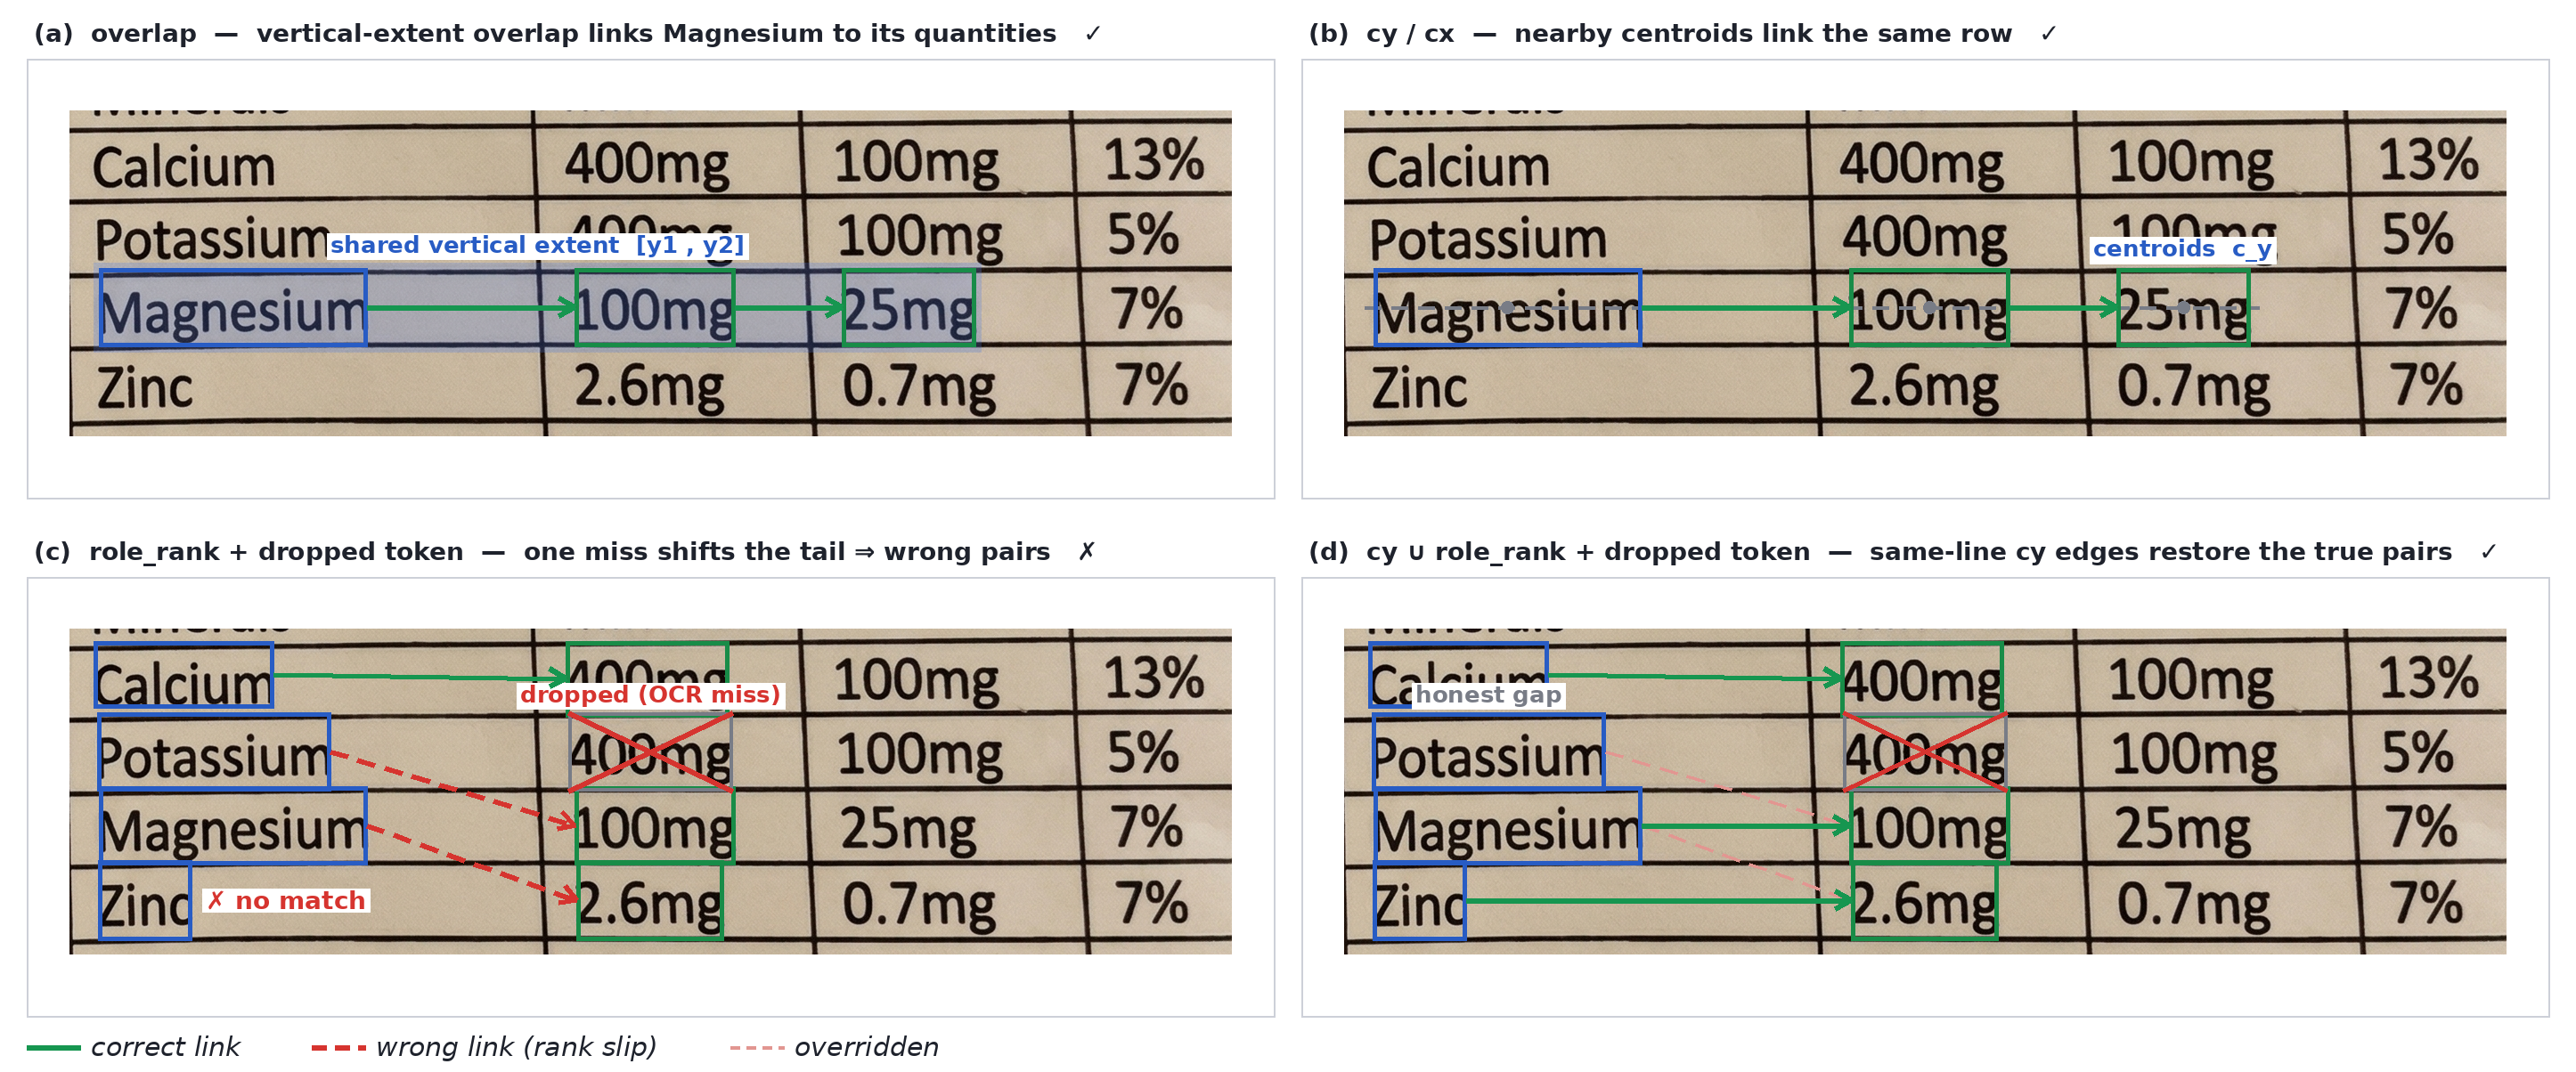
\includegraphics[width=\linewidth]{row_edge_over_image.png}%
  }{%
    \fbox{\parbox[c][45mm][c]{0.92\linewidth}{\centering\itshape
      Row-edge modes on a real label placeholder. Replace with
      \mcode{row_edge_over_image.png}.}}%
  }
  \caption[Row-edge modes on a real label]{%
    The four row-edge modes on a real label (34.png), where OCR has dropped
    Potassium's 400\,mg value. This is the real-data version of
    Figure~\ref{fig:row-modes}. (a)~and~(b) use geometry and pair each nutrient
    with its own quantities. (c)~uses rank order, so the missing value shifts
    the rest and pairs the wrong numbers. (d)~adds the geometric edges on top of
    the ranks and fixes the pairs again. Green is a correct link, red is a wrong
    one, and pink is a rank link that geometry overrides.}
  \label{fig:row-modes-real}
\end{figure}

The last question is which edge-creation mode builds the best row edges
inside graph~v2. The four modes defined in Section~\ref{sec:graph-v2} are
compared: the two geometric modes \mcode{overlap} and \mcode{cy-cx}, the
structural mode \mcode{role_rank}, and the union \mcode{cy}\,$\cup$\,\mcode{role_rank}.
OCR, the classifier, and the rest of graph~v2 are held fixed, so only the
row-edge rule changes. The sweep is run on the embedding classifier, which
covers all four modes, and is confirmed on GLiNER, which covers the two
geometric modes.

Table~\ref{tab:edge-modes} ranks the modes by four-field F1.

\begin{table}[htbp]
  \centering
  \caption[Graph v2 edge modes ranked by 4F-F1]{Graph~v2 edge-creation
    modes ranked by four-field tuple F1, with OCR and classifier fixed.
    The embedding rows cover all four modes; the GLiNER rows confirm the
    two geometric modes. \mcode{overlap} is best in both. All runs use the
    same deterministic evaluator (zero model calls), so the scores are
    directly comparable.}
  \label{tab:edge-modes}
  \small
  \begin{tabular}{@{}llc@{}}
    \toprule
    \textbf{Classifier} & \textbf{Edge mode} & \textbf{4F-F1} \\
    \midrule
    Embedding & \mcode{overlap}                  & 0.4025 \\
    Embedding & \mcode{cy-cx}                     & 0.3860 \\
    Embedding & \mcode{cy}\,$\cup$\,\mcode{role_rank}     & 0.3190 \\
    Embedding & \mcode{role_rank}                 & 0.1320 \\
    \addlinespace
    GLiNER    & \mcode{overlap}                   & 0.4304 \\
    GLiNER    & \mcode{cy-cx}                      & 0.4135 \\
    \bottomrule
  \end{tabular}
\end{table}

The ranking is the same for both classifiers. The geometric \mcode{overlap}
mode is best, the centre-based \mcode{cy-cx} mode is close behind, and the
two modes that use ordinal rank are worse. The structural \mcode{role_rank}
mode is the weakest by a wide margin, at 0.1320, because a single missed or
fused token shifts the rank order and breaks the row alignment, as
explained in Section~\ref{sec:enrichment-rowviews}. The union
\mcode{cy}\,$\cup$\,\mcode{role_rank} is also below the geometric modes, because
adding the rank-based edges to the geometric ones brings in wrong row links
rather than new correct ones. Geometric row edges are therefore the right
choice, and \mcode{overlap} is used as the default edge mode in every
graph~v2 run in this chapter.

\begin{figure}[t]
  \centering
  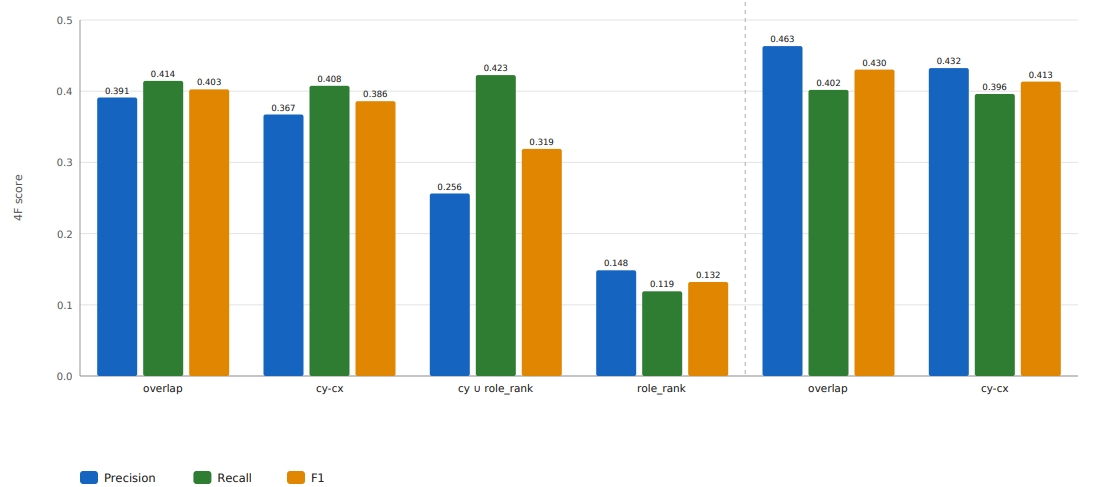
\includegraphics[width=1.15\linewidth,keepaspectratio]{edge_modes_bars.png}
  \caption[Graph v2 edge modes: precision, recall, and F1]{Four-field
    precision, recall, and F1 for the graph~v2 edge modes, with OCR and
    classifier fixed. The embedding sweep (left) covers all four modes; the
    GLiNER sweep (right) covers the two geometric modes. \mcode{overlap}
    has the highest F1 in both. The \mcode{cy}\,$\cup$\,\mcode{role_rank}
    mode has the highest recall in the embedding sweep but a much lower
    precision, showing that merging the rank-based edges adds tuples at the
    cost of precision; \mcode{role_rank} alone is weakest on all three
    metrics.}
  \label{fig:edge-modes-bars}
\end{figure}

% =====================================================================
%  6.7  CROSS-AXIS SYNTHESIS
% =====================================================================
\section{Cross-Axis Synthesis}\label{sec:exp-synth}

Each axis was settled on its own. Taken together, they show which choices
carried the result and which barely changed it. OCR stands apart from the
rest: PaddleOCR wins outright (Section~\ref{sec:exp-ocr}) and is used in
every run, so the questions that remain are the classifier and the
association engine, and those two pull against each other.

Figure~\ref{fig:effect-sizes} ranks the changes by how far each one moved
the four-field F1. Reading the text correctly matters most, and the switch
from EasyOCR to PaddleOCR is the largest jump of all. Next comes the move
from graph~v1 to graph~v2. The classifier moves the score least. So most of
the gain comes from reading the tokens and binding them with the better
graph; the classifier is a smaller adjustment on top.

\begin{figure}[t]
  \centering
  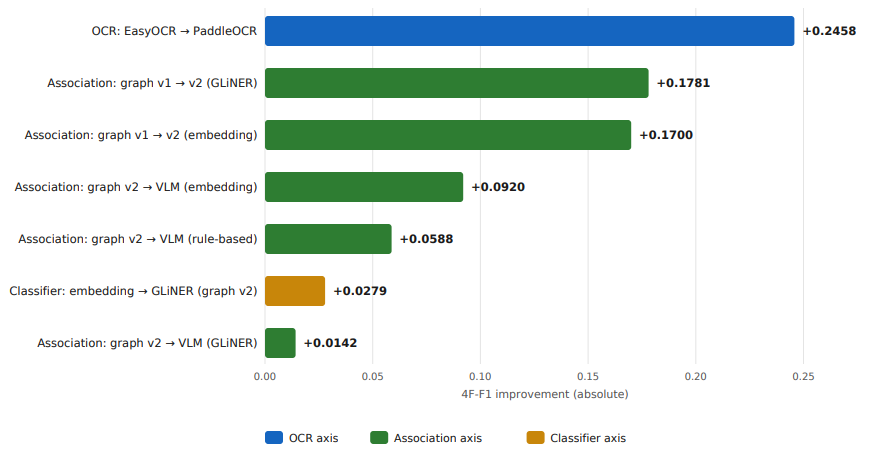
\includegraphics[width=1.15\linewidth,keepaspectratio]{effect_sizes.png}
  \caption[Effect of each pipeline change on 4F-F1]{Effect of each pipeline
    change on the four-field tuple F1. Each bar is the change from one
    substitution, with every other stage fixed. The OCR engine is the
    largest single factor, the move from graph~v1 to graph~v2 is next, and
    the classifier choice is the smallest.}
  \label{fig:effect-sizes}
\end{figure}

The runs also fall into three tiers, set by how much of the pipeline can be
inspected. In Tier~1 every stage is a rule or a graph, including the step
that turns tokens into tuples. Tier~2 keeps the upstream stages and swaps
only the binding step for a vision--language model. Tier~3 keeps no
structure at all: the image goes straight to a vision--language model and
the tuples come back. Table~\ref{tab:tiers} gives the best run in each.

\begin{table}[htbp]
  \centering
  \caption[Three interpretability tiers]{The three interpretability tiers
    and the best run in each. Tier~1 uses no black box at any stage.
    Tier~2 keeps the interpretable upstream stages and replaces only the
    association step with a vision--language model. Tier~3 hands the raw
    image to a vision--language model and reads the tuples directly from
    its output. The score is four-field tuple F1.}
  \label{tab:tiers}
  \small
  \begin{tabular}{@{}llc@{}}
    \toprule
    \textbf{Tier} & \textbf{Best run} & \textbf{4F-F1} \\
    \midrule
    Tier~1 --- fully interpretable                 & E2-C (GLiNER, graph~v2)            & 0.4304 \\
    Tier~2 --- interpretable upstream, VLM assoc.   & E3-EMB-VLM (embedding, VLM assoc.) & 0.4945 \\
    Tier~3 --- fully black-box end-to-end          & E4 (end-to-end VLM)                & 0.3597 \\
    \bottomrule
  \end{tabular}
\end{table}

How the tiers rank is the main result of the chapter. Tier~2 comes
first---E3-EMB-VLM reaches 0.4945, with the interpretable upstream stages
feeding a model that only has to bind. The fully interpretable Tier~1 run,
E2-C, follows at 0.4304. Last is the black-box Tier~3 run, E4, at 0.3597.
Two points stand out. The structured pipeline beats the raw model by about
seven points, so shaping the problem before binding any field clearly pays
off. And the only runs that beat the interpretable pipeline keep their
upstream stages and change one step, so the extra points come from the
binding step alone---and they cost interpretability.

Different goals favour different runs, as Table~\ref{tab:best-by-objective}
shows.

\begin{table}[htbp]
  \centering
  \caption[Best configuration by objective]{Best configuration for each
    objective, over all runs in this chapter. The metric shown is the one
    the objective names; all values are four-field tuple scores.}
  \label{tab:best-by-objective}
  \small
  \begin{tabular}{@{}llc@{}}
    \toprule
    \textbf{Objective} & \textbf{Best configuration} & \textbf{Score} \\
    \midrule
    Highest tuple F1 (overall)       & E3-EMB-VLM (embedding, VLM assoc.) & 0.4945 \\
    Highest tuple F1 (interpretable) & E2-C (GLiNER, graph~v2)            & 0.4304 \\
    Highest tuple precision          & E3-EMB-VLM (embedding, VLM assoc.) & 0.6054 \\
    Highest tuple recall             & E2-A (rule-based, graph~v2)        & 0.4238 \\
    \bottomrule
  \end{tabular}
\end{table}

E3-EMB-VLM has the best F1 and the best precision. Recall peaks with E2-A,
the rule-based graph run, which recovers the most correct tuples but admits
enough wrong ones to fall well behind on precision. For a fully
interpretable system, E2-C is the pick. No run leads on every measure, so
the choice follows whatever the task values most.

The classifier and the association engine interact in a tidy way. Put
GLiNER with the graph and the interpretable score is best: GLiNER is
precise, so few wrong candidates ever reach the graph (E2-C, 0.4304). Put
the embedding classifier with the vision--language model and the overall
score is best: of the learned classifiers it finds the most nutrients, and
the model discards the wrong bindings its extra candidates would otherwise
produce (E3-EMB-VLM, 0.4945). Either way, the rule-based classifier sits in
the middle. There is no single best classifier; the right one depends on
what does the binding.

\begin{figure}[t]
  \centering
  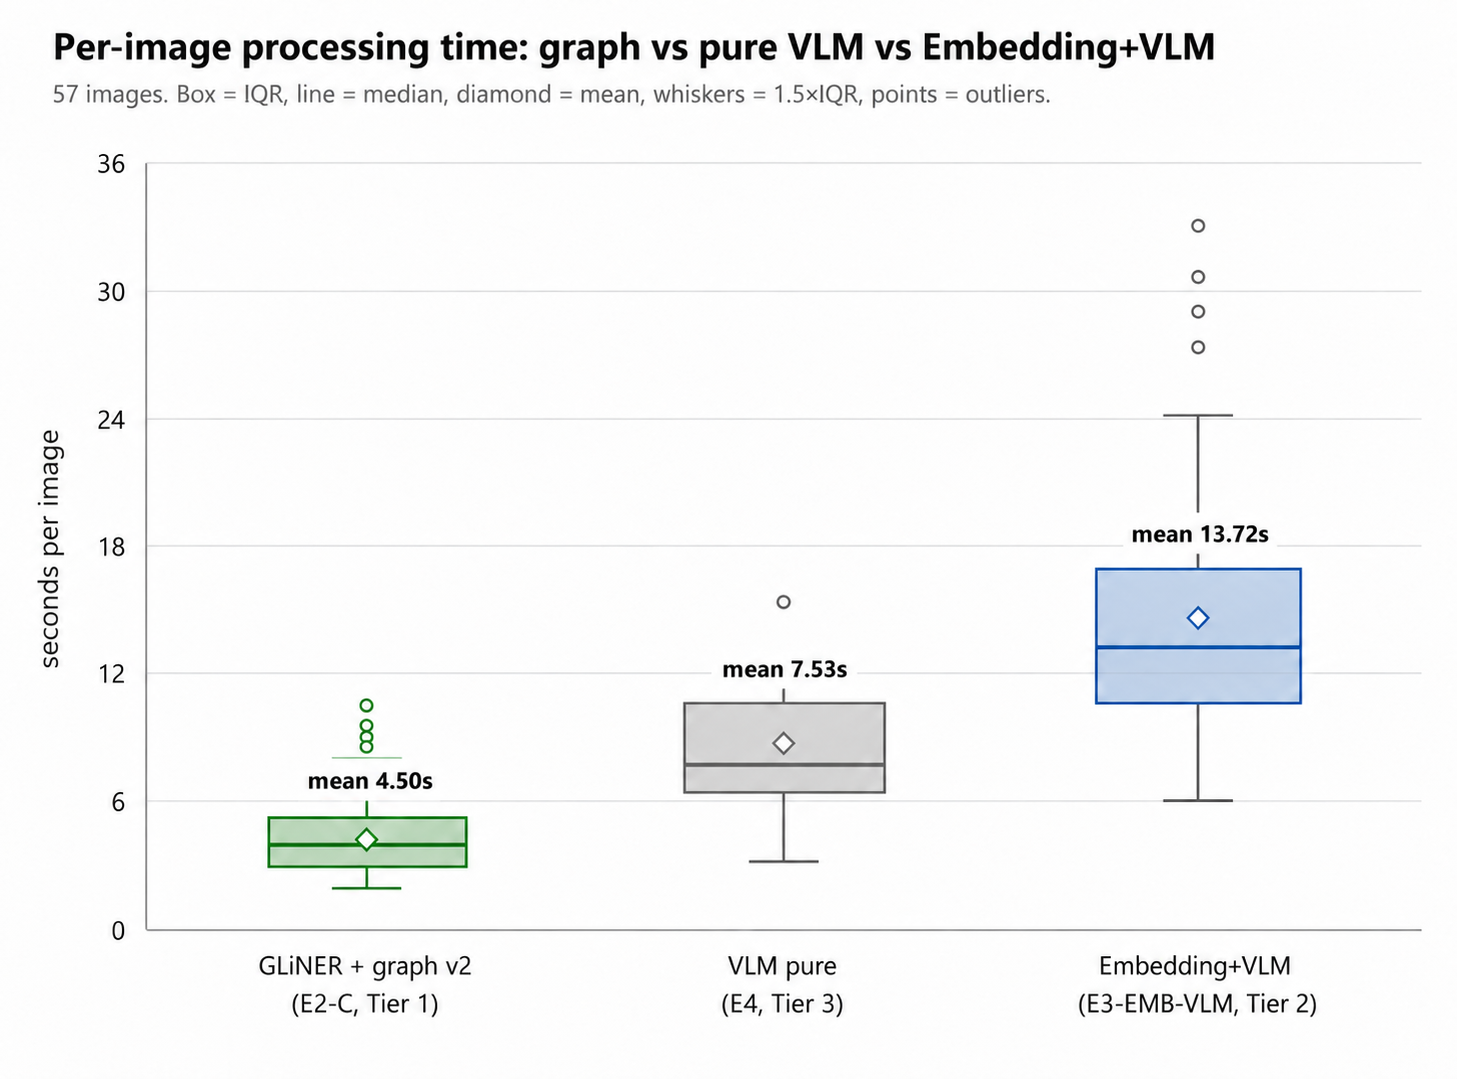
\includegraphics[width=\linewidth,keepaspectratio]{per_image_runtime.png}
  \caption[Per-image processing time by tier]{Per-image processing time for
    the three tiers, over the 57 test images. The box is the interquartile
    range, the line the median, and the diamond the mean. The interpretable
    pipeline (E2-C) is fastest, the end-to-end model (E4) sits in between,
    and the embedding-plus-VLM hybrid (E3-EMB-VLM) is the slowest.}
  \label{fig:runtime}
\end{figure}

Cost separates the runs as sharply as score does.
Figure~\ref{fig:runtime} gives the per-image time for the three tiers. The
interpretable pipeline is fastest, at a mean of 4.50 seconds, because it
never calls the model. The pure end-to-end run sits in the middle at 7.53
seconds. Slowest is the embedding-plus-VLM hybrid at 13.72 seconds---about
three times the interpretable pipeline---since it runs the full upstream
pipeline and then adds a model pass. The best-scoring run is therefore also
the most expensive. That model pass is likewise the step that cannot be
read back, where the graph binds by a rule one can inspect. So the points
won by VLM-association are paid three ways: in runtime, in compute, and in
interpretability. Which configuration fits depends on the time budget and
on whether the binding step must be inspectable.
Section~\ref{sec:exp-error} turns to the errors that remain in every
configuration and where they begin.

% =====================================================================
%  6.8  ERROR ANALYSIS
% =====================================================================
\section{Error Analysis}\label{sec:exp-error}

This section looks at where tuples are lost. It uses the best interpretable
run, E2-C (GLiNER with graph~v2), because every stage in it is a rule or a
graph and the losses can be followed step by step; the runs that bind with
the vision--language model hide that step inside a model that cannot be read
back. The losses traced here sit before the binding step, so the runs that
share the same OCR and classifier carry them too.

Table~\ref{tab:funnel} follows the 866 gold tuples through the run. The
nutrient is matched for 552 of them, and 348 of those come out fully
correct. Two losses remain. The larger one is the 314 tuples whose nutrient
is never matched---about a third of the gold set is gone before any field is
attempted. The smaller one is the 204 tuples that match on the nutrient but
get at least one field wrong. Separately, 199 of the 751 predicted tuples
match no gold nutrient at all, and these drag precision down.

\begin{table}[htbp]
  \centering
  \caption[Where the gold tuples go]{Where the gold tuples go under the best
    interpretable run, E2-C (GLiNER, graph~v2), on the full test set (866
    tuples, 57 images) and the reduced set (820~tuples, 55~images) with
    images 15 and 67 removed. A tuple is nutrient-matched when its nutrient
    is paired with a prediction; the fully correct ones have all four fields
    right. The false positives are predicted tuples that match no gold
    nutrient. The analysis in this section reads the full set.}
  \label{tab:funnel}
  \small
  \begin{tabular}{@{}lcc@{}}
    \toprule
    \textbf{Outcome} & \textbf{Full (866)} & \textbf{Reduced (820)} \\
    \midrule
    Gold tuples                            & 866 & 820 \\
    Nutrient matched                       & 552 & 543 \\
    \quad fully correct (all four fields)  & 348 & 339 \\
    \quad one or more fields wrong         & 204 & 204 \\
    Nutrient not matched (recall loss)     & 314 & 277 \\
    \addlinespace
    Predicted tuples                       & 751 & 742 \\
    \quad false positives (no gold match)  & 199 & 199 \\
    \midrule
    Four-field precision                   & 0.4634 & 0.4569 \\
    Four-field recall                      & 0.4018 & 0.4134 \\
    Four-field F1                          & 0.4304 & 0.4341 \\
    \bottomrule
  \end{tabular}
\end{table}




The 204 partial failures do not fall evenly on the four fields. After the
nutrient is matched, context is read most reliably and quantity least: the
per-field accuracies are 87.9, 83.2, and 76.3 percent for context, unit,
and quantity (Section~\ref{sec:exp-classifier}). Quantity is the weak field,
wrong on 131 of the 552 matched tuples. Reading a number and tying it to the
right nutrient is simply harder than reading a short unit or a column
header.

Three patterns produce most of these losses. Some images defeat the OCR
outright: on 68.jpeg the text returns corrupted, and 67.jpeg is a
pharmaceutical label the engine reads poorly, so their 34 and 4 gold tuples
fall at the nutrient stage. Others defeat the table logic rather than the
OCR---15.PNG lays its 42 values out in running paragraphs instead of a
table, and only the paragraph fallback recovers any of them.
(Images 15 and
67 are the two later removed from the primary test set, as noted in
Chapter~\ref{chap:evaluation};they are discussed here because this analysis
is run on the full 866-tuple set.) The rest is the
quantity misalignment behind the weak quantity field. The value columns are
separated and labelled in the enrichment stage, and on dense tables that
place two value columns side by side, as 118.jpeg and 119.jpeg do across
their 40 gold tuples, that stage can place a value in the wrong column---so
a per-serving number is bound where the per-100\,g number belongs.

Two limits therefore bound the interpretable pipeline: the recall ceiling
set by what the OCR and classifier recover, and the column misalignment that
mis-binds quantities on dense tables. Both arise before the binding step.
The graph cannot repair either, since it binds from the columns and tokens
it is handed. The vision--language model lifts precision---with the
classifier held fixed, swapping the graph for the model barely moves recall
(embedding, 0.4145 to 0.4180)---but the nutrients missed upstream stay
missed. Section~\ref{sec:exp-summary} brings the chapter's findings
together.


% =====================================================================
%  DISTANCE-BASED LINKING VALIDATION
%  (placement: new section after Section~\ref{sec:exp-error} (Error Analysis),
%   i.e. the new 6.9, with Summary of Findings becoming 6.10)
%  Figure file: fig_below_above_split.png  (the two-panel below/above chart)
% =====================================================================
\section{Distance-Based Linking Validation}\label{sec:exp-distance}

Section~\ref{sec:exp-edge} showed that geometric row edges work better than
rank-based ones. This section checks the same idea in a simpler way. When we
join a nutrient to a quantity, how far apart are their boxes on the label?
And can this distance tell a good link from a bad one? The test uses the
PaddleOCR front-end, and it does not change any score in this chapter.

First, we need to say which pairs are allowed. We use the same idea as the
error analysis (Section~\ref{sec:exp-error}): the OCR usually loses
quantities, but it reads nutrient names well. Suppose only quantities are
lost. Then the list of nutrients stays complete and in order. When a quantity
is lost, the quantities under it move up. So a nutrient can never take a
quantity that comes before it. It can only take its own quantity or one that
comes later. In rank terms, a nutrient at rank~$k$ is joined to every quantity
at rank~$k$ or larger, where rank means the top-to-bottom order. If no
quantity is lost, this is just rank~$k$ to rank~$k$.

For each pair, we draw a vector from the middle of the nutrient box to the
middle of the quantity box. The average is then worked out for each image on
its own: we take all the vectors on that one image and find their average, so
every image has its own average vector. Inside an image, we also do this column
by column, so a per-100\,g column and a per-serving column are not mixed. Every vector is then longer or shorter
than this average. Figure~\ref{fig:displacement-belowabove} shows the two
counts for each label. On the 55 labels, 4{,}605 pairs were made. Almost half
are below the average (2{,}119, or 46\%), and a little more than half are above
it (2{,}486, or 54\%). Some labels have fewer than two quantities. Then no
column can be made, so the label is left out. These are the empty places in the
figure (78.jpeg, 111.jpeg and 112.jpeg; 15.png and 67.jpeg were removed
earlier).

\begin{figure}[t]
  
  \makebox[\linewidth][c]{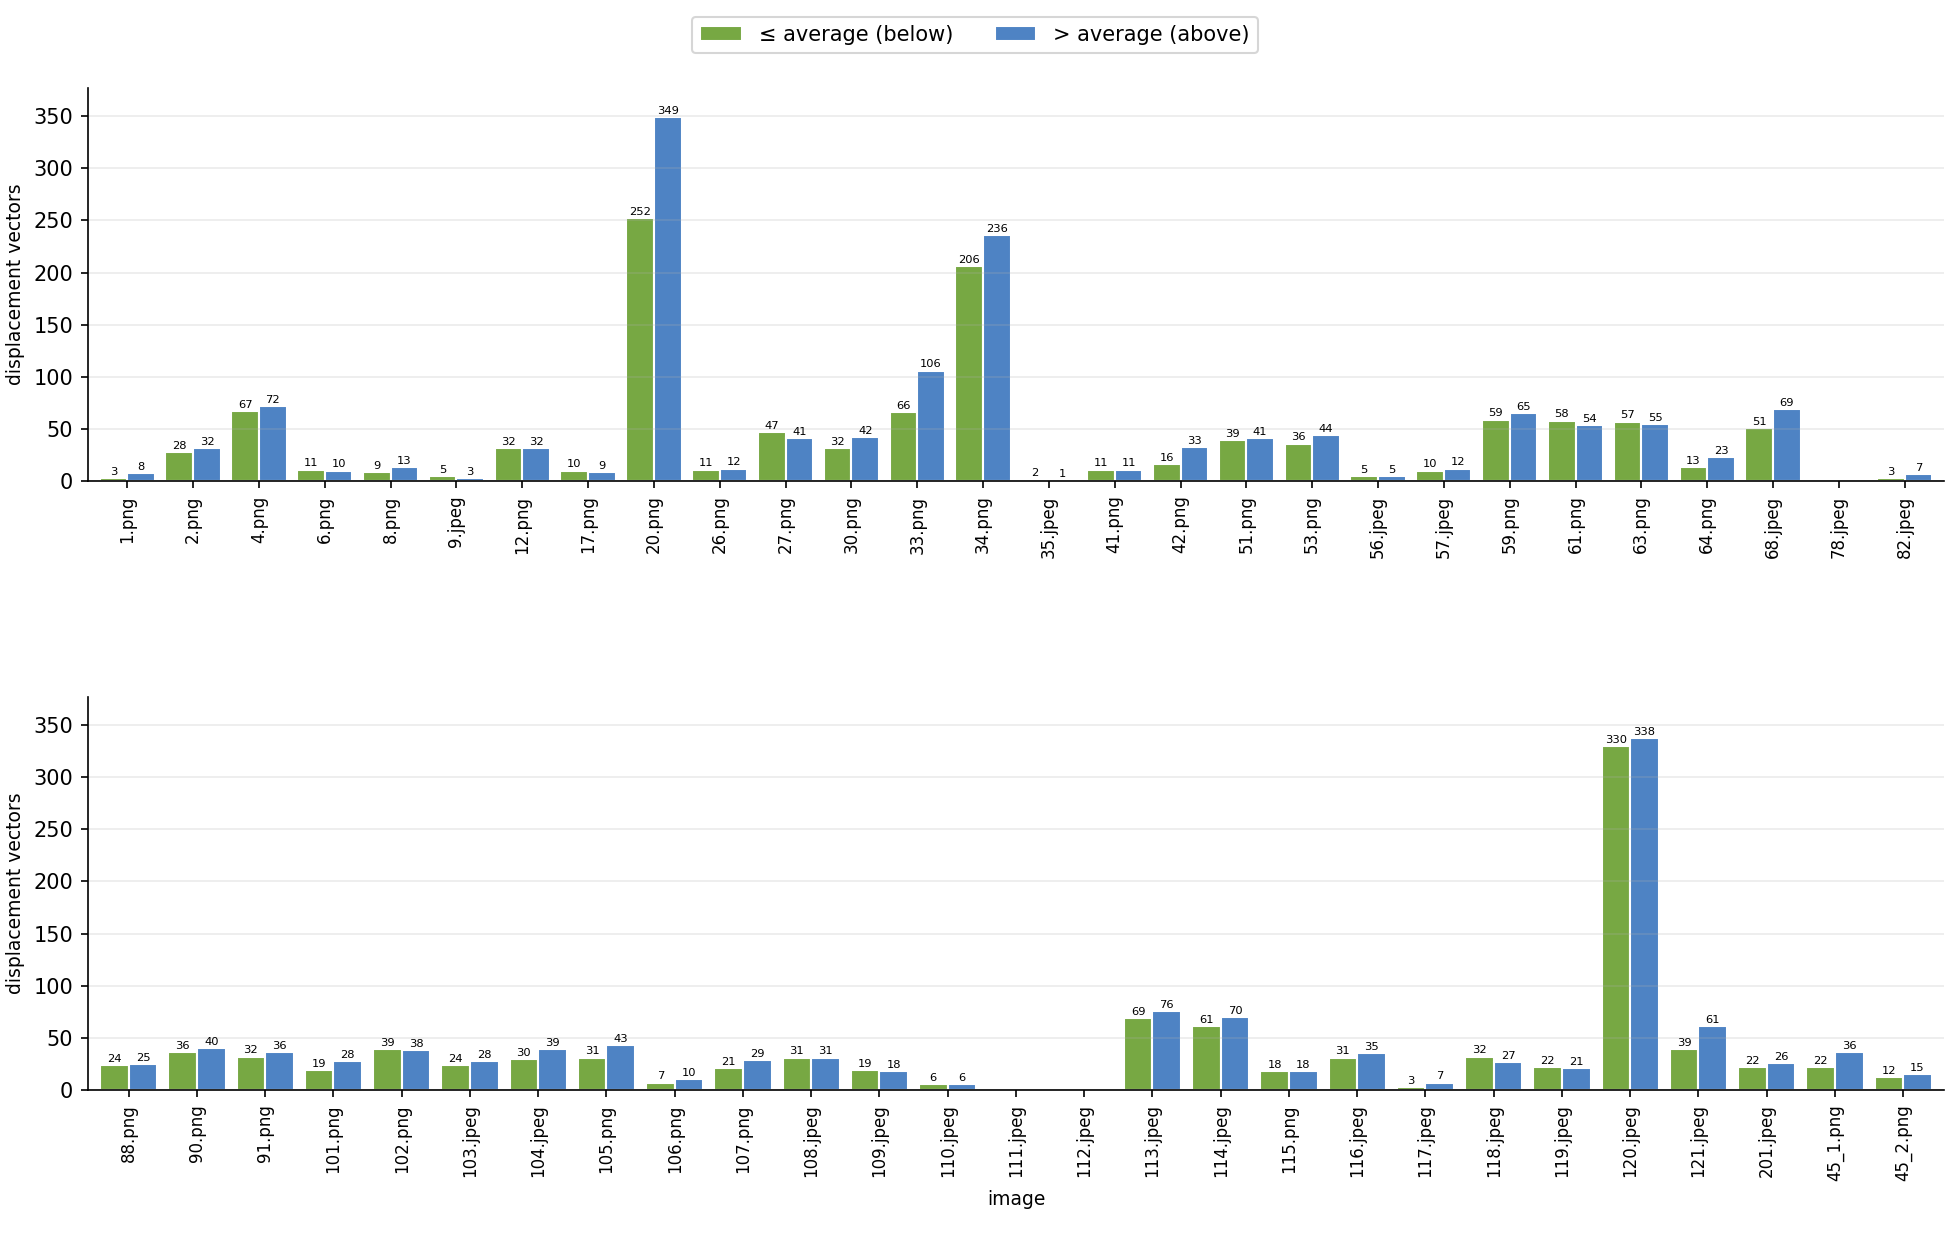
\includegraphics[width=1.4\linewidth,keepaspectratio]{fig_below_above_split.png}}
  \caption[Displacement vectors below and above the image average]{%
    For each label, the number of vectors that fall below (green) and above
    (blue) that label's own average vector. A pair is one possible
    nutrient--quantity link, measured from the middle of the nutrient box to
    the middle of the quantity box. Empty places are labels with too few
    quantities to make a pair. The 55 labels are shown in two rows so they are
    easier to read.}
  \label{fig:displacement-belowabove}
\end{figure}

Two things come out of this. First, real links sit in a steady place. On every
label the horizontal part of the average vector is large, because the quantity
is to the right of the name, and the vertical part is small. So a real pair has
a short and stable gap. This says the same thing as Section~\ref{sec:exp-edge},
but without the tuple score: what keeps a link together is position, not order.
Second, the distance finds many links but cannot pick between them. On the two
fields it can check---the nutrient and its value---the below-average pairs
cover 366 of the 866 gold links (42\%). This is close to the 421 (49\%) that
the full pipeline with the \mcode{overlap} edge mode reaches on the same two
fields (Section~\ref{sec:exp-error}).
But the split in Figure~\ref{fig:displacement-belowabove} is almost even. A
real link is about as likely to be above the average as below it. So the
distance only suggests good pairs; it does not choose them. This is why the
association stage joins them with the geometric edges of
Section~\ref{sec:graph-v2}, and not with a simple distance rule. One last
point: this measure cannot find missing values. A token that is never read has
no box, so it has no vector, and a lost quantity leaves no mark here at all.


% =====================================================================
%  6.9  SUMMARY OF FINDINGS
% =====================================================================
\section{Summary of Findings}\label{sec:exp-summary}

The chapter answered five questions by ablation, changing one stage at a
time. This section collects the answers.

OCR matters most. PaddleOCR beats EasyOCR on every field, and the gap is in
the values rather than the names: quantity, unit, and context each rise by
twenty-five to thirty points, while nutrient detection barely moves. The
four-field F1 climbs from 0.1773 to 0.4231 on the OCR change alone, so
PaddleOCR is used in every other run.

The association engine is the next-largest factor, and its design is where
the interpretable result is made. Graph~v2 nearly doubles the four-field F1
of graph~v1 for both learned classifiers, and the gain is structural: it
shows on the multi-context labels, the ones with more than one value column,
where graph~v1 cannot keep the columns apart. Inside graph~v2, geometric row
edges are the right choice---the \mcode{overlap} mode wins, the rank-based
modes are much weaker, and adding rank edges to the geometric ones only
brings in wrong links. The classifier is the smallest factor. It acts only
through nutrient detection, since the shared cascade reads quantity, unit,
and context the same way whichever classifier is used; among the zero-shot
options GLiNER gives the best interpretable tuple score, 0.4304, with no
curated lexicon.

That run, E2-C, is the best fully interpretable pipeline and the chapter's
main result. Replacing only the binding step with a vision--language model
raises the score further, to 0.4945, by lifting precision while recall
holds---and with the model doing the binding, the embedding classifier
overtakes GLiNER, reversing the order seen on the graph. Both of these beat
a vision--language model run end to end, which reaches only 0.3597, so
structuring the problem before any field is bound is worth more than handing
the whole task to one model. The extra points from the model are paid for in
interpretability and in time: the interpretable pipeline runs in about four
and a half seconds per image, the hybrid in about fourteen.

Two limits bound all of these configurations. About a third of the gold
tuples are lost because the nutrient is never read, a ceiling set by the OCR
and the classifier; and quantity is the weakest field, mis-bound on dense
tables where two value columns sit side by side. Both arise before the
binding step, so they pass through every run. What they suggest for the
design, and the work that remains, is taken up in the following chapter.                 % your filename

% ----------------------------------------------------------------------
% Chapter 7 — Discussion and Conclusion
% ----------------------------------------------------------------------
% !TEX root = thesis.tex
% =====================================================================
%  CHAPTER 7 — CONCLUSION
%  Zero-Shot Nutrient and Quantity Association using
%  OCR-Guided Semantic Graph Matching
%  Moustafa Hamada | THD + USB
%
%  Build: scrbook, XeLaTeX + BibTeX. Cross-refs: Chapter~\ref{} / Section~\ref{}.
%
%  This file DEFINES \label{chap:conclusion}, which resolves the forward
%  reference made from the Introduction (Chapter 1). Placed last in the
%  document, after Chapters 1--6.
%
%  BACK REFERENCES (labels already defined in the other chapter files):
%    chap:introduction (Ch1), chap:experiments (Ch6)
%
%  This chapter is high-level and adds NO new citations (it refers back to the
%  chapters where each component and result was introduced).
%
%  NOTE: \mcode{} is defined inside Chapter 4. In a full front-to-back build it
%  would be available here, but this chapter is kept free of \mcode so it also
%  compiles standalone; edge types and modes are named in plain words instead.
%
%  All figures for the four-field results (0.4304 / 0.4945 / 0.3597, the OCR
%  jump, the runtime split) are stated verbatim from the locked runs reported
%  in Chapter~\ref{chap:experiments}.
%
%  LABELS IN THIS FILE:
%    chap:conclusion
%    sec:concl-findings, sec:concl-limitations, sec:concl-future,
%    sec:concl-closing
% =====================================================================

\chapter{Conclusion}\label{chap:conclusion}

This thesis set out to reconstruct structured nutritional records from images of
supplement and food labels, under two demands that usually pull against each
other. The method had to work zero-shot, on labels, layouts, and languages it had
never seen, and it had to stay open to inspection at every stage rather than hand
the task to a single opaque model. The answer proposed and tested here is a
modular pipeline that reads the label with OCR, classifies each token into a
semantic role without training on the target labels, and then binds the tokens
into four-field tuples
$\langle\text{nutrient},\,\text{quantity},\,\text{unit},\,\text{context}\rangle$
by matching an explicit graph whose edges follow closed-form geometric and
structural rules. This chapter reviews what the pipeline achieved against the
questions set in Chapter~\ref{chap:introduction}, states where it falls short, and
points to the work that would take it further.

\section{Summary of Findings}\label{sec:concl-findings}

The experiments in Chapter~\ref{chap:experiments} answered each of the five
questions by ablation, changing one stage at a time. The reading stage proved to
be the single largest lever. Replacing EasyOCR with PaddleOCR PP-OCRv5, with every
later stage held fixed, lifted the four-field tuple F1 from 0.1773 to 0.4231, and
the gain came almost entirely from reading the numbers and units correctly rather
than from finding more nutrient names. Because OCR sets the ceiling for everything
after it, PaddleOCR was fixed for the rest of the work.

The association stage was the next-largest factor, and it is where the
contribution sits. The enriched, geometry-aware graph nearly doubled the
four-field F1 of the naive geometric graph for both learned classifiers, and the
gain was structural rather than a matter of better reading: it appeared almost
entirely on the multi-context labels, the ones that report the same nutrient under
more than one reference basis, where the header-scope relation keeps the value
columns apart and the simpler graph cannot. Inside the enriched graph, geometric
row edges were clearly the right mechanism. The geometric overlap mode was best,
the rank-based modes were far weaker --- a single missed or fused token shifts the
ordinal count and breaks the alignment --- and merging rank edges into the
geometric ones only added wrong links. This confirmed the central design choice:
on labels distorted by OCR, physical alignment is a more reliable basis for the
row relation than ordinal rank.

The classifier was the smallest of the three factors, because it acts only through
nutrient detection while the shared cascade reads quantity, unit, and context the
same way in every run. Among the zero-shot options, GLiNER-biomed gave the best
interpretable tuple score, and it did so without any hand-built lexicon, which
matters for a method that claims to generalise beyond a fixed vocabulary.

Taken together, these choices give the central result of the thesis. The best
fully interpretable pipeline --- PaddleOCR, GLiNER, and the enriched graph with
geometric overlap edges --- reaches a four-field tuple F1 of 0.4304, with every
stage open to inspection. Confining a vision--language model to the association
step, so that it binds the same token table the graph receives, raises the score
to 0.4945; with the model doing the binding, the embedding classifier overtakes
GLiNER, since its higher recall becomes an advantage rather than a source of false
tuples. Both of these beat a vision--language model run end to end, which reaches
only 0.3597. This is the answer the central question asked for: structuring the
problem before any field is bound is worth more than handing the whole task to a
single model, and the extra points the confined model adds are paid for in
interpretability and in time --- the interpretable pipeline runs in about four and
a half seconds per label, the hybrid in about fourteen. Where the task needs a
result that can be traced and checked, the interpretable pipeline is the answer;
where the highest score matters more than the audit trail, the confined model is.

\section{Limitations}\label{sec:concl-limitations}

Two limits bound every configuration, and both arise before the binding step, so
no choice of graph or model repairs them. The first is a recall ceiling. About a
third of the gold tuples --- 314 of the 866 --- are lost because their nutrient is
never read, whether the OCR corrupts the text or the classifier rejects a genuine
nutrient. Once a nutrient is missing, none of its values can be recovered, and
this loss passes through every run unchanged. The pipeline can only bind the
tokens it is handed.

The second is the quantity field, which is the weakest of the four. After a
nutrient is matched, its number is wrong more often than its unit or its context,
and the errors concentrate on dense tables that place two value columns side by
side, where the enrichment stage can assign a value to the wrong column and a
per-serving number is bound where the per-100-gram number belongs. This is a fault
in how the columns are separated, not in the binding itself, so it is best fixed
upstream of the graph.

Beyond these, the association step is deliberately simple: it works greedily from
each nutrient and does not enforce a single global assignment, so it can leave
some conflicts between competing links unresolved. Labels that are not laid out as
tables, such as those printed as running paragraphs, fall outside what the graph
is built to read and are only partly recovered by a regular-expression fallback.
And the evaluation rests on a corpus of 57 labels; although the labels are
multilingual and varied, a larger and more diverse set --- more languages, more
scripts, and more unusual layouts --- would test the zero-shot claim more severely
than the present corpus can.

\section{Future Work}\label{sec:concl-future}

The clearest gains would come from lifting the recall ceiling, since the reading
stage is both the largest lever and the source of the largest loss. Stronger or
better-tuned OCR, wider correction rules for corrupted nutrient names, or a second
recognition pass aimed at the tokens the current engine drops would each recover
tuples that the rest of the pipeline is ready to bind but never receives.

The quantity weakness points to a specific fix upstream of the graph. Because the
errors come from values being placed in the wrong column on dense multi-column
tables, a more robust column-separation step in the enrichment stage --- one that
is less easily disturbed by a missing or extra token --- would attack the weakest
field at its source, without changing the association logic.

On the binding step itself, replacing the greedy local search with a global
one-to-one assignment would resolve the conflicts the current method leaves open,
while keeping the graph interpretable. A different line would keep the accuracy of
the confined vision--language model but recover some of the transparency it costs:
rather than letting the model bind the tokens freely, it could be used only to
re-rank or confirm the candidate links the graph already proposes, so that every
accepted link still traces back to an explicit edge. This would sit between the
interpretable and the hybrid pipeline, trading a little of the model's score for
an audit trail.

Finally, a broader evaluation would strengthen the zero-shot argument. Testing the
pipeline on a larger corpus with more languages, more scripts, and more layout
styles would show how far the closed-form, training-free design carries beyond the
labels seen here, and would expose any layout family the current rules do not yet
handle.

\section{Concluding Remarks}\label{sec:concl-closing}

The wider point of this thesis is that a structured, interpretable pipeline is a
viable way to read nutrition labels, not a compromise forced by the absence of a
large model. The task was framed in Chapter~\ref{chap:introduction} as an empty
corner of the design space --- a method that is at once zero-shot, interpretable,
relational, and able to handle multilingual labels, which no existing approach
occupies. The pipeline built here fills that corner. Its association step
reconstructs four-field records from arbitrary, previously unseen labels without
any task-specific training, and every record it produces can be traced back
through an explicit graph to the tokens and rules that formed it. That a fully
interpretable pipeline beats an end-to-end model on the same task, and comes
within a few points of a version that gives up its transparency, suggests that
closed-form geometric reasoning over classified OCR tokens is worth taking
seriously as an alternative to opaque extraction --- one whose main cost is not
accuracy but the effort of building the structure that makes it legible.       % NOTE: uncomment when written

% ----------------------------------------------------------------------
% Back matter: bibliography, appendix
% ----------------------------------------------------------------------
\backmatter

\bibliographystyle{IEEEtran}
\bibliography{references}

% \appendix             % NOTE: uncomment to start an appendix
% \input{appendix_a}    % NOTE: uncomment when appendix files exist

% =============================================================================
\end{document}
% =============================================================================